\documentclass[times, utf8, diplomski]{fer}
\usepackage{booktabs}
\usepackage{pdfpages}
\usepackage{listings}

\renewcommand{\lstlistingname}{Isječak}

\lstset{
	basicstyle=\footnotesize\ttfamily,
	numbers=left,
	frame=single,
	captionpos=b,
	numberstyle=\footnotesize\ttfamily,
	extendedchars=true,
	inputencoding=utf8,
	xleftmargin=\parindent
}

\begin{document}

\thesisnumber{2565}

\title{Analiza performansi sustava za udaljeno izvršavanje programskog kôda}

\author{Herman Zvonimir Došilović}

\maketitle

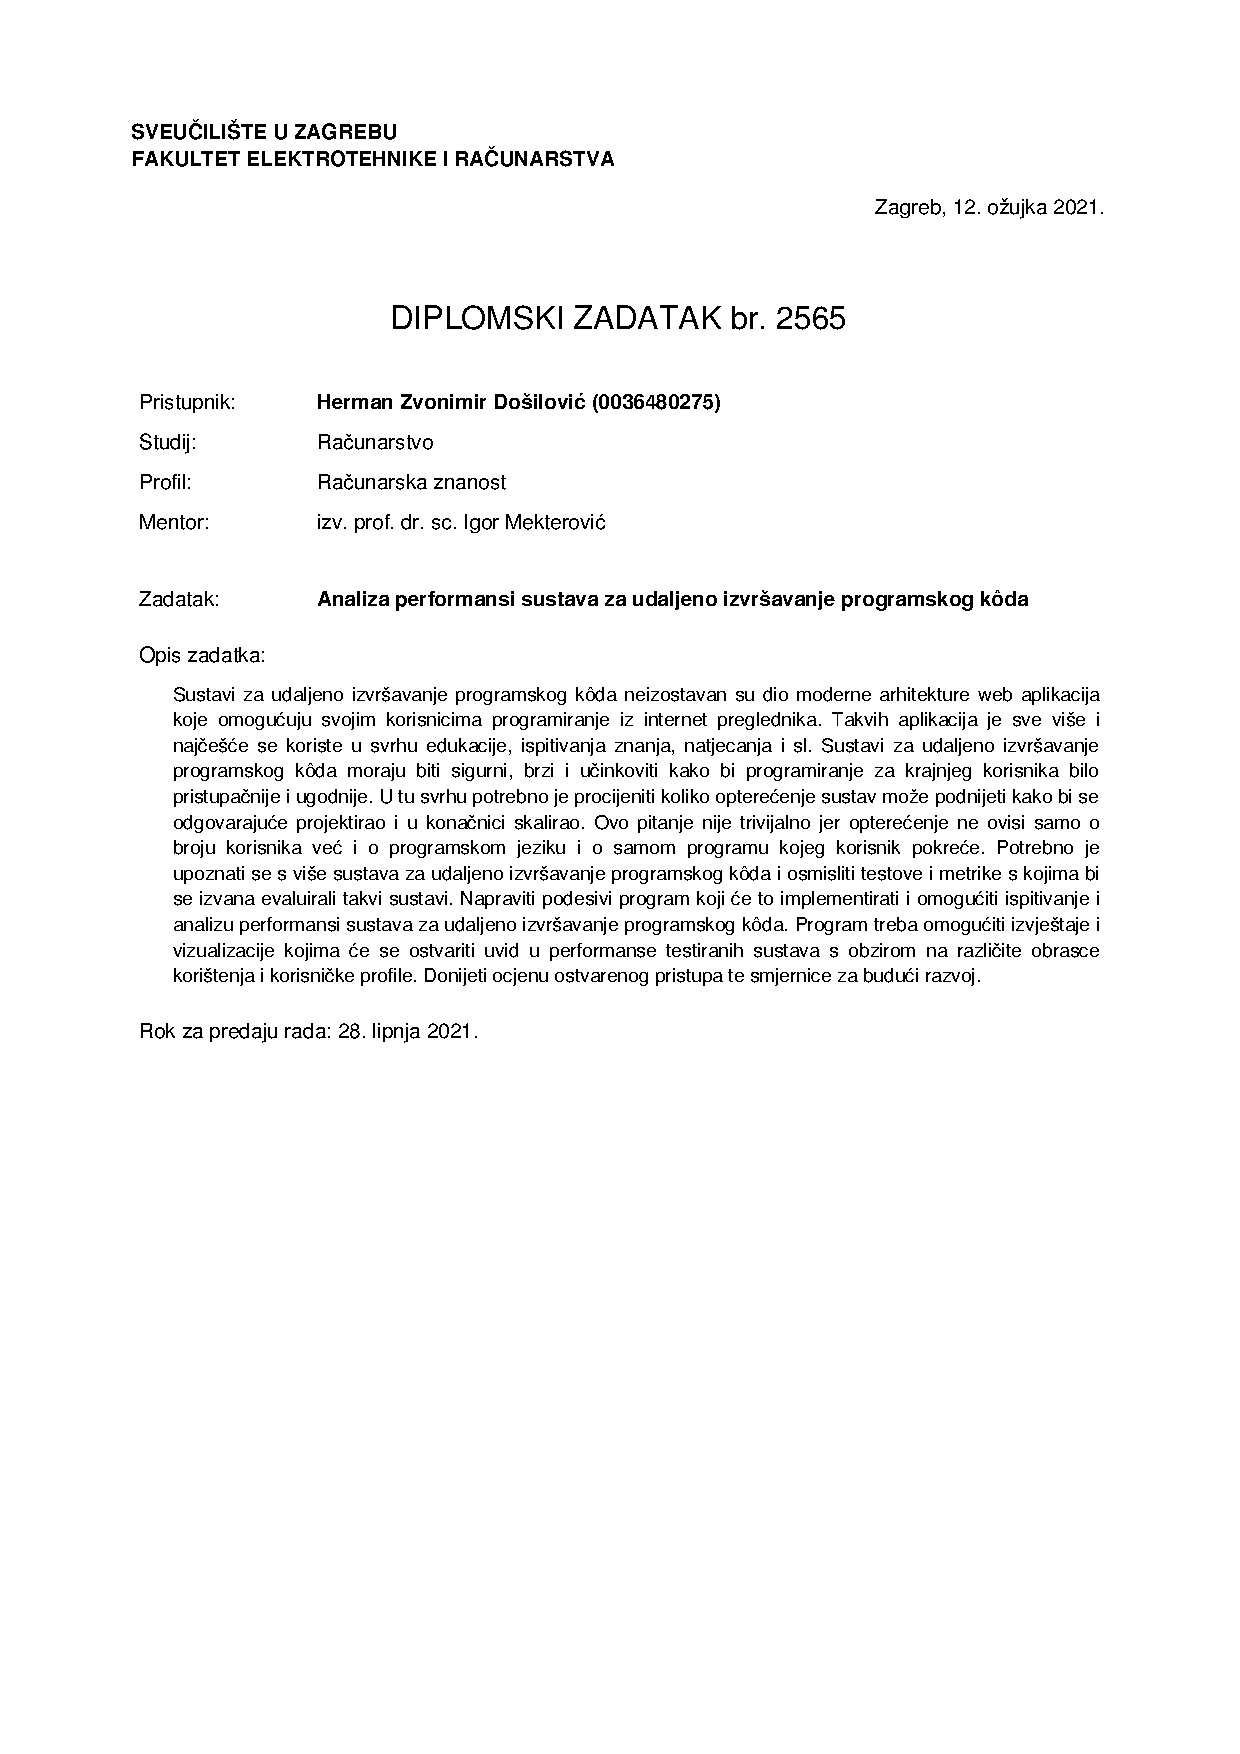
\includepdf[pages=-]{hr_0036480275_56.pdf}

\zahvala{Deo grátias.}

\tableofcontents

\chapter{Uvod}
Računarsko razmišljanje \engl{computational thinking} je termin kojeg je prvi put upotrijebio Seymour Aubrey Papert 1980.\ godine u svojoj knjizi \textit{Mindstorms: Children, Computers, and Powerful Ideas} \citep{10.5555/1095592} u kojoj, između ostalog, razmatra korištenje računala kao alata koji može utjecati na način na koji ljudi uče i razmišljaju. Njegova vizija korištenja računala u edukaciji djece bila je naučiti djecu programirati računalo s ciljem da djeca već u ranoj dobi dotaknu neke od najdubljih ideja iz raznih znanstvenih disciplina. Papert programiranje računala opisuje kao komunikaciju između čovjeka i računala jezikom koji oboje razumiju, i time je njegova ideja razvoja računala, s kojim je prirodno naučiti  komunicirati, temeljna ideja koja se provlači kroz cijelu knjigu. Njegove ideje i inovacije promijenile su način na koji milijuni djece stvaraju i uče \citep{Papert.MITMediaLab}.

Termin \textit{računarsko razmišljanje} ponovo dobiva značajnu pažnju akademske zajednice \citep{grover2013computational} 2006.\ godine objavom istoimenog rada Jeannette M.\ Wing  koja računarsko razmišljanje svrstava u fundamentalnu vještinu pored čitanja, pisanja i aritmetike \citep{wing2006computational}. Njezin je rad potaknuo intenzivnije istraživanje o važnosti uključivanja računarskog razmišljanja u edukacijski sustav \citep{lockwood2017computational}. U svom izvješću iz 2014.\ godine internacionalna neprofitna organizacija European Schoolnet prepoznala je važnost integracije računarskog razmišljanja u edukacijski sustav te navode da već tada programiranje počinje biti sve ključnija vještina koju će morati steći svi mladi, ali i radnici iz širokog spektra industrije \citep{balanskat2014computing}. Navode, također, da je programiranje dio logičkog rasuđivanja i da ono pripada ključnim vještinama 21.\ stoljeća, što dodatno potkrjepljuje ideje Jeannette M.\ Wing iz 2006.\ godine.

Programiranje je od 2015.\ godine uključeno u nastavni plan i program 16 Europskih zemalja koje kod svojih učenika žele razviti vještine logičkog razmišljanja i rješavanja problema, ali i povećati mogućnost zapošljavanja \citep{balanskat2015computing}. Budući da se vještina programiranja stječe vježbanjem \citep{kurnia2001online}, institucije, koje u svom nastavnom planu i programu nude programiranje, svojim studentima trebaju omogućiti pristup biblioteci problemskih zadataka. Programska rješenja studenata konačno netko treba i ocijeniti, a tradicionalno ručno ocjenjivanje programskog kôda unosi dodatne probleme \citep{kurnia2001online}.

Probleme koje unosi tradicionalno ručno ocjenjivanje programskog kôda rješavaju \textbf{sustavi za udaljeno ocjenjivanje} (engl.\ \textit{online judges}, krat.\ \textit{OJs}) koji poboljšavaju proces edukacije i ocjenjivanja, ali i omogućuju studentima da prevedu \engl{compile} i izvrše \engl{execute} svoj programski kôda prije predaje \citep{wang2021metaoj}. Sustavi za udaljeno ocjenjivanje, poput \textit{web} aplikacije Edgar \citep{mekterovic2020building} razvijene na Fakultetu elektrotehnike i računarstva Sveučilišta u Zagrebu, omogućuju nastavnicima izradu \textit{online} provjera znanja koje pomoću ispitnih primjera automatski ocjenjuju rješenja studenata predana u obliku programskog kôda i time ubrzavaju proces ispravljanja i ocjenjivanja, i smanjuju mogućnost uvođenja grešaka koje se mogu dogoditi prilikom ručnog ocjenjivanja. Također, sustavi za udaljeno ocjenjivanje omogućuju studentima brzi pristup problemskim zadacima koje mogu rješavati i time vježbati svoju vještinu programiranja. Sustavi za udaljeno ocjenjivanje najčešće omogućuju studentima programiranje u pregledniku odnosno kroz \textit{web} aplikaciju koju koristi njihova institucija. Mogućnost programiranja i predaje rješenja kroz \textit{web} aplikaciju olakšava studentima, pogotovo početnicima, proces postavljanja okoline za programiranje u programskom jeziku koji pokriva nastavni plan i program koji pohađaju.

Jasno je dakle da se programski kôd studenta ne može prevesti i izvršiti direktno na njegovom računalu budući da na njemu nema postavljenju okolinu koja to omogućuje. Programski kôd studenta kojeg piše u svom pregledniku izvršava se na poslužitelju sustava za udaljeno ocjenjivanje. Sustav za udaljeno ocjenjivanje, poput već spomenute \textit{web} aplikacije Edgar, oslanja se na \textbf{sustav za udaljeno izvršavanje programskog kôda} (engl.\ \textit{online code execution system}, krat.\ \textit{OCES}) koji mu osigurava da će se programski kôd studenta prevesti i izvršiti bez negativnih posljedica za poslužitelj i ostalih korisnika aplikacije. Stoga OCES predstavlja ključnu komponentu u arhitekturi sustava za udaljeno ocjenjivanje o kojoj ovisi prije svega sigurnost i integritet poslužitelja, a zatim i korisničko iskustvo, i kvaliteta usluge.

Sustavi za udaljeno izvršavanje programskog kôda nude \textit{web} aplikacijsko sučelje koje sustavi za udaljeno ocjenjivanje mogu transparentno koristiti za stvaranje zahtjeva za izvršavanje programskog kôda, dohvat informacija o izvršavanju i dohvat rezultata izvršavanja. Sučelje koje takvi sustavi nude je jednostavno za korištenje, međutim, usluga koju nude je resursno i sigurnosno zahtjevna. Dobro izveden i skaliran sustav za udaljeno izvršavanje programskog kôda donosi veliku vrijednost sustavima za udaljeno ocjenjivanje budući da se razvojni inženjeri tih sustava tada mogu u potpunosti fokusirati na razvoj proizvoda i njegovih funkcionalnosti što krajnjem korisniku donosi bolje korisničko iskustvo i kvalitetniju uslugu.

Budući da se sustavi za udaljeno izvršavanje programskog kôda u literaturi razmatraju kao zasebne komponente arhitekture sustava za udaljeno ocjenjivanje tek od \citep{9245310}, ne postoji u literaturi radni okvir za analizu performansi i ocjenu kvalitete i pouzdanosti takvih sustava. Performanse, kvaliteta i pouzdanost sustava za udaljeno izvršavanje programskog kôda dolaze do izražaja pri intenzivnom višekorisničkom opterećenju koje, u kontekstu sustava za udaljeno izvršavanje programskog kôda, predstavljaju zahtjevi za izvršavanje programskog kôda koje sustav dobiva kroz \textit{web} aplikacijsko sučelje.

Ovaj rad predstavlja prvi radni okvir za analizu performansi i ocjenu kvalitete i pouzdanosti usluge koju nude sustavi za udaljeno izvršavanje programskog kôda. Ovaj rad također predstavlja i aplikaciju Hélory\footnote{Sv.\ Ivo Hélory (1253.\ -- 1303.), po kome je aplikacija dobila ime, zaštitnik je, između ostalog i sudaca \engl{judges}.} koja implementira predstavljeni radni okvir za analizu performansi i ocjenu kvalitete i pouzdanosti za tri sustava za udaljeno izvršavanje programskog kôda: Sphere Engine, Piston i Judge0. Razvijen u obliku komandno-linijske aplikacije, Hélory nudi jednostavno pokretanje višekorisničkog opterećenja na željenom sustavu, a nakon eksperimenta Hélory će generirati i pohraniti izvještaj o pokrenutom eksperimentu koji sadrži detaljne informacije o svakom pojedinom zahtjevu za izvršavanje i grafički prikaz metrika od interesa.

U poglavlju \ref{chap:oj-ecosystem} opisana je arhitektura OJ ekosustava, dan je pregled slučajeva uporabe \engl{use-cases} i opisana je problematika udaljenog izvršavanja programskog kôda. Dodatno, poglavlje \ref{chap:oj-ecosystem} donosi formalnu definiciju OCES-a kroz funkcionalne i nefunkcionalne zahtjeve, i daje pregled sustava koje Hélory podržava. Poglavlje \ref{chap:analysis} predstavlja radni okvir za analizu performansi i ocjenu kvalitete i pouzdanosti usluge OCES-a, dok poglavlje \ref{chap:helory} daje pregled funkcionalnosti razvijene aplikacije Hélory. U poglavlju \ref{chap:use} pokazuje se primjer korištenja aplikacije Hélory u analizi performansi sustava Piston i Judge0. Konačno, poglavlje \ref{chap:future} daje smjernice za budući razvoj radnog okvira i aplikacije Hélory.

\chapter{Arhitektura ekosustava sustava za udaljeno ocjenjivanje}
\label{chap:oj-ecosystem}
Sustavi za udaljeno ocjenjivanje dio su arhitekture OJ ekosustava prikazane na slici \ref{fig:oj-ecosystem}, a koja započinje zaštićenim okruženjem \engl{sandbox} koje osigurava sigurno prevođenje i izvršavanje programskog kôda korisnika na poslužitelju, i završava specijaliziranim izvedbama sustava za udaljeno ocjenjivanje koji se koriste u raznim slučajevima uporabe. Ovo poglavlje daje pregled svake komponente arhitekture OJ ekosustava i motivaciju za njezino korištenje.

\begin{figure}[htb]
	\centering
	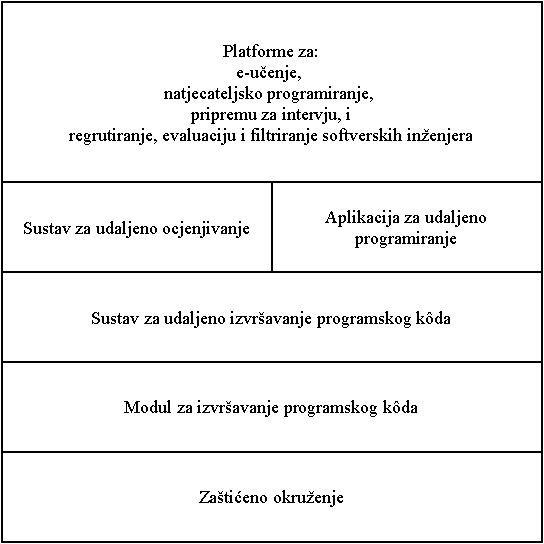
\includegraphics[width=0.75\textwidth]{images/Ekosustav.pdf}
	\caption{
		Arhitektura OJ ekosustava. \citep{9245310}
	}
	\label{fig:oj-ecosystem}
\end{figure}

\pagebreak

\section{Zaštićeno okruženje}
Sustavi za udaljeno ocjenjivanje koriste se za evaluaciju programskog kôda korisnika na unaprijed zadanom skupu primjera za ispitivanje, što povlači pitanje gdje će se programski kôd korisnika prevesti i izvršiti budući da se bez toga ne može ocijeniti njegovo rješenje. Najjednostavnije bi bilo da korisnik samostalno prevede i izvrši svoj program, i da zatim u sustav postavi rješenja koja je dobio. Ovakav pristup bio bi u redu za napredne korisnike koji znaju instalirati i koristiti odgovarajući prevoditelj za odabrani programski jezik, međutim, za početnike bi ovakav pristup rezultirao jako lošim korisničkim iskustvom. Ovo naime nije jedini argument zašto nije dobro da korisnik samostalno prevodi, izvršava i postavlja rješenja svojih programa. Ispitni primjeri trebaju ostati nepoznati korisniku kako ih ne bi zloupotrijebio, jer je za neke zadatke dovoljno imati standardni ulaz \engl{standard input} iz kojeg se lako dobije očekivani izlaz \engl{expected output}. Već se samo sa ovim snažno opravdanim zahtjevom može zaključiti da je programski kôd korisnika potrebno izvršiti na poslužitelju kojem korisnik nema pristup. Ovakav zahtjev otvara novi spektar problema koje je potrebno riješiti i koji su opisani u \citep{kurnia2001online}.

Pokretanje programskog kôda korisnika na udaljenom poslužitelju nameće izazov da se korisnikov program mora pokrenuti u zaštićenom okruženju kako ne bi negativno utjecao na rad poslužitelja i ostalih procesa. Postoje razne tehnike opisane u \citep{yi2014comparison} koje se koriste za izvršavanje programskog kôda u zaštićenom okruženju, i u kontekstu sustava za udaljeno ocjenjivanje od zaštićenog okruženja očekujemo sljedeće funkcionalnosti:
\begin{itemize}
    \item[$\bullet$] inicijalizaciju zaštićenog okruženja,
    \item[$\bullet$] mogućnost prenošenja programskog kôda korisnika u zaštićeno okruženje,
    \item[$\bullet$] prevođenje i izvršavanje programskog kôda u zaštićenom okruženju uz navođenje procesorskih i memorijskih ograničenja,
    \item[$\bullet$] prikupljanje standardnog izlaza \engl{standard output} programa i ostalih meta podatka o izvršavanju, i
    \item[$\bullet$] čišćenje \engl{cleanup} zaštićenog okruženja.
\end{itemize}

Sustavi Judge0 i Piston, o kojima će biti riječ nešto kasnije u ovom poglavlju, koriste Isolate \citep{marevs2012new} i Docker \citep{merkel2014docker} kao zaštićena okruženja za prevođenje i izvršavanje programskog kôda. Isolate i Docker oboje koriste kontrolne grupe \engl{control groups}, značajke sustava Linux koje omogućuju definiranje resursnih ograničenja pojedinog procesa. Odabir korištenja jednog, odnosno drugog zaštićenog okruženja ovisi, između ostalog, o preferencijama razvojnih inženjera.

Važnost korištenja zaštićenog okruženja koje osigurava da programski kôd korisnika ne šteti radu poslužitelja i ostalih procesa prikazuju isječci \ref{lst:infinite-compilation} i \ref{lst:fork-bomb} napisani u programskom jeziku C. 

Isječak \ref{lst:infinite-compilation} prikazuje ispravan C program koji uključuje uređaj pseudo-slučajnih brojeva sustava Linux. Budući da uređaj generira beskonačni slijed pseudo-slučajnih brojeva, uključivanje tog uređaja dovodi do beskonačnog vremena prevođenja. Ukoliko više korisnika napravi zahtjev za izvršavanjem ovakvog ili sličnog programa, na poslužitelju brzo dolazi do iscrpljivanja procesorskih i memorijskih resursa i time postaje neupotrebljiv. Iz ovog je jednostavnog primjera jasno da je proces prevođenja potrebno pokrenuti u zaštićenom okruženju koje će imati ograničene procesorske i memorijske resurse.

\

\begin{lstlisting}[
    caption={Ispravan C program s beskonačnim vremenom prevođenja.},
    label={lst:infinite-compilation},
    language=c
]
#include </dev/random>
int main() {
    return 0;
}
\end{lstlisting}

Izoliranje izvršavanja programskog kôda korisnika još je važnije od izolacije prevođenja, budući da je za zloupotrebu neizoliranog procesa prevođenja potrebno nešto više znanja o prevodiocima i programskom jeziku koji se koristi. Isječak \ref{lst:fork-bomb} prikazuje C program koji će beskonačno mnogo puta stvoriti novi proces, i svaki novostvoreni proces napravit će isto. Broj novostvorenih procesa može se opisati eksponencijalnom funkcijom $f(x) = 2^x$, gdje je $x$ broj ponavljanja petlje. Dovoljno je da jedan korisnik pokrene ovakav program da se na poslužitelju iscrpe procesorski i memorijski resursi koji će ga učiniti neupotrebljivim.

\

\begin{lstlisting}[
    caption={C program s beskonačnim grananjem novih procesa.},
    label={lst:fork-bomb},
    language=c
]
#include <unistd.h>
int main() {
    while(1) {
        fork();
    }
    return 0;
}
\end{lstlisting}

Oba isječka potvrđuju da je u sustavima za udaljeno ocjenjivanje nužno koristiti zaštićeno okruženje koja će prevesti i izvršiti programski kôd svakog korisnika. 

Gledajući iz perspektive sustava za udaljeno ocjenjivanje svaki programski kôd korisnika smatra se opasnim za poslužitelj, stoga se u kontekstu sustava za udaljeno ocjenjivanje govori o nepouzdanom programskom kôdu \engl{untrusted source code} kojeg je potrebno prevesti i izvršiti.

\section{Modul za izvršavanje programskog kôda}
Modul za izvršavanje programskog kôda (engl.\ \textit{code execution engine}, krat.\ \textit{CEE}) iduća je komponenta u arhitekturi OJ ekosustava koja koristi zaštićeno okruženje za prevođenje i izvršavanje programskog kôda, i koja zatim obrađuje meta podatke o prevođenju i izvršavanju koje generira zaštićeno okruženje. Slika \ref{fig:cee-and-sandbox} prikazuje dijagram toka interakcije između modula za izvršavanje programskog kôda i zaštićenog okruženja.

\begin{figure}[htb]
	\centering
	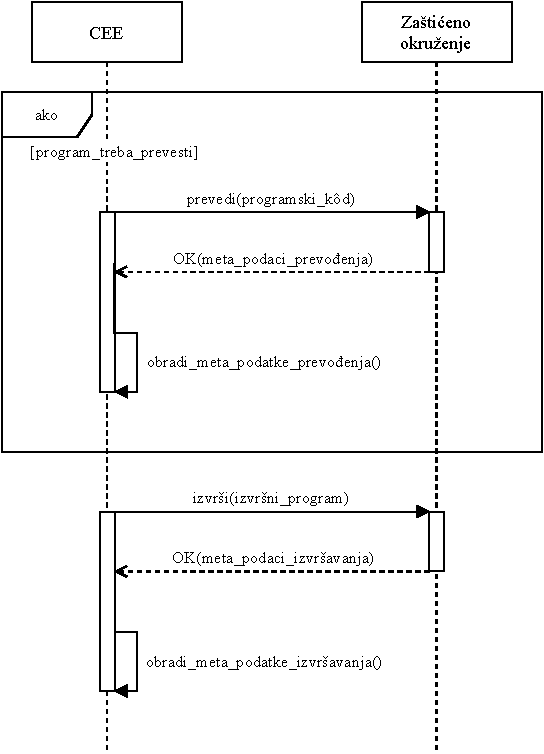
\includegraphics[width=0.61\textwidth]{images/CEE i zasticeno okruzenje.pdf}
	\caption{
		Interakcija modula za izvršavanje programskog kôda s zaštićenim okruženjem.
	}
	\label{fig:cee-and-sandbox}
\end{figure}

\pagebreak

\section{Sustav za udaljeno izvršavanje programskog kôda}
Sustav za udaljeno izvršavanje programskog kôda je sustav koji nudi \textit{web} aplikacijsko sučelje \engl{web API} za prevođenje i izvršavanje proizvoljnog programskog kôda. Arhitekturalni prikaz na slici \ref{fig:oj-ecosystem} izdvaja sustav za udaljeno izvršavanje programskog kôda kao zasebnu komponentu na koju se oslanjaju sustav za udaljeno ocjenjivanje, aplikacija za udaljeno programiranje, a zatim i specijalizirane izvedbe sustava za udaljeno ocjenjivanje razvijene za specifičan slučaj uporabe. Sustav za udaljeno izvršavanje programskog kôda najčešće je strogo povezan i zavisan o ostatku komponenata u arhitekturu sustava za udaljeno ocjenjivanje \citep{9245310}, međutim, u ovom radu razmatraju se oni sustavi za udaljeno izvršavanje programskog kôda koji su neovisni o ostatku arhitekture koja se na njih oslanja.

Slika \ref{fig:oces-architecture} prikazuje dijagram komponenti sustava za udaljeno izvršavanje programskog kôda koji preko \textit{web} aplikacijskog sučelja nudi uslugu izvršavanja programskog kôda (lijeva priključnica na slici \ref{fig:oces-architecture}) koju koriste sustav za udaljeno ocjenjivanje ili aplikacije za udaljeno programiranje. 

\begin{figure}[htb]
	\centering
	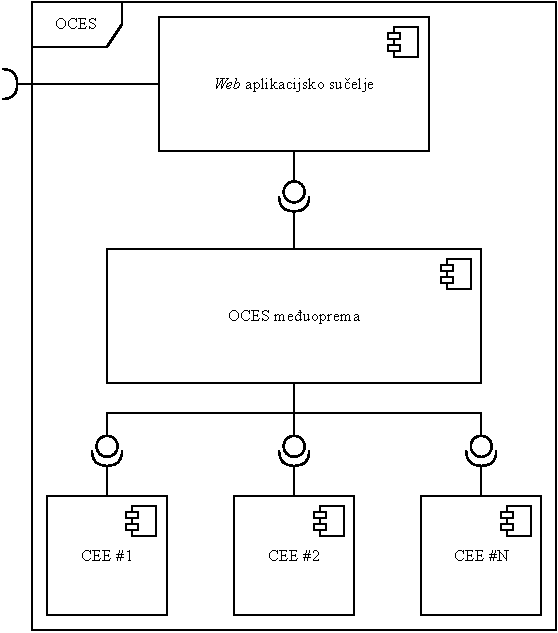
\includegraphics[width=0.6\textwidth]{images/Arhitektura OCES-a.pdf}
	\caption{
		Dijagram komponenti sustava za udaljeno izvršavanje programskog kôda.
	}
	\label{fig:oces-architecture}
\end{figure}

\pagebreak

Putem OCES međuopreme \engl{middleware}, zahtjev za izvršavanje programskog kôda dolazi do modula za izvršavanje programskog kôda kojih u sustavu može biti više kako bi se prilikom intenzivnog višekorisničkog opterećenja zahtjevi za izvršavanje efikasnije obavili. Način izvedbe OCES međuopreme ovisi o pojedinom sustavu za udaljeno izvršavanje programskog kôda kao što se npr.\ međuoprema sustava Judge0 sastoji od PostgreSQL baze podataka koja pohranjuje sve zahtjeve za izvršavanje programskog kôda i rezultate prevođenja i izvršavanja, i Redis baze podataka koja se koristi kao red poslova \engl{job queue} \citep{9245310}.

Formalna definicija sustava za udaljeno izvršavanje programskog kôda dana je u \citep{9245310} kroz funkcionalne i nefunkcionalne zahtjeve. Funkcionalni zahtjevi podijeljeni su u nužne i dovoljne, odnosno na zahtjeve koje sustav nužno mora ispuniti i dodatne neobavezne zahtjeve. Nefunkcionalni zahtjevi su također neobavezni, ali preporučeni.

\subsubsection{Funkcionalni zahtjevi}
Sustav za udaljeno izvršavanje programskog kôda \textbf{mora} pružiti:
\begin{itemize}
    \item[$\bullet$] dobro dokumentirano \textit{web} aplikacijsko sučelje,
    \item[$\bullet$] podršku za prevođenje i izvršavanje proizvoljnog programskog kôda za barem jedan programski jezik,
    \item[$\bullet$] izvršavanje u zaštićenom okruženju s pretpostavljenim procesorskim i memorijskim ograničenjima,
    \item[$\bullet$] podršku za navođenje proizvoljnog standardnog ulaza, i
    \item[$\bullet$] podršku za dohvat rezultata izvršavanja programa koji sadrži barem standardni izlaz programa.
\end{itemize}

Dodatno, ali neobavezno, sustav za udaljeno izvršavanje programskog kôda \textbf{može} pružiti podršku za:
\begin{itemize}
    \item[$\bullet$] navođenje dodatnih opcija prevodioca,
    \item[$\bullet$] navođenje komandno-linijskih argumenata,
    \item[$\bullet$] navođenje resursnih ograničenja poput npr.\ procesorskih i memorijskih ograničenja,
    \item[$\bullet$] inicijalizaciju zaštićenog okruženja s dodatnim datotekama,
    \item[$\bullet$] dohvat detaljnih meta podataka o izvršavanju programa (npr.\ vrijeme izvođenja programa ili sadržaj standardnog izlaza za pogreške \engl{standard error}),
    \item[$\bullet$] skupne zahtjeve za izvršavanje,
    \item[$\bullet$] višestruke standardne ulaze, i
    \item[$\bullet$] autentifikaciju.
\end{itemize}

Čim više funkcionalnih zahtjeva sustav ispunjava tim više slučajeva uporabe može zadovoljiti. \citep{9245310}

\subsubsection{Nefunkcionalni zahtjevi}
Preporuča se da sustav za udaljeno izvršavanje programskog kôda bude:
\begin{itemize}
    \item[$\bullet$] skalabilan,
    \item[$\bullet$] konfigurabilan,
    \item[$\bullet$] siguran,
    \item[$\bullet$] lako upogonljiv,
    \item[$\bullet$] efikasan,
    \item[$\bullet$] otporan,
    \item[$\bullet$] proširiv, i
    \item[$\bullet$] robustan.
\end{itemize}

Čim više nefunkcionalnih zahtjeva sustav ispunjava tim ga je lakše integrirati u sustav specifično izveden za pojedini slučaj uporabe \citep{9245310}. Skalabilnost i efikasnost sustava za udaljeno izvršavanje programskog kôda dolazi do izražaja prilikom izrazitog višekorisničkog opterećenja kada krajnji korisnici neposredno preko sustava za udaljeno ocjenjivanje stvaraju zahtjeve za izvršavanje. Tada se od sustava za udaljeno izvršavanje programskog kôda očekuje da neovisno o broju zahtjeva efikasno izvrši programski kôd korisnika i vrati rezultate izvršavanja sustavu za udaljeno ocjenjivanje jer će u protivnom krajnje korisničko iskustvo biti narušeno dugim vremenom čekanja. Konfigurabilnost i proširivost sustava za udaljeno izvršavanje programskog kôda omogućuje razvojnim inženjerima da sustav prilagode svojim zahtjevima prilikom razvoja sustava za određeni slučaj uporabe. Laka upogonljivost sustava za udaljeno izvršavanje programskog kôda omogućava razvojnim inženjerima da brzo napreduju u razvoju sustava za određeni slučaj uporabe. Sigurnost sustava za udaljeno izvršavanje programskog kôda uvelike ovisi načinu na koji sustav iskorištava funkcionalnosti zaštićene okoline i koristi li ju uopće. Od sustava se očekuje da niti jedan programski kôd ne naruši sigurnost i integritet poslužitelja. Ako se i dogodi da neki programski kôd uzrukuje neuobičajeno ponašanje, od sustava se očekuje da bude otporan i robustan na unutarnje pogreške koje se mogu dogoditi i da neovisno o njima vrati korisniku rezultat izvođenja.

U nastavku ove cjeline dan je pregled tri različita sustava za udaljeno izvršavanje programskog kôda koje podržava aplikacija Hélory.

\subsection{Sustav Sphere Engine}
Sustav za udaljeno izvršavanje programskog kôda Sphere Engine razvila je Poljska tvrtka Sphere Research Labs 2008.\ godine. Sphere Engine je jedan od vodećih komercijalnih sustava za udaljeno izvršavanje programskog kôda kojeg koristi više od 1000 institucija u 180 država. Jedna od najpoznatijih \textit{web} aplikacija koja koristi Sphere Engine je SPOJ \citep{SPOJ} koju je razvila ista tvrtka, a na kojoj korisnici mogu rješavati razne problemske zadatke iz domene natjecateljskog programiranja. Osim SPOJ-a, CodeChef \citep{CodeChef} također koristi Sphere Engine za udaljeno izvršavanje programskog kôda.

Budući da je Sphere Engine zatvoreni komercijalni sustav, nisu dostupne informacije o njegovoj izvedbi, niti o tome u kojim tehnologijama je razvijen.

U svrhu ovog rada dovoljno je spomenuti da sustav omogućuje prevođenje i izvršavanje programskog kôda u mnoštvo programskih jezika i da nudi bogatu dokumentaciju \textit{web} aplikacijskog sučelja.

\begin{figure}[htb]
	\centering
	
\includegraphics[width=\textwidth]{images/Sphere Engine Logo.png}
	\caption{
	    Vizualni identitet sustava Sphere Engine. \citep{SphereEngine}
	}
\end{figure}

\pagebreak

\subsection{Sustav Piston}
Sustav za udaljeno izvršavanje programskog kôda Piston \citep{Piston} je sustav otvorenog kôda koji je dostupan na platformi GitHub. Razvijen je i koristi se u edukativne svrhe zajednice koju vodi autor projekta.

Kao zaštićeno okruženje u kojoj se izvršava programski kôda korisnika, sustav Piston koristi Docker i nudi oskudnu dokumentaciju \textit{web} aplikacijskog sučelja, međutim, kao i Sphere Engine, podržava mnoštvo programskih jezika koji se mogu koristiti. Zajednica koja razvija sustav Piston također je razvila i komandno-linijsku aplikaciju koja se povezuje sa sustavom i tako korisnicima omogućava da iz ljuske \engl{shell} pokrenu proizvoljni programski kôd, dobivajući tako privid da se njihov program izvršio izravno na njihovom računalu.

\begin{figure}[htb]
	\centering
	
\includegraphics[width=0.45\textwidth]{images/Piston Logo.png}
	\caption{
	    Vizualni identitet sustava Piston. \citep{Piston}
	}
\end{figure}

\pagebreak

\subsection{Sustav Judge0}
Razvoj sustava Judge0 započet je 22.\ kolovoza 2016.\ godine na inicijativu autora ovog rada. Cilj razvoja sustava Judge0 bio je izgradnja novog, robustnog, skalabilnog i lako uporabljivog sustava za udaljeno izvršavanje programskog kôda koji se može jednostavno integrirati u razne \textit{web} aplikacije koje trebaju funkcionalnost izvršavanja programskog kôda. Razvijen je u programskom jeziku Ruby koristeći radni okvir Ruby on Rails, a kao zaštićeno okruženje koristi Isolate \citep{marevs2012new} koji se također koristi u popularnom sustavu za udaljeno ocjenjivanje CMS \citep{maggiolo2012introducing}. Sustav CMS koristio se na najvećim međunarodnim natjecanjima iz natjecateljskog programiranja poput informatičke olimpijade (IOI) i srednjoeuropske informatičke olimpijade (CEOI) \citep{CMSWeb}. Akademskoj zajednici sustav Judge0 napokon je formalno predstavljen 2020.\ godine radom \citep{9245310}.

\begin{figure}[htb]
	\centering
	
\includegraphics[width=0.65\textwidth]{images/Judge0 Logo.png}
	\caption[]{
	    Vizualni identitet sustava Judge0.\footnotemark
	}
\end{figure}

\footnotetext{Vizualni identitet sustava Judge0 osmislio je i izradio Emanuel Loborec.}

U vrijeme pisanja ovog rada, javna instanca sustava Judge0 izvršila je preko 12,7 milijuna programa korisnika diljem svijeta koji su sustav Judge0 integrirali u svoje proizvode. Dodatno, u vrijeme pisanja ovog rada, zabilježeno je preko 200 aktivnih instanci sustava Judge0 kojeg su razne organizacije pokrenule na svojim poslužiteljima. 

Od akademske godine 2018./2019. sustav Judge0 aktivno se koristi na Fakultetu elektrotehnike i računarstva Sveučilišta u Zagrebu kao integracijski dio \textit{web} aplikacije Edgar \citep{mekterovic2020building}. Time je sustav Judge0, neposredno preko \textit{web} aplikacije Edgar, koristilo preko 3000 studenata kroz nekoliko predmeta.

Sustav Judge0 odlikuje se prije svega bogatom dokumentacijom \textit{web} aplikacijskog sučelja koje omogućuje jednostavno korištenje sustava s mnoštvo konfiguracijskih opcija. Obilje funkcionalnosti koje nudi Judge0 omogućuje razvojnim inženjerima laku integraciju s drugim sustavima raznih slučajeva uporabe.

\begin{figure}[htb]
	\centering
	
\includegraphics[width=\textwidth]{images/Judge0 Clients.png}
	\caption{
	    Vizualni identiteti organizacija koje koriste sustav Judge0. \citep{Judge0Web}
	}
	\label{fig:judge0-clients}
\end{figure}

\pagebreak

\section{Sustav za udaljeno ocjenjivanje}
Sustav za udaljeno ocjenjivanje formalno je definiran u \citep{wasik2018survey} kao udaljena usluga \engl{online service} koja u oblaku \engl{cloud} izvodi barem jednu od sljedećih faza:
\begin{itemize}
    \item[$\bullet$] podnošenje zahtjeva za izvršavanje programskog kôda \engl{submission},
    \item[$\bullet$] procjena podnesenoga programskog kôda \engl{assessment}, i
    \item[$\bullet$] ocjenjivanje podnesenoga programskog kôda \engl{scoring}.
\end{itemize}

Podnošenje zahtjeva za izvršavanje programskog kôda podrazumijeva prihvaćanje programskog kôda u sustav, prevođenje po potrebi i verifikaciju da je program spreman za izvršavanje. U procjeni podnesenoga programskog kôda program se pokreće za svaki ispitni primjer i provjerava se uspješnost izvođenja programa sa zadanim procesorskim i memorijskim ograničenjima. Također, u istoj fazi, provjerava se standardni izlaz programa i uspoređuje ga se s očekivanim izlazom za trenutni ispitni primjer. Konačno, u fazi ocjenjivanja, dodjeljuje se ocjena na temelju rezultata iz prethodnih faza. Tako npr.\ na ocjenu u natjecateljskom programiranju može utjecati vrijeme koje je bilo potrebno natjecatelju da riješi pojedini zadatak. Što kasnije natjecatelj riješi ispravno zadatak to će manje bodova dobiti čak ako su mu svi ispitni primjeri ispravni uz zadana procesorska i memorijska ograničenja.

\pagebreak

\subsection{Interakcija sa sustavom za udaljeno izvršavanje programskog kôda}
\label{subsec:interaction}
Interakcija sustava za udaljeno ocjenjivanje i sustava za udaljeno izvršavanje programskog kôda može se dogoditi na dva načina: sinkrono i asinkrono.

Slika \ref{fig:sync-interaction} prikazuje dijagram toka sinkrone interakcije koja započinje zahtjevom za izvršavanjem koji OCES prihvati i u odgovoru vraća rezultate izvršavanja. Budući da izvršavanje programskog kôda može trajati i po nekoliko sekundi ova interakcija s OCES-om može iscrpiti njegove poslužiteljske resurse prilikom intenzivnog višekorisničkog opterećenja.

\

\begin{figure}[htb]
	\centering
	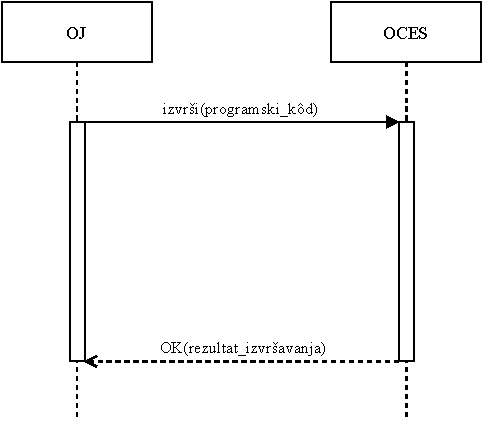
\includegraphics[width=0.8\textwidth]{images/Sync Interakcija.pdf}
	\caption{
		Sinkrona interakcija OJ-a i OCES-a.
	}
	\label{fig:sync-interaction}
\end{figure}

Asinkrona interakcija (slika \ref{fig:async-interaction}) započinje na isti način kao i sinkrona - zahtjevom za izvršavanje koji OCES prihvati, međutim, sada OCES vraća jedinstveni identifikator zahtjeva. Nakon što OJ primi jedinstveni identifikator svog zahtjeva na njemu je odgovornost da posebnim zahtjevom provjerava njegov status dok ne utvrdi da je izvršavanje završilo.

Sustav Piston podržava sinkronu interakciju, sustav Sphere Engine podržava asinkronu, dok sustav Judge0 podržava oba načina interakcije. Postoji zapravo još jedan način interakcije između OJ-a i OCES-a, a to je preko povratnog URL poziva \engl{URL callback}, međutim, u ovom radu takva vrsta interakcije se ne razmatra. Ukratko, prilikom stvaranja zahtjeva OJ navodi URL kojeg OCES mora iskoristiti za stvaranje povratnog zahtjeva koji u svom tijelu \engl{body} sadrži rezultat izvršavanja programa. Ovakva vrsta interakcije se ne razmatra u ovom radu jer klijent treba biti realiziran i kao poslužitelj koji može prihvatiti i obraditi povratni zahtjev koji dolazi od OCES-a. Sphere Engine i Judge0 podržavaju i ovakav način interakcije.

\

\begin{figure}[htb]
	\centering
	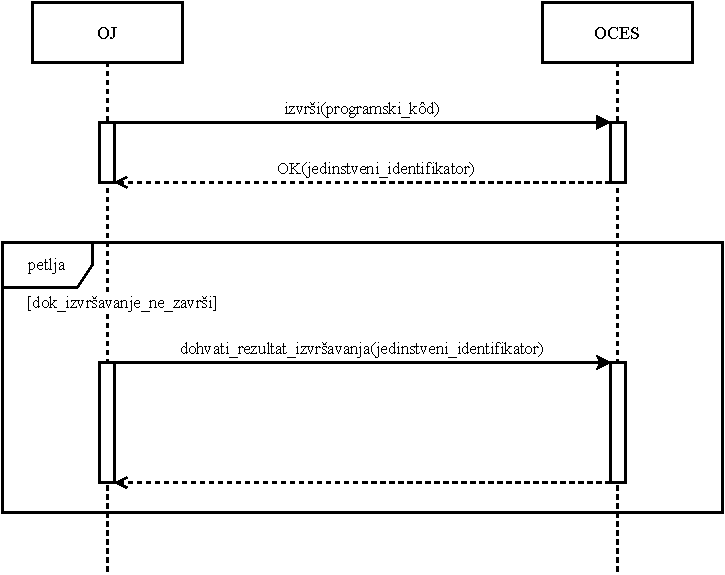
\includegraphics[width=\textwidth]{images/Async Interakcija.pdf}
	\caption{
		Asinkrona interakcija OJ-a i OCES-a.
	}
	\label{fig:async-interaction}
\end{figure}

\pagebreak

\section{\textit{Web} aplikacija za udaljeno programiranje}
\textit{Web} aplikacija za udaljeno programiranje poput aplikacije Judge0 IDE \citep{Judge0IDE} najjednostavniji je primjer uporabe sustava za udaljeno izvršavanje programskog kôda koje korisnicima omogućuju pisanje, prevođenje i izvršavanje programskog kôda u jednom od podržanih programskih jezika (slika \ref{fig:judge0-ide-ui}).

\begin{figure}[htb]
	\centering
	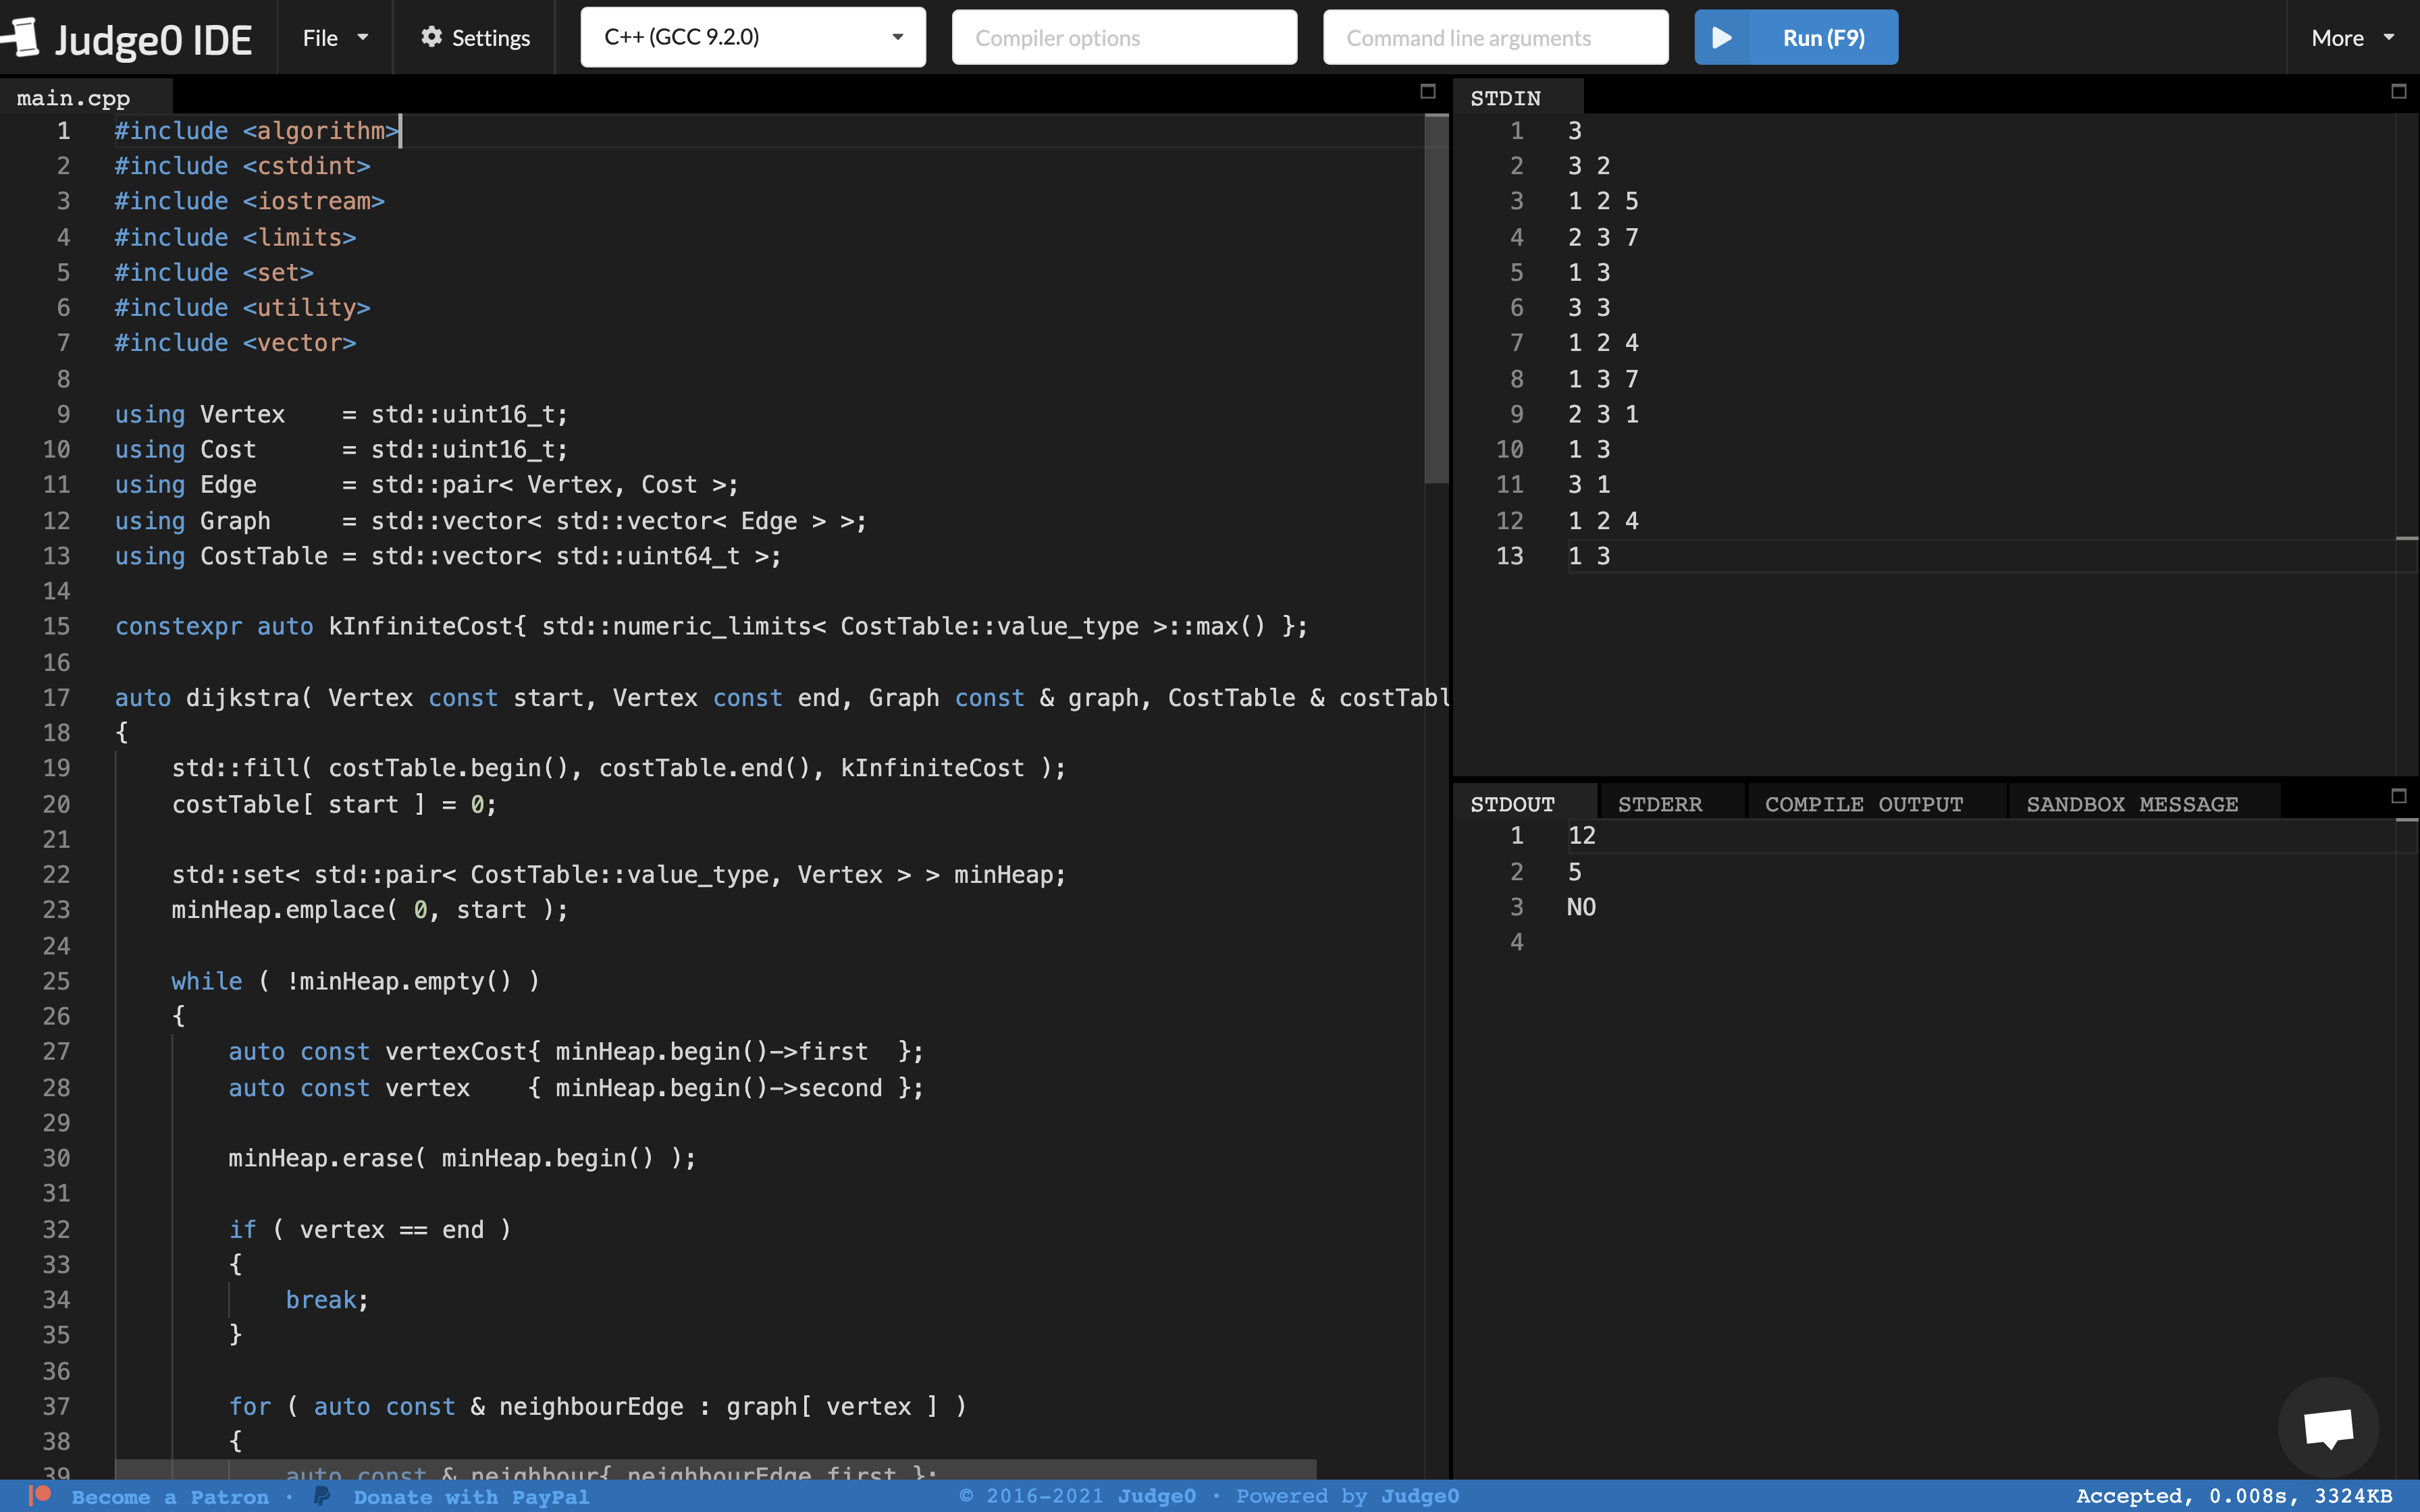
\includegraphics[width=\textwidth]{images/Judge0 IDE UI.png}
	\caption{
		Sučelje \textit{web} aplikacije Judge0 IDE.
	}
	\label{fig:judge0-ide-ui}
\end{figure}

\section{Specijalizirane izvedbe sustava za udaljeno ocjenjivanje}
Najčešća izvedba sustava za udaljeno ocjenjivanje su \textit{web} aplikacije za natjecateljsko programiranje poput: Codeforces \citep{Codeforces}, CodeChef \citep{CodeChef} i SPOJ \citep{SPOJ} gdje se od korisnika očekuje da iz teksta zadatka prepozna i implementira algoritam i odgovarajuću strukturu podataka koji će zadovoljiti zadana vremenska i memorijska ograničenja. 

Izvedba sustava za udaljeno ocjenjivanje kao \textit{web} aplikacije za e-učenje poput \textit{web} aplikacija Edgar \citep{mekterovic2020building} i CodeChum \citep{maranga2019codechum} koristi se za ocjenjivanje \engl{scoring} programskog kôda kojeg student prilaže kao rješenje zadatka iz npr.\ domaće zadaće ili provjere znanja.

\begin{figure}[htb]
	\centering
	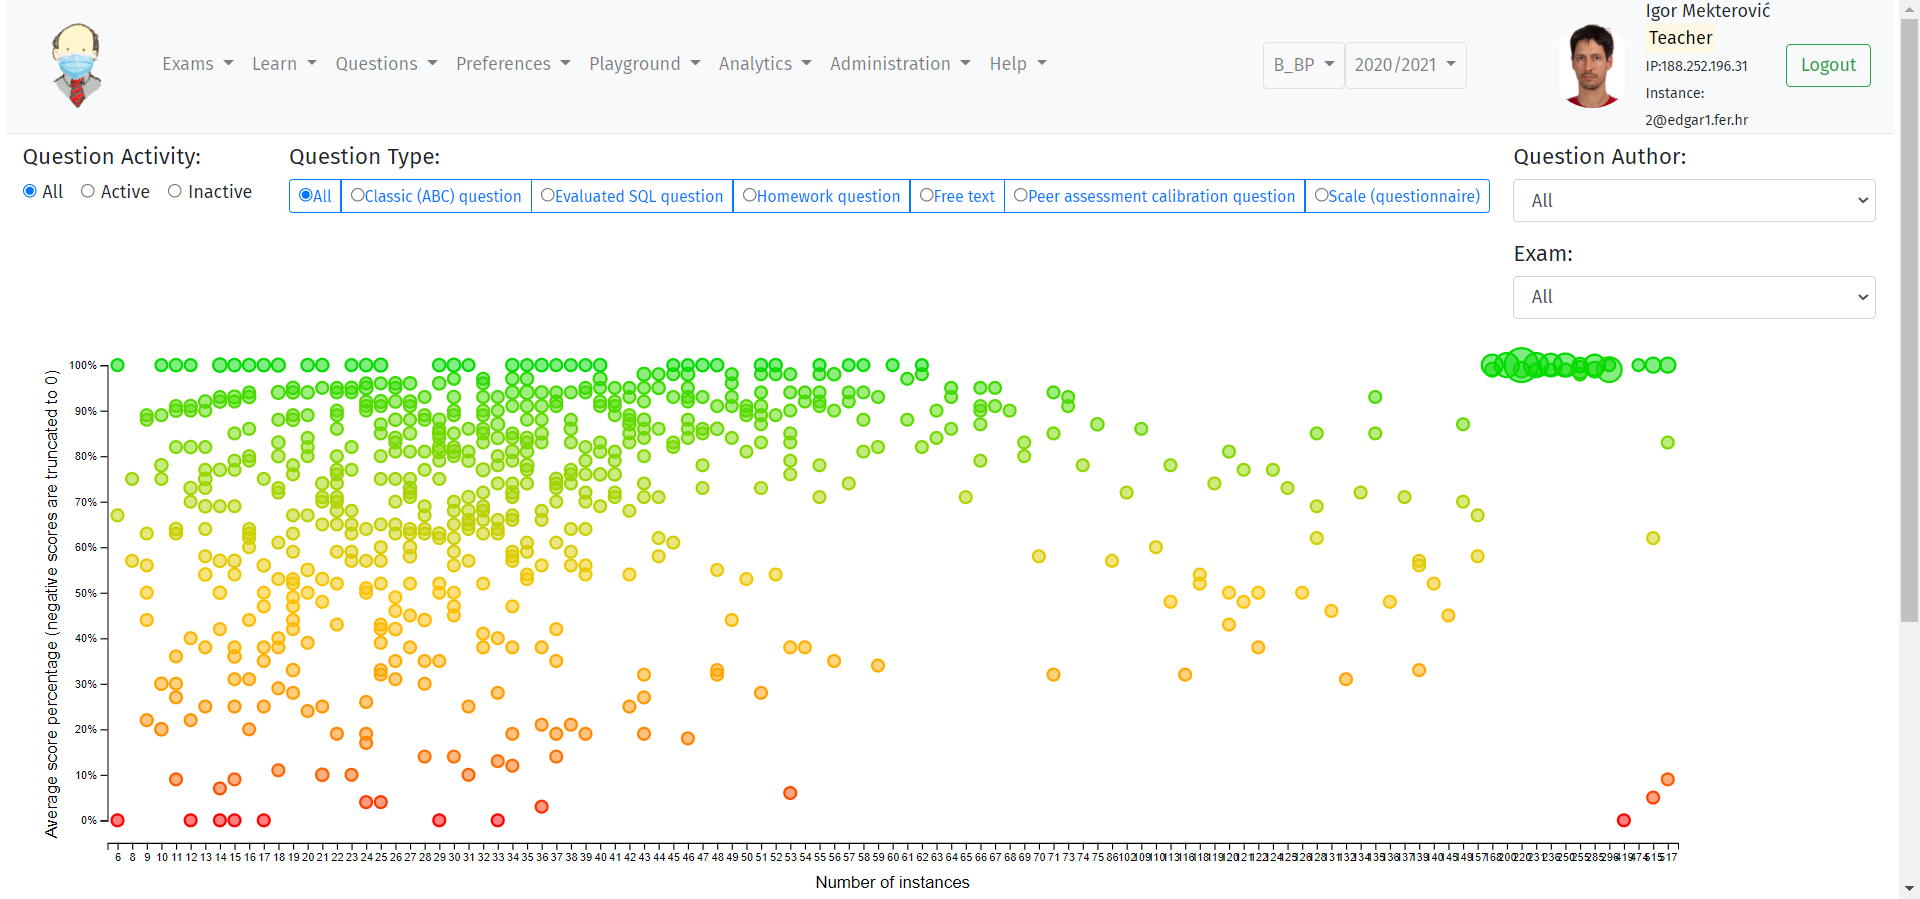
\includegraphics[width=\textwidth]{images/Edgar UI.png}
	\caption{
		Sučelje \textit{web} aplikacije Edgar iz perspektive učitelja.
	}
	\label{fig:edgar-ui}
\end{figure}

\begin{figure}[htb]
	\centering
	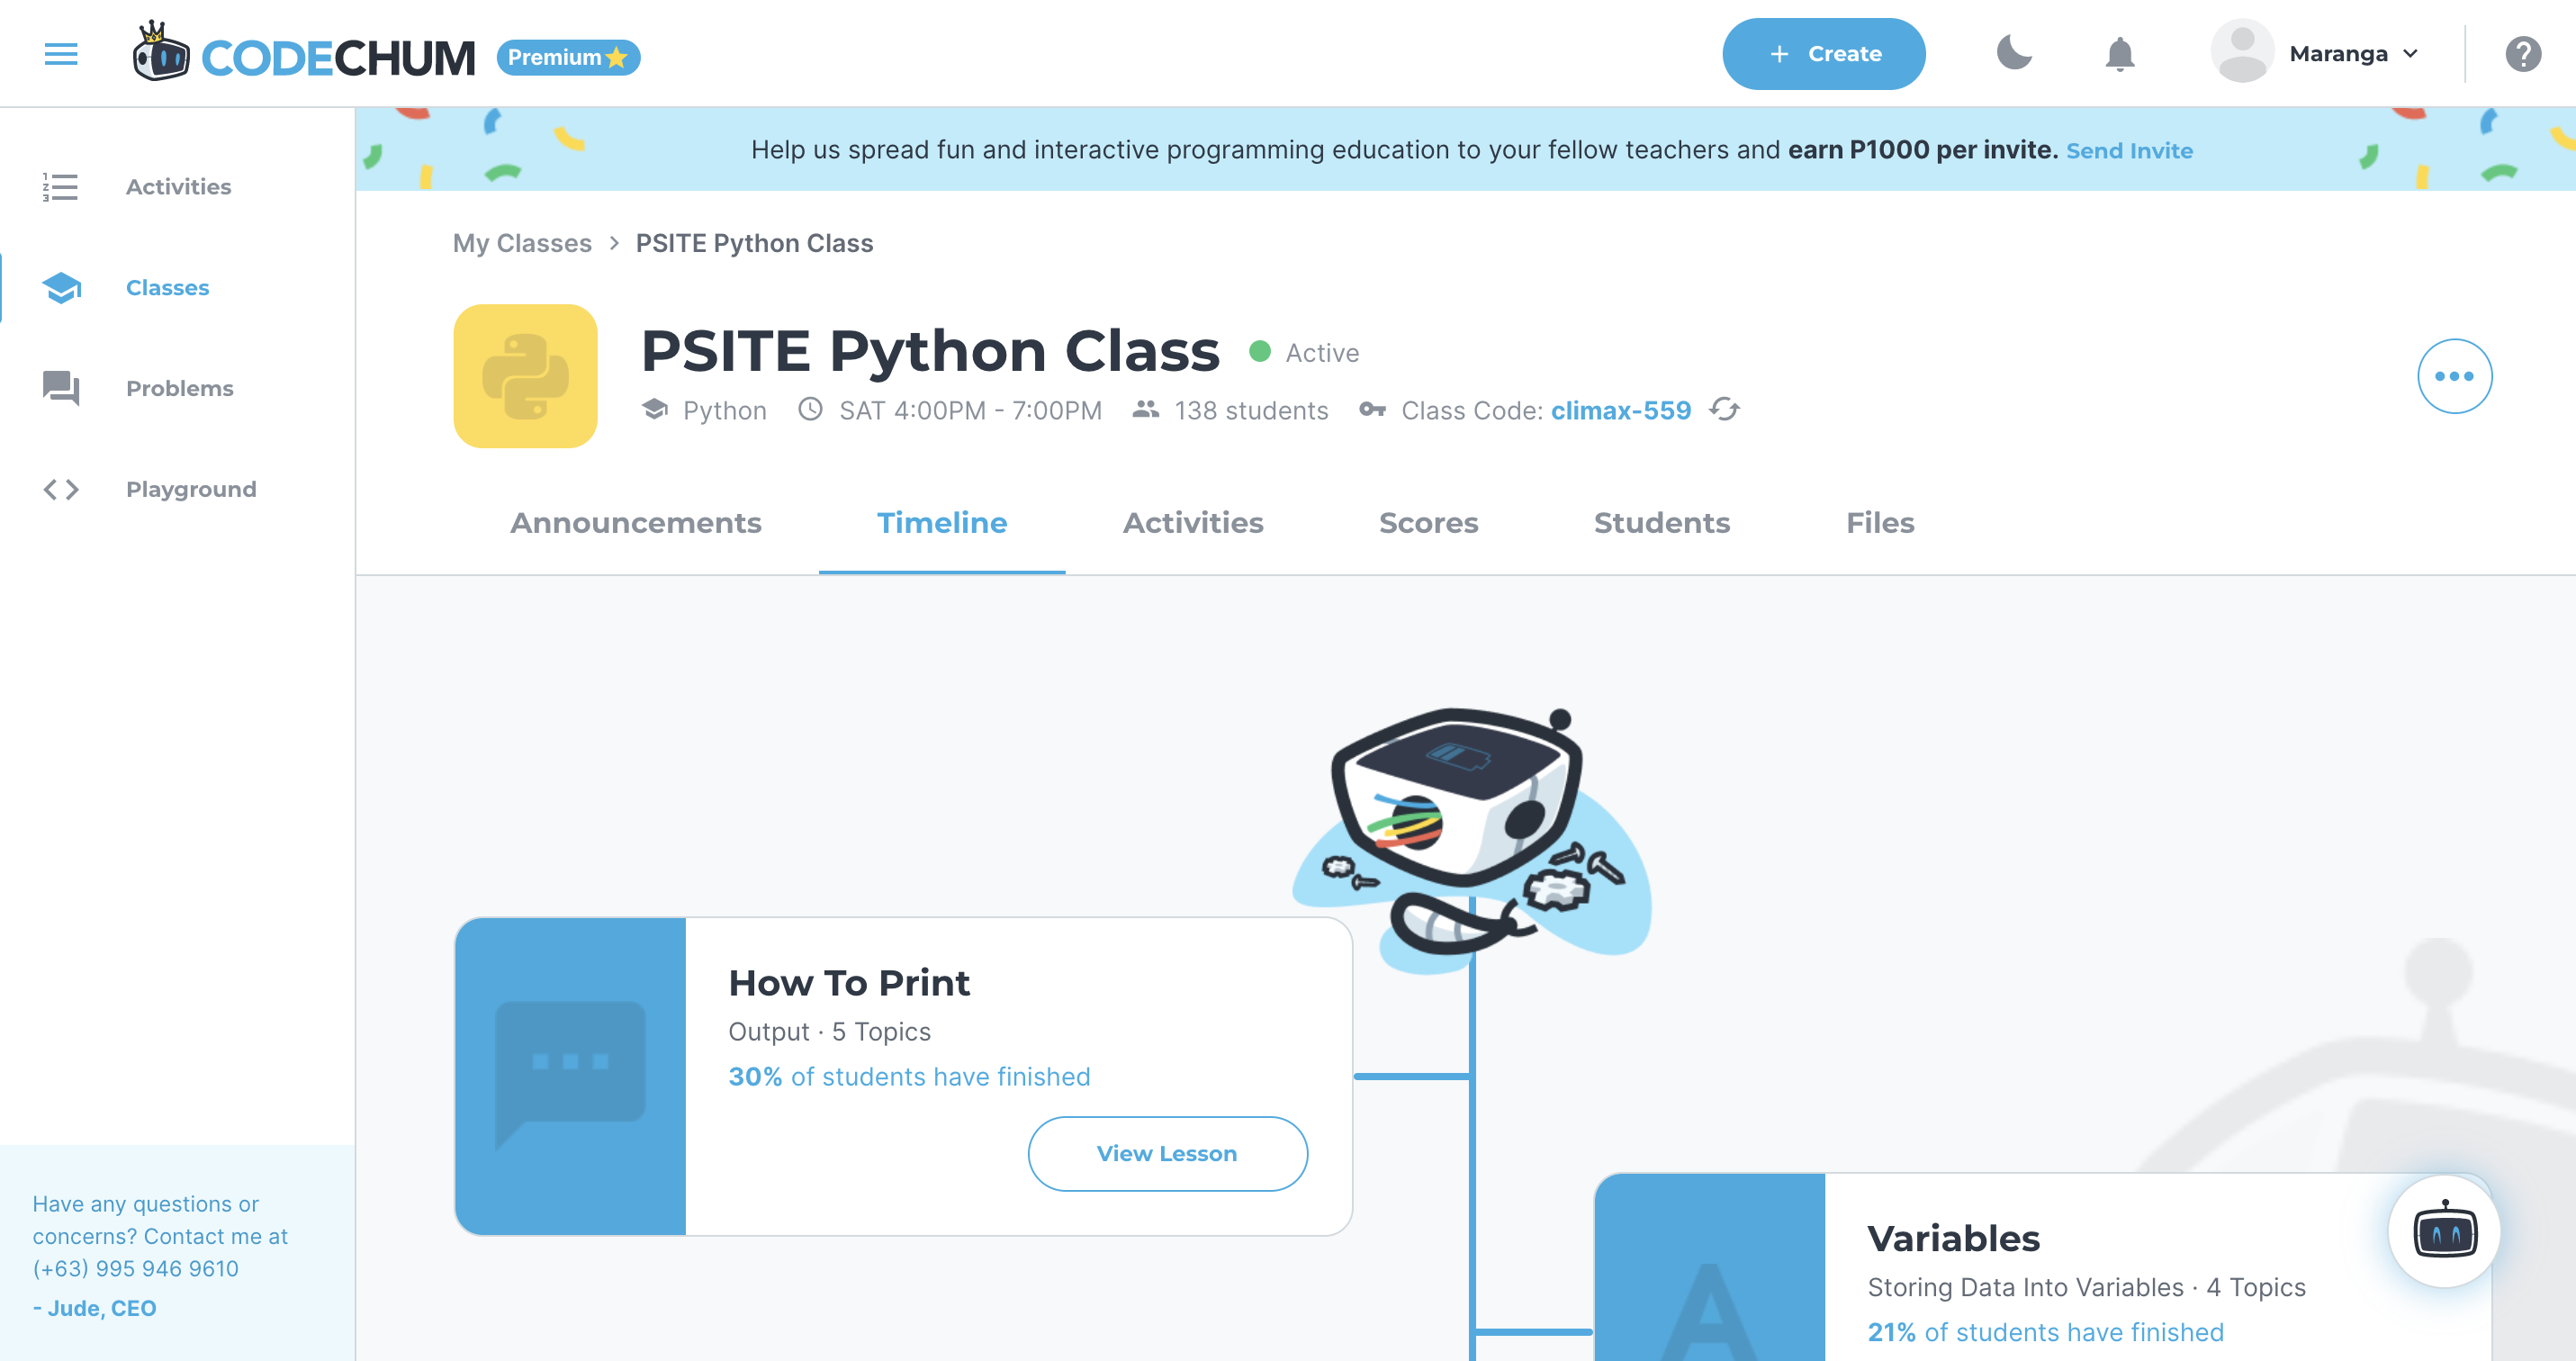
\includegraphics[width=\textwidth]{images/CodeChum UI.png}
	\caption{
		Sučelje \textit{web} aplikacije CodeChum.
	}
	\label{fig:codechum-ui}
\end{figure}

\textit{Web} aplikacije poput HackerRank \citep{HackerRank}, TestDome \citep{TestDome} i Filtered \citep{Filtered} koriste se u regrutaciji i procesu zapošljavanja novih softverskih inženjera. Nakon što se prijave na otvorenu poziciju, kandidatima se automatski šalje elektronička pošta s uputama za rješavanje programskih zadataka. Zadatke koje će kandidat rješavati priprema tvrtka za čiju poziciju se kandidat natječe, a težina i vrsta zadataka ovisi o otvorenoj poziciji. Aplikacije za regrutaciju i automatizaciju procesa zapošljavanja najčešće nude svoju biblioteku zadataka koje tvrtke mogu odabrati prilikom izrade ispita za pojedini natječaj. Ovakve \textit{web} aplikacije korisne su tvrtkama koje svakodnevno dobivaju preveliku količinu prijava koje odjel za ljudske resurse može pogledati, stoga im automatizirano ispitivanje kandidata pomaže u inicijalnom filtriranju  prilikom zapošljavanja. Osim filtriranja kandidata ove \textit{web} aplikacije pomažu i pri provođenju \textit{online} razgovora gdje kandidati svoje vještine rješavanja problemskih zadatka trebaju pokazati pred ispitivačem koji vodi razgovor (slika \ref{fig:hackerrank-ui}).

\begin{figure}[htb]
	\centering
	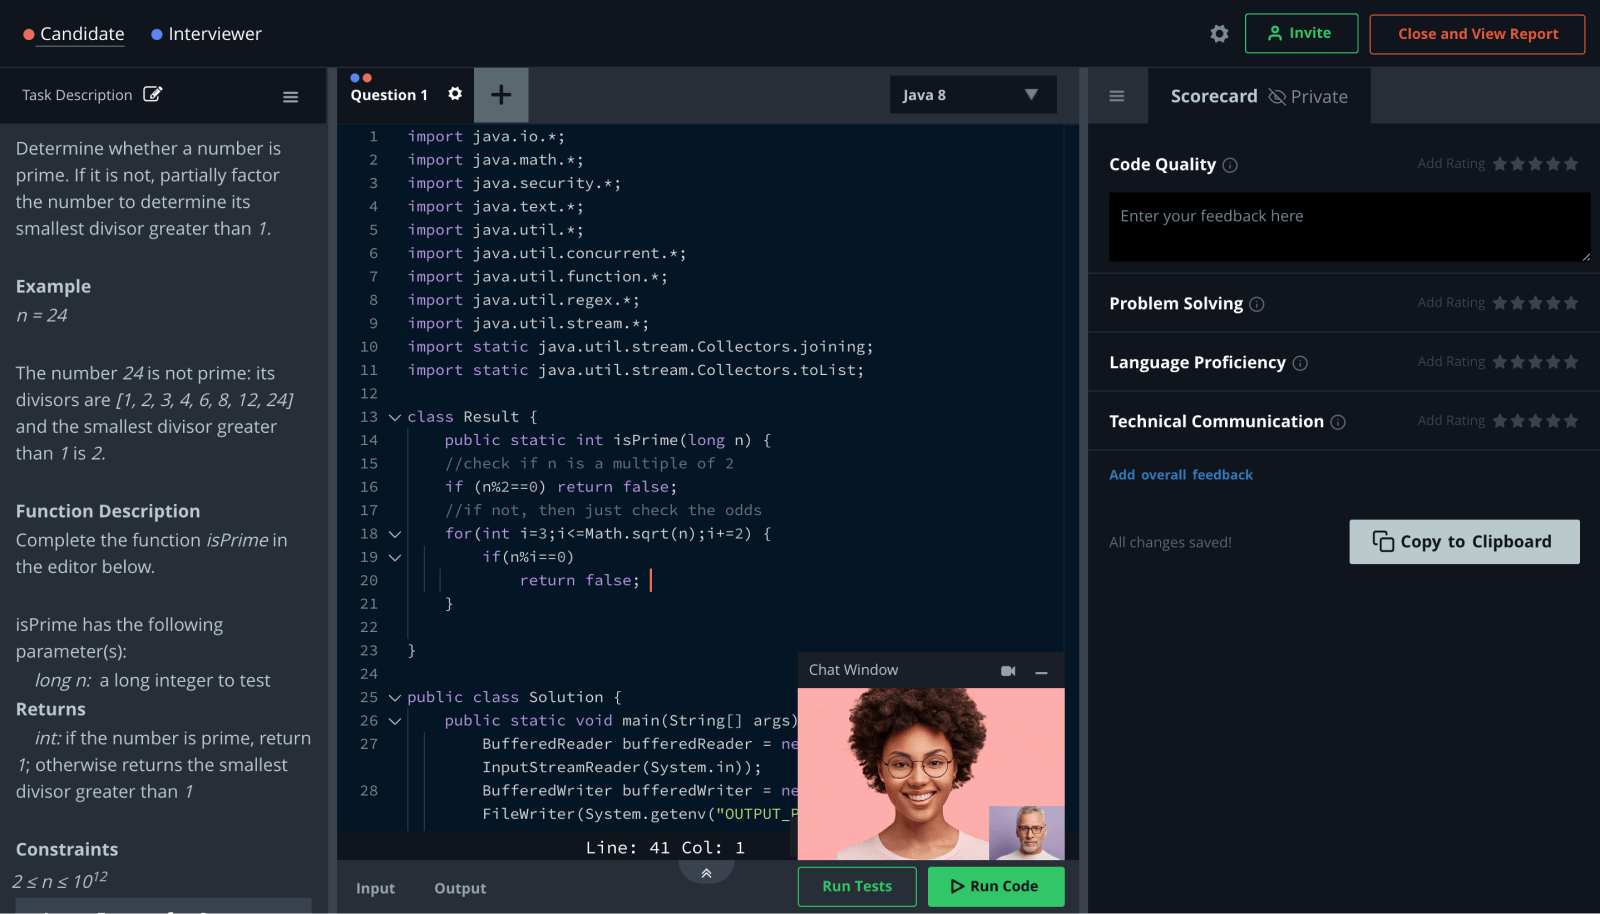
\includegraphics[width=\textwidth]{images/HackerRank UI.png}
	\caption{
		Sučelje \textit{web} aplikacije HackerRank. \citep{HackerRank}
	}
	\label{fig:hackerrank-ui}
\end{figure}

Osim što pomažu u regrutaciji i procesu zapošljavanja, sustavi za udaljeno ocjenjivanje dolaze i u izvedbi kao \textit{web} aplikacije za vježbanje i pripremu za razgovore za posao koji uključuju rješavanje problemskih zadataka. \textit{Web} aplikacije poput: AlgoExpert \citep{AlgoExpert}, AlgoDaily \citep{AlgoDaily} i LeetCode \citep{LeetCode} svojim korisnicima nude bogatu biblioteku problemskih zadataka, njihovih rješenja i mnogo sadržaja za učenje algoritama i struktura podataka, a sve u svrhu kvalitetne pripreme za tzv. \textit{coding interview}.

\begin{figure}[htb]
	\centering
	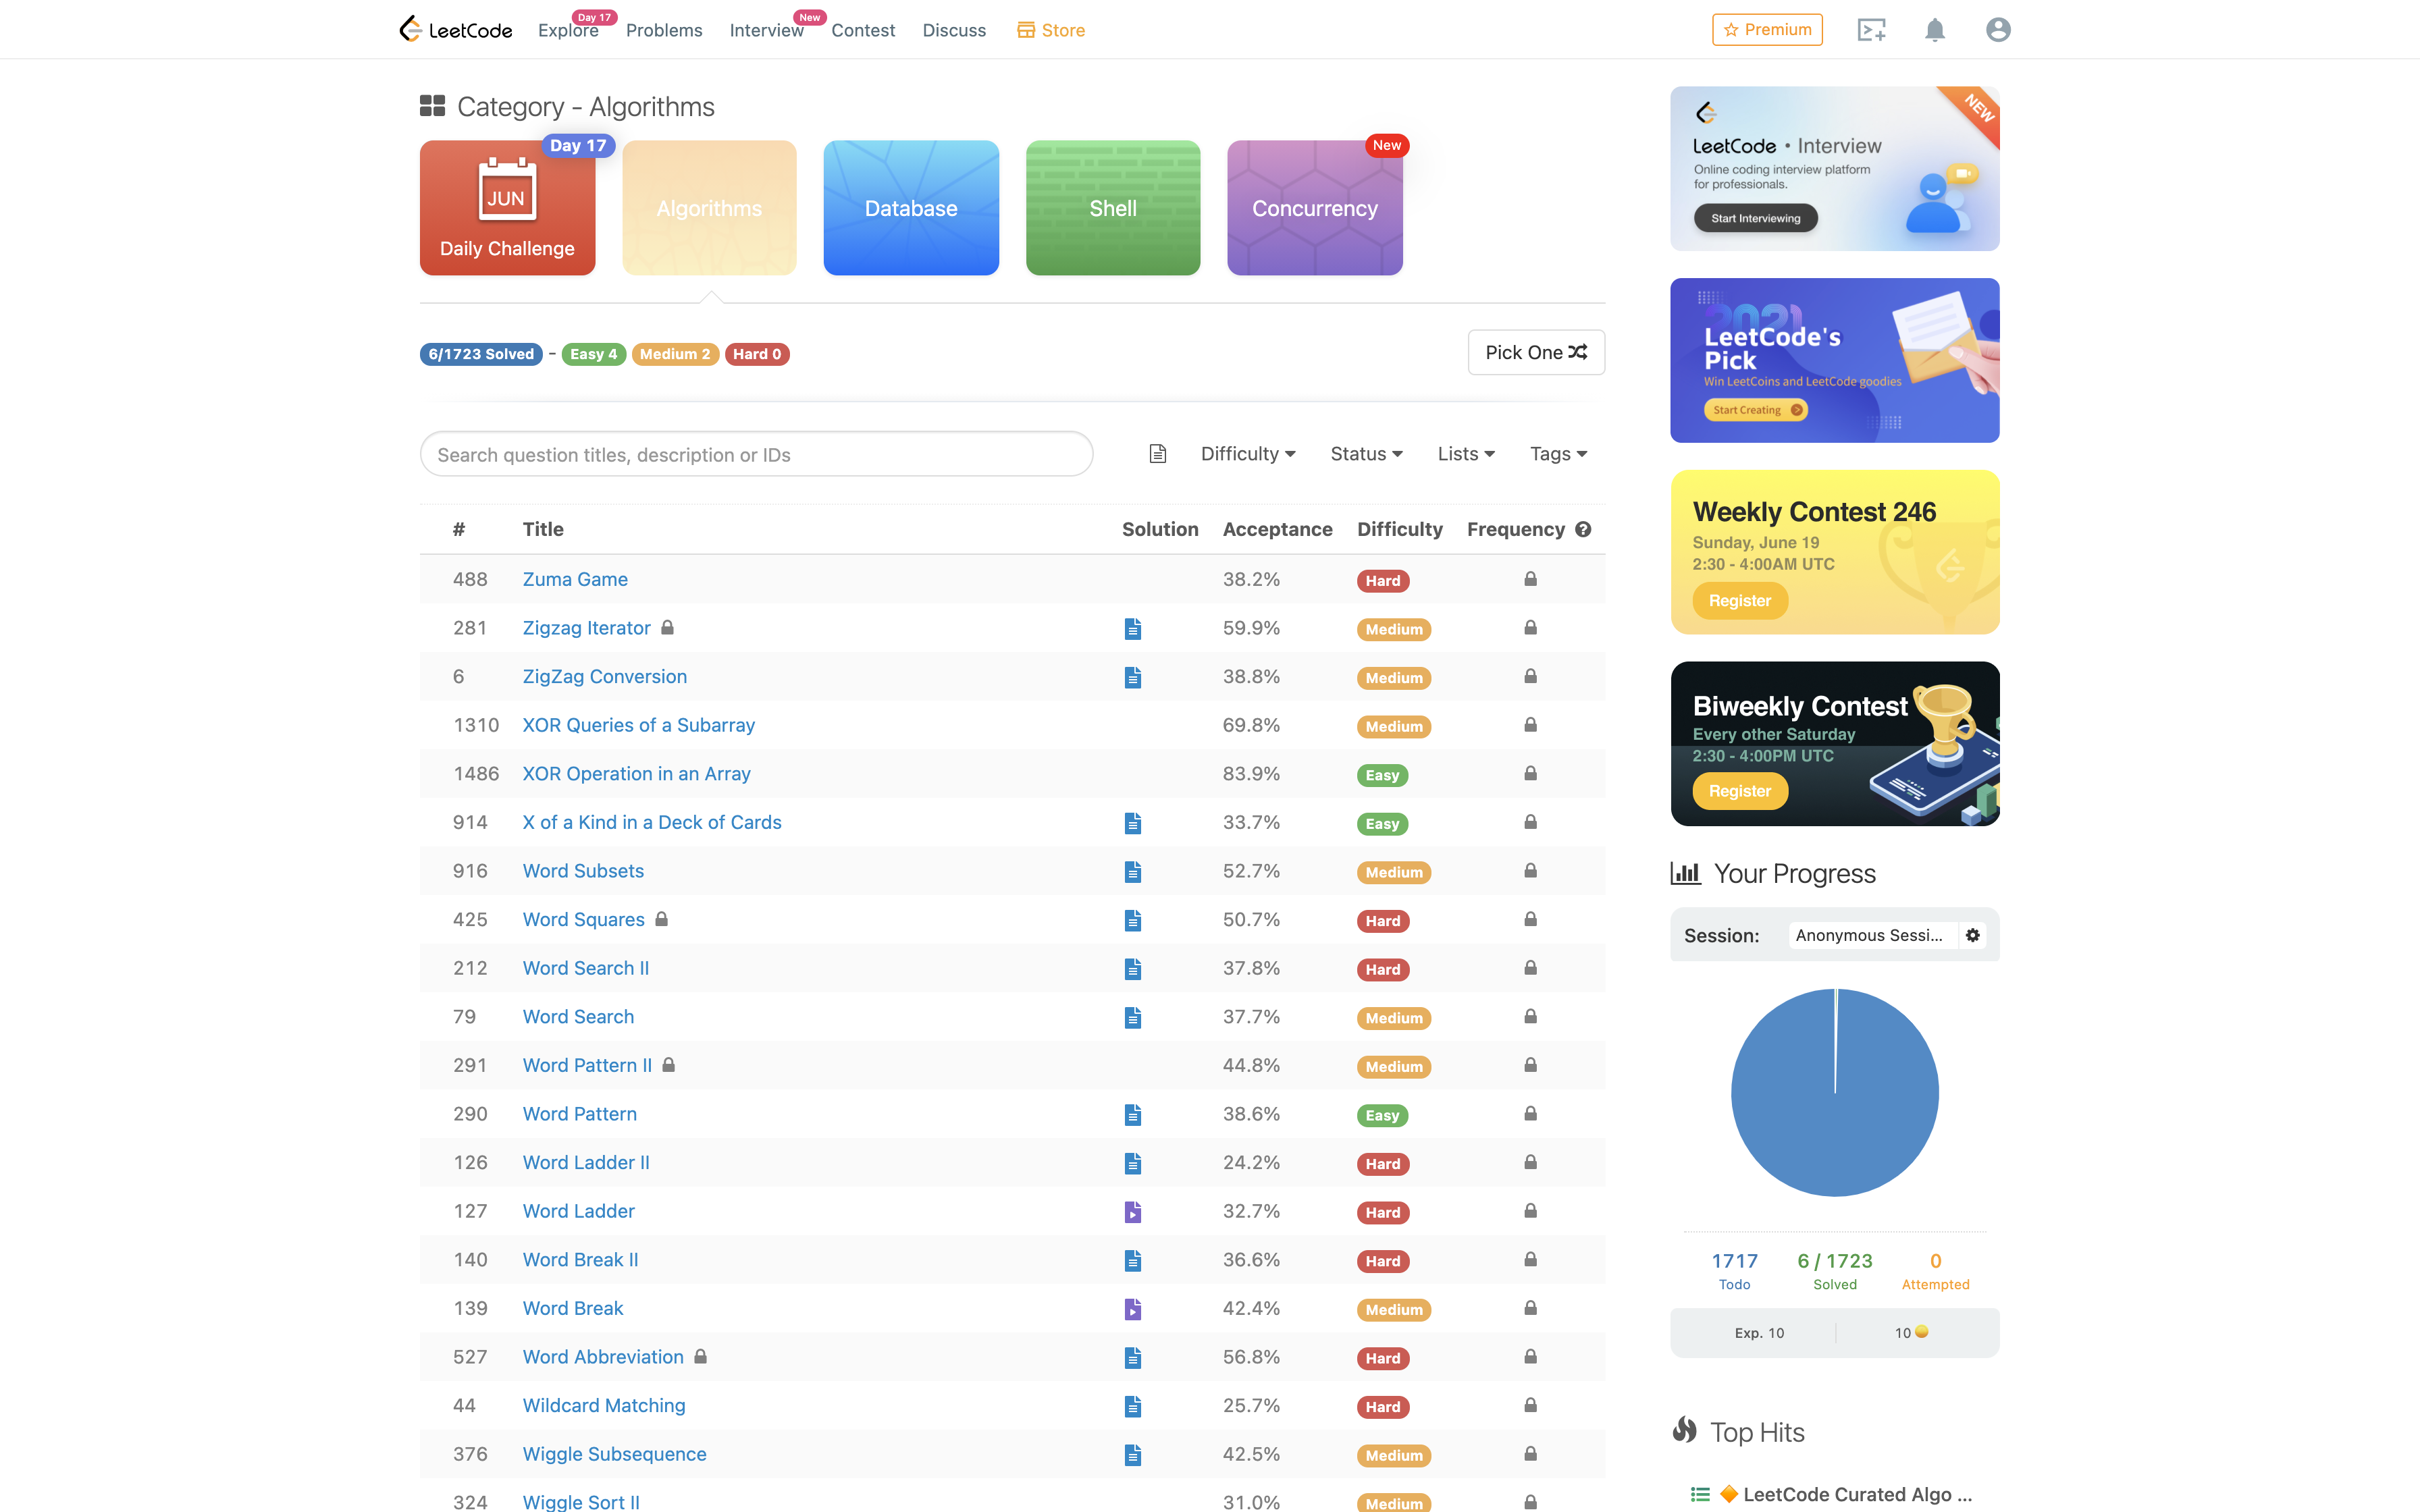
\includegraphics[width=\textwidth]{images/LeetCode UI.png}
	\caption{
		Sučelje \textit{web} aplikacije LeetCode.
	}
	\label{fig:leetcode-ui}
\end{figure}

\chapter{Analiza performansi sustava za udaljeno izvršavanje programskog kôda}
\label{chap:analysis}
Analiza performansi sustava za udaljeno izvršavanje programskog kôda ne spominje se u literaturi budući da se tek od \citep{9245310} sustavi za udaljeno izvršavanje programskog kôda razmatraju kao zasebne komponente u arhitekturi sustava za udaljeno ocjenjivanje. U radu \citep{drung2011enhance} razmatra se optimizacija performansi postojećeg sustava za udaljeno ocjenjivanje, međutim, ono je usmjereno na ugađanje opcija operacijskog sustava i algoritama raspoređivanja zahtjeva za izvršavanje.

Ovaj rad predstavlja prvi radni okvir za analizu performansi i ocjenu kvalitete i pouzdanosti (u daljnjem tekstu: \textit{radni okvir}) usluge sustava za udaljeno izvršavanje programskog kôda (u daljnjem tekstu: \textit{sustav}). Prema \citep{nidhra2012black} ovakva vrsta analize u spektru testiranja softvera naziva se \textit{system testing}, a proučava kako sustav funkcionira u produkcijskom okruženju iz perspektive korisnika. Također, prema uvidu u sustav koji se testira, ovakva vrsta testiranja naziva se \textit{black box testing}.

Za analizu performansi i ocjenu kvalitete i pouzdanosti pojedinog sustava potrebno je promatrati rad sustava s različitim dinamikama višekorisničkog opterećenja, različitim scenarijima korištenja i različitim načinima interakcije sa sustavom. To su dimenzije po kojima možemo promatrati rad sustava, i njihov opis slijedu u nastavku ovog poglavlja.

\section{Dinamike višekorisničkog opterećenja}
Budući da sustav za udaljeno izvršavanje programskog kôda neposredno preko sustava za udaljeno ocjenjivanje koristi više krajnjih korisnika istovremeno, u analizi performansi potrebno je razmatrati višekorisničko opterećenje.

Radni okvir omogućuje razmatranje tri različite dinamike višekorisničkog opterećenja koje se koriste prilikom stvaranja zahtjeva za izvršavanje programskog kôda (u nastavku teksta: \textit{zahtjevi}):
\begin{itemize}
    \item impulsno-determinističko opterećenje,
    \item kontinuirano-determinističko opterećenje, i
    \item kontinuirano-stohastičko opterećenje.
\end{itemize}

Svaka vrsta višekorisničkog opterećenja detaljno je opisana u nastavku ove cjeline. 

\subsection{Impulsno-determinističko opterećenje sustava}
\label{subsec:id-load}
Impulsno-determinističko opterećenje sustava definirano je parametrima $N$ i $M$, gdje $N$ predstavlja broj zahtjeva koje treba istovremeno poslati, dok $M$ predstavlja broj iteracija koje je potrebno napraviti uz ogradu da zahtjevi poslani u iteraciji $i$ smiju biti poslani tek nakon što se izvrše zahtjevi u iteraciji $i - 1$. U svakoj od $M$ iteracija poslat će se $N$ istovremenih zahtjeva, odnosno, na kraju eksperimenta očekujemo da je u sustav pristiglo sveukupno $N \times M$ zahtjeva.

\begin{figure}[htb]
	\centering
	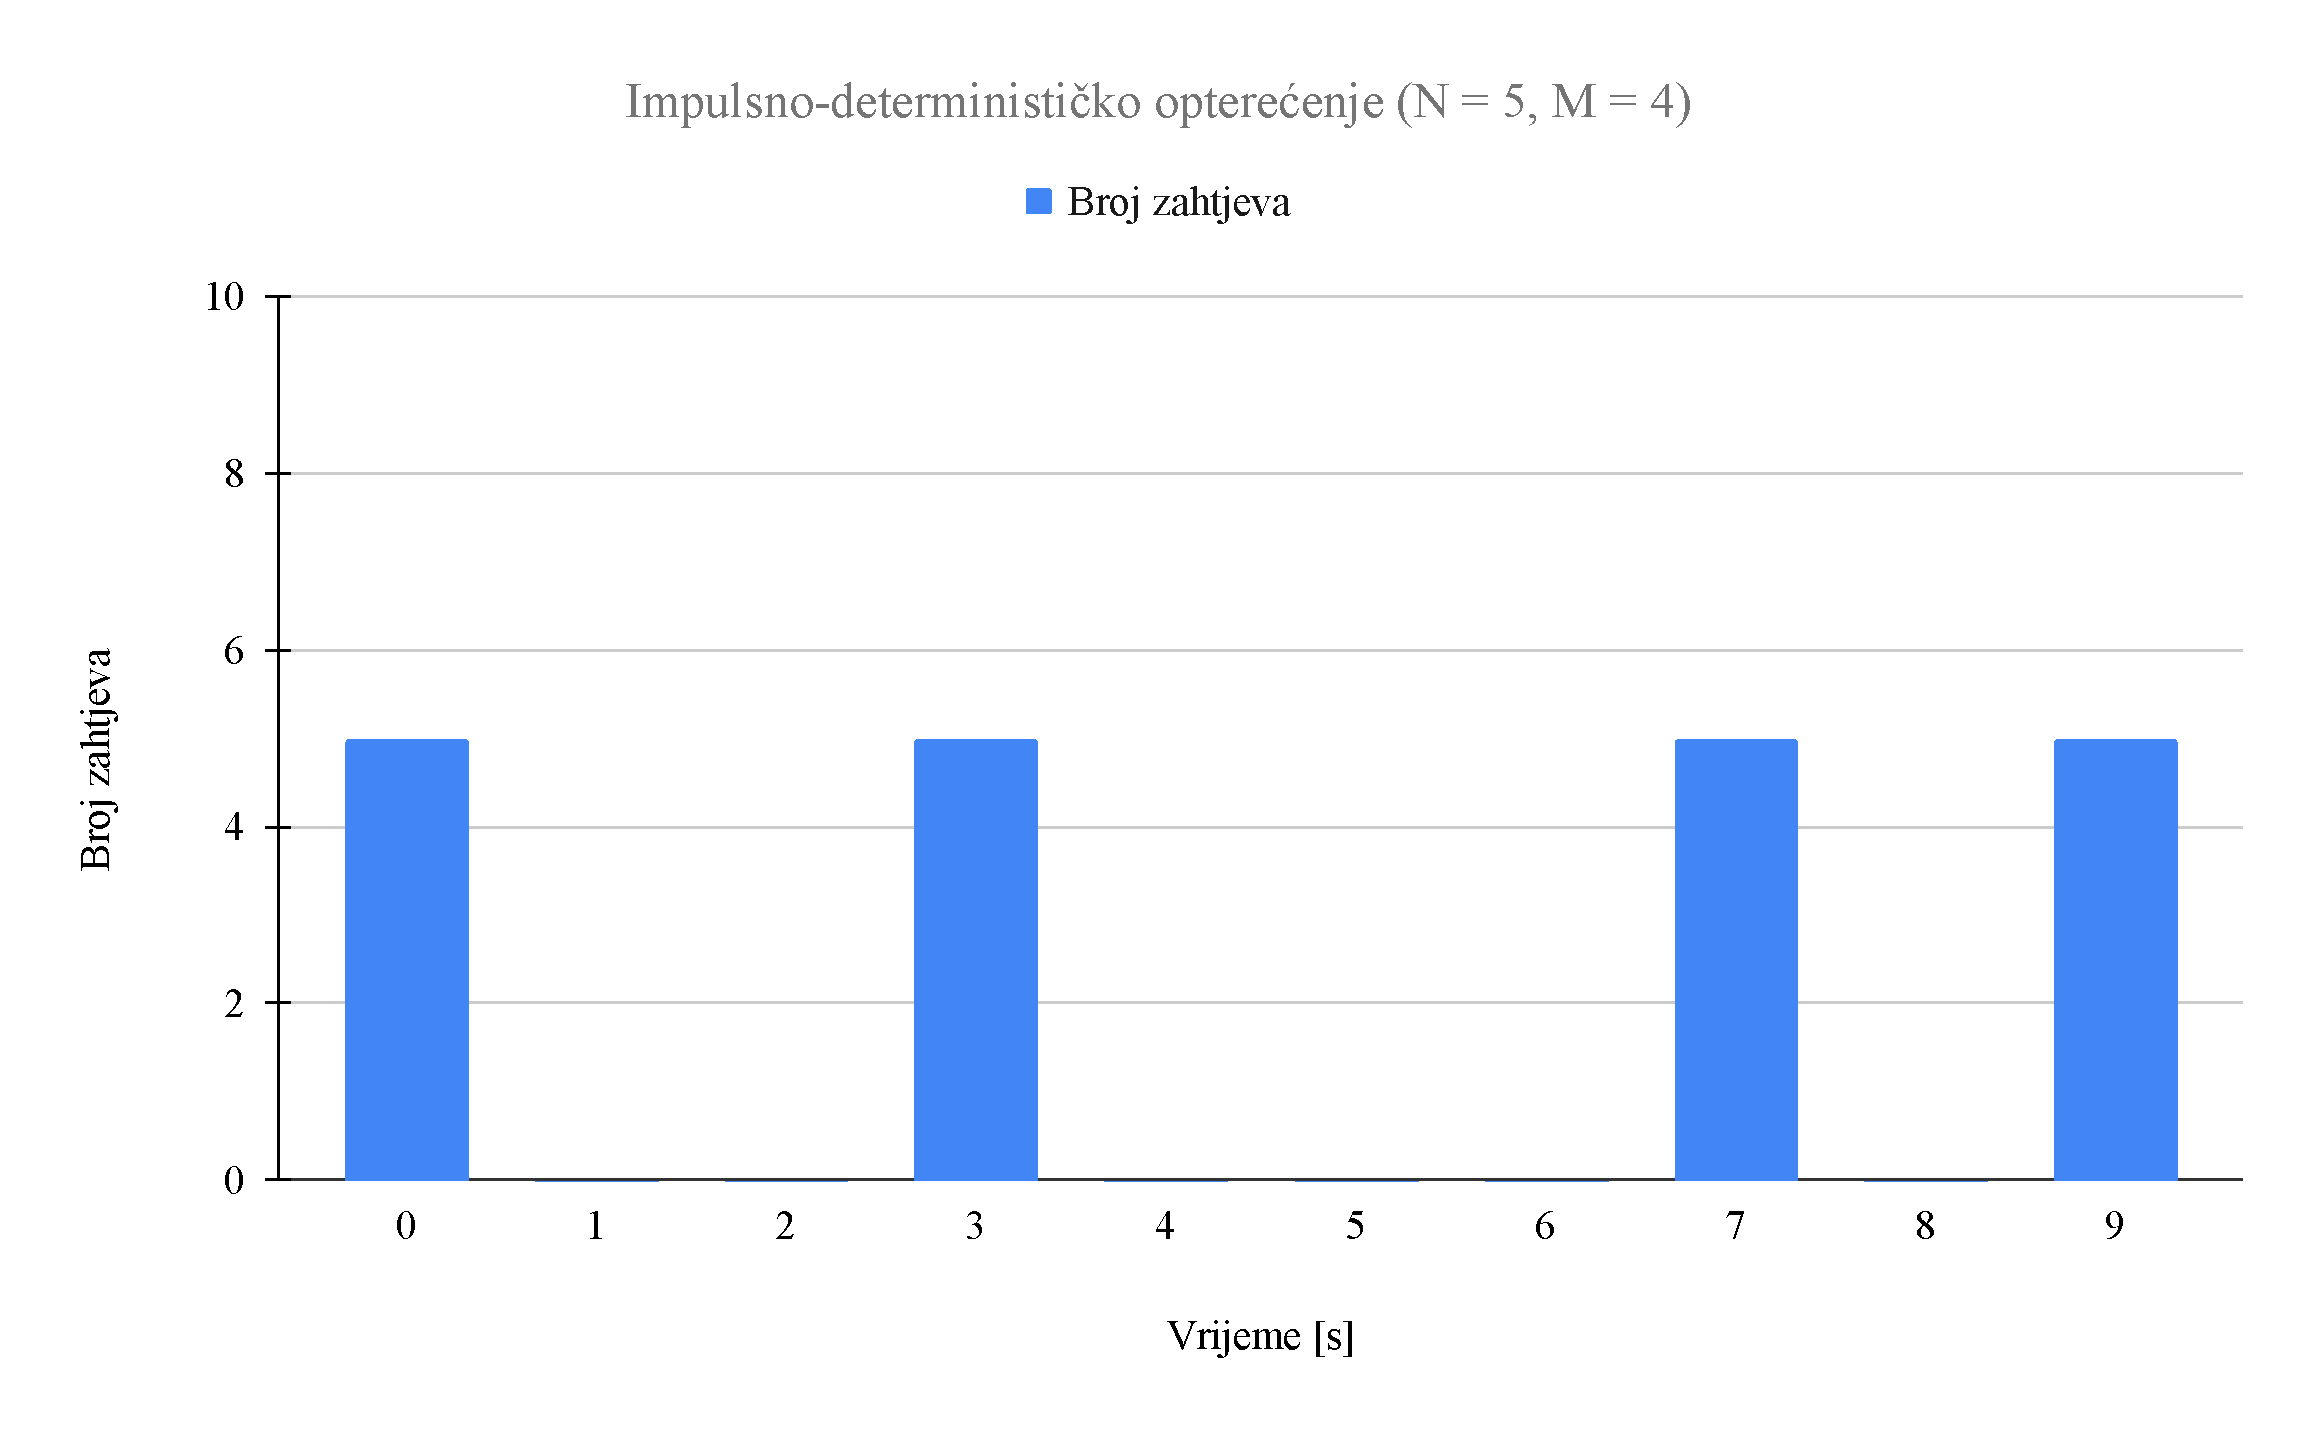
\includegraphics[width=\textwidth]{images/Impulsno-deterministicko opterecenje (N = 5, M = 4).pdf}
	\caption{
		Impulsno-determinističko opterećenje sustava (N = 5, M = 4).
	}
	\label{fig:id-load}
\end{figure}

Slika \ref{fig:id-load} prikazuje primjer dinamike impulsno-determinističkog opterećenja sustava s 5 istovremenih zahtjeva kroz 4 iteracije. U trenutku $t=0$ započinje slanje prvih 5 zahtjeva koje je sustav obrađuje do trenutka $t=3$ kada započinje slanje idućih 5 zahtjeva itd. Primjer na slici \ref{fig:id-load} također pokazuje da iako se u svakoj iteraciji šalje ista količina zahtjeva to ne znači nužno da će sustavu trebati isti vremenski period da ih obradi.

Impulsno-determinističko opterećenje sustava predstavlja najjednostavniju dinamiku opterećenja sustava, međutim, takva dinamika ne oponaša stvarno produkcijsko okruženje.

\subsection{Kontinuirano-determinističko opterećenje sustava}
\label{subsec:cd-load}
Kontinuirano-determinističko opterećenje sustava definirano je također parametrima $N$ i $M$, međutim, za razliku od prethodne vrste opterećenja, istovremeni zahtjevi u iteraciji $i$ smiju biti poslani i prije nego što se izvrše zahtjevi u iteraciji $i-1$, ali tek u vremenu $t_i = t_{i - 1} + 1$, gdje je vrijeme $t$ izraženo u sekundama. Budući da pri intenzivnom višekorisničkom opterećenju vrijeme obrade zahtjeva može trajati i po nekoliko desetaka sekundi, korak od jedne sekunde predstavlja najmanji interval vremena koji ima smisla promatrati kada se govori o broju zahtjeva koji dolaze u sustav po jedinici vremena.

Slika \ref{fig:cd-load} prikazuje primjer dinamike kontinuirano-determinističkog opterećenja od 10 iteracija gdje je u svakoj iteraciji napravljeno 5 zahtjeva.

\begin{figure}[htb]
	\centering
	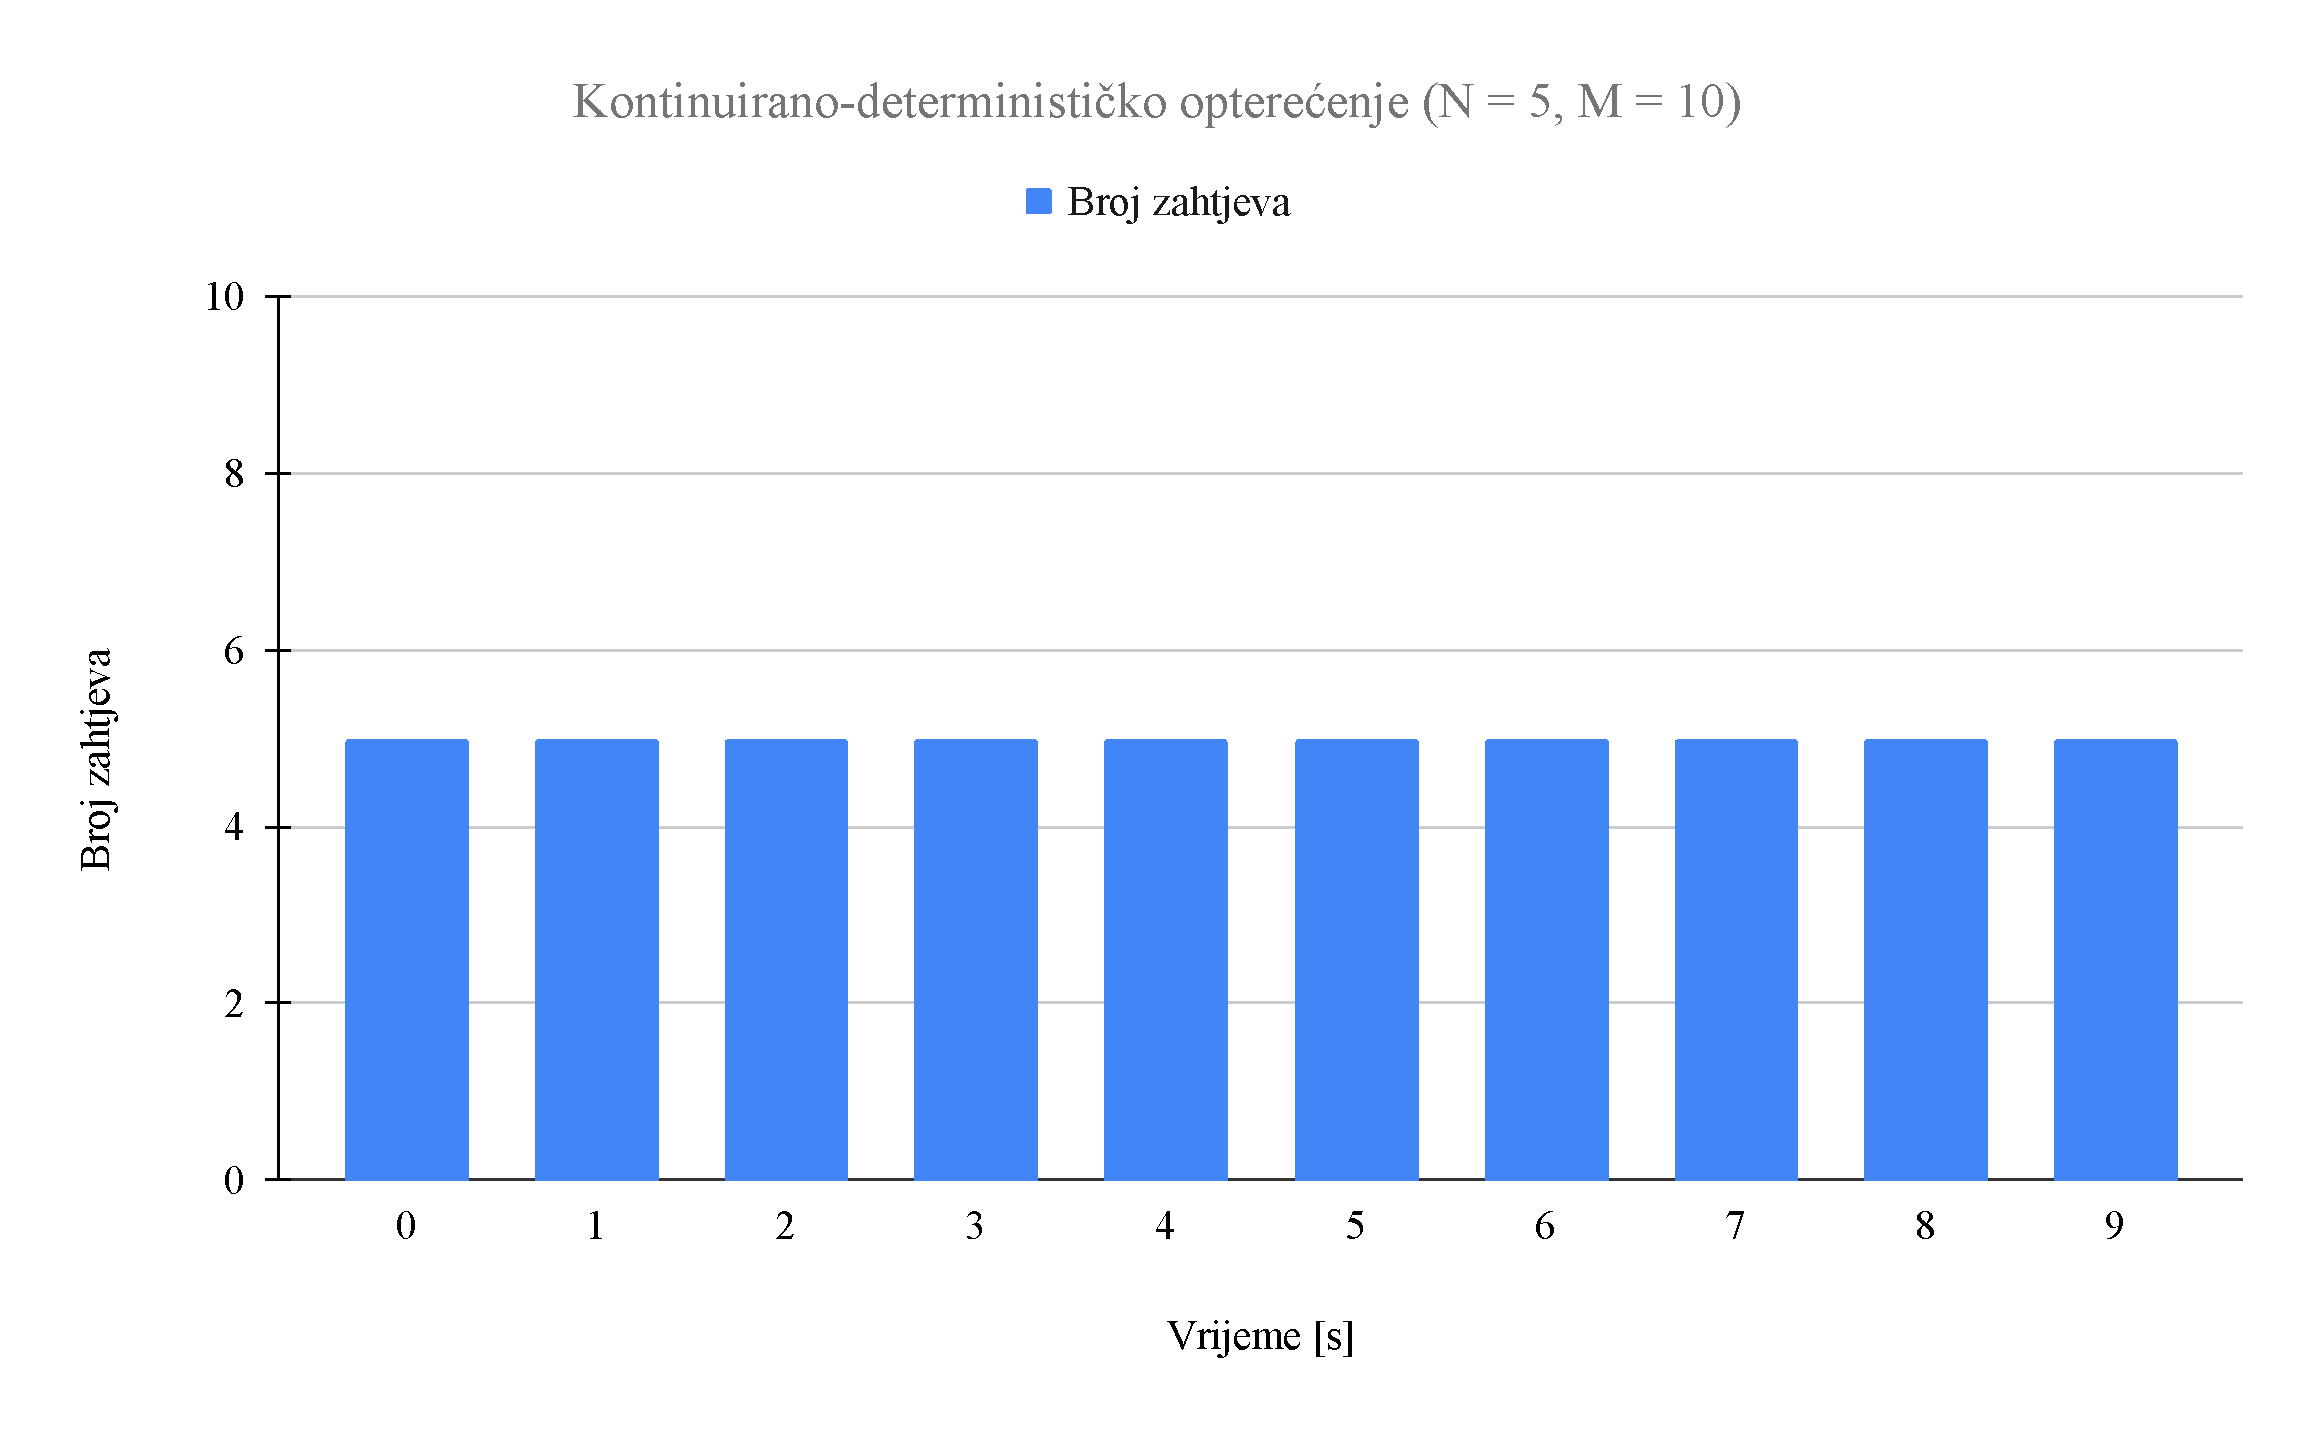
\includegraphics[width=\textwidth]{images/Kontinuirano-deterministicko opterecenje (N = 5, M = 10).pdf}
	\caption{
		Kontinuirano-determinističko opterećenje sustava (N = 5, M = 10).
	}
	\label{fig:cd-load}
\end{figure}

\pagebreak

\subsection{Kontinuirano-stohastičko opterećenje sustava}
Za razliku od kontinuirano-determinističkog opterećenja koje u svakom koraku $i$ koristi nepromjenjivi $N$, kontinuirano-stohastičko opterećenje sustava koristi Poissonovu distribuciju s parametrom $\lambda = N$ za određivanje broja istovremenih zahtjeva u koraku $i$. Slika \ref{fig:cs-load} prikazuje primjer dinamike kontinuirano-stohastičkog opterećenja s parametrima $N=5$ i $M=10$. Niz pseudo-slučajnih brojeva iz primjera generiran je pomoću isječka \ref{lst:poisson-numbers} napisanog u programskom jeziku Python.

\

\begin{lstlisting}[
    caption={Generiranje pseudo-slučajnih brojeva iz Poissonove distribucije.},
    label={lst:poisson-numbers},
    language=python
]
import numpy
N, M = 5, 10
print(numpy.random.poisson(N, M))
\end{lstlisting}

Kontinuirano-stohastičko opterećenje sustava najbliže oponaša stvarnu dinamiku korištenja sustava prilikom višekorisničkog opterećenja. Parametrom $N$ regulira se prosječan broj korisnika u sekundi, dok se parametrom $M$ regulira duljina trajanja opterećenja.

\begin{figure}[htb]
	\centering
	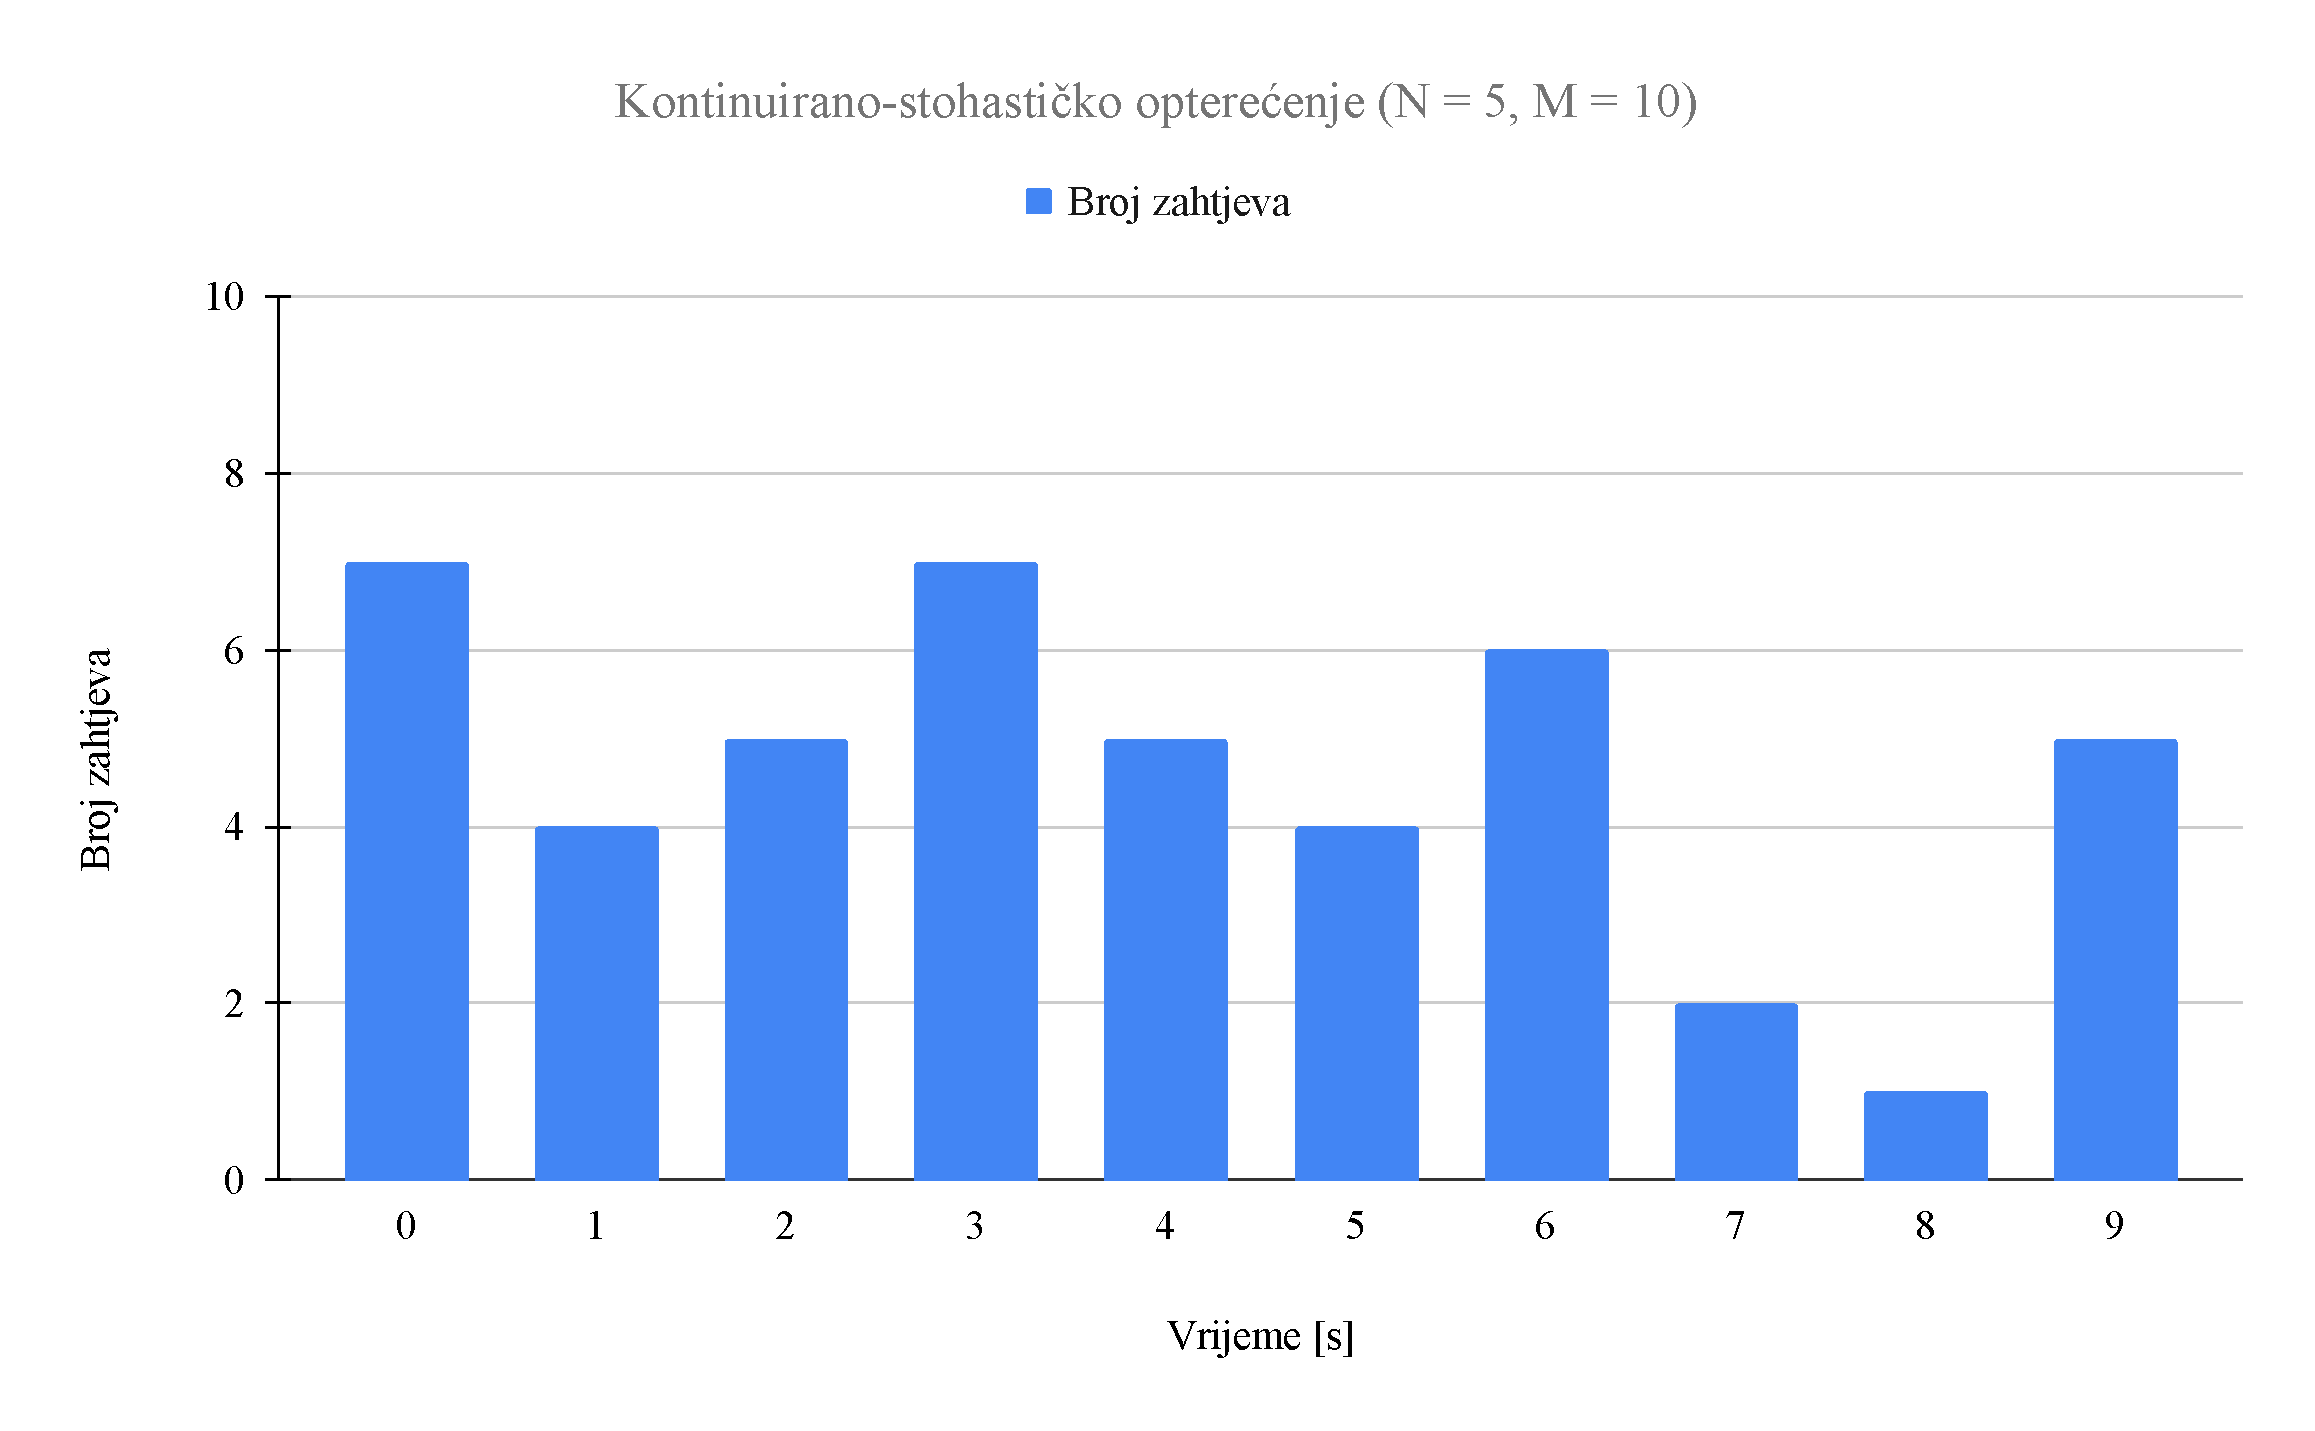
\includegraphics[width=\textwidth]{images/Kontinuirano-stohasticko opterecenje (N = 5, M = 10).pdf}
	\caption{
		Kontinuirano-stohastičko opterećenje sustava (N = 5, M = 10).
	}
	\label{fig:cs-load}
\end{figure}

\pagebreak

\section{Scenariji korištenja i programski jezici}
Nakon odabira dinamike višekorisničkog opterećenja potrebno je odabrati scenarij korištenja i programski jezik. U produkcijskom okruženju nemoguće je predvidjeti koji programski kôd će sustav trebati izvršiti, međutim, programski kôdovi koji pristižu u sustav mogu se podijeliti u četiri scenarija korištenja:
\begin{itemize}
    \item[$\bullet$] jednostavan scenarij,
    \item[$\bullet$] scenarij procesorskog opterećenja,
    \item[$\bullet$] scenarij mrežnog opterećenja, i
    \item[$\bullet$] scenarij procesorskog i mrežnog opterećenja.
\end{itemize}

Svaki scenarij pažljivo je odabrani zadatak koji treba riješiti, međutim, za razliku od uobičajenih zadataka, scenarij također daje i uputu na koji način zadatak treba riješiti. Ova ograda važna je da bi se mogla raditi analiza između dva različita scenarija. Tako se npr.\ uz pažljivo odabrane scenarije mogu uspoređivati scenarij procesorskog opterećenja, i scenarij procesorskog i mrežnog opterećenja ako i samo ako se zna da je drugi zaista mrežno opterećena inačica prvog.

Prilikom analize pretpostavlja se da su programski kôdovi scenarija ispravni, odnosno da se mogu uspješno prevesti i izvesti u svakom sustavu koji se promatra. Ova pretpostavka uspješnosti prevođenja i izvršavanja ključna je u analizi budući da pri intenzivnom višekorisničkom opterećenju može doći do preopterećenja sustava koje rezultira npr. neuspješnim prevođenjem zbog manjka radne memorija.

Implementacija svakog scenarija korištenja dostupna je u tri programska jezika: \text{C++}, Java i Python. Iako se u okviru ovog rada promatraju samo navedeni programski jezici, radni okvir analize nije ograničen samo na njih. Također, u ovom radu ne razmatraju se višedretvene implementacije scenarija.

Svaki scenarij sastoji se od: standardnog ulaza, programskog kôda i očekivanog standardnog izlaza. Standardni ulaz i očekivani standardni izlaz isti su za svaki programski jezik u kojem je scenarij implementiran. Sadržaj standardnog ulaza dovodi se na ulaz programa koji je nastao prevođenjem programskog kôda scenarija u odabranom programskom jeziku, a očekivani standardni izlaz koristi se za usporedbu sa standardnim izlazom programa nakon njegovog izvršavanja. Ova provjera važna ja kako bi se utvrdilo da je program zaista odradio zadatak zadan scenarijem.

\subsection{Jednostavan scenarij}
Jednostavan scenarij zahtjeva da korisnički program ispiše \lstinline{hello, world} na standardni izlaz.

Jednostavan scenarij predstavlja najjednostavniji smisleni programski kôd koji korisnik može izvesti putem sustava. Ovaj scenarij također predstavlja minimalno mrežno, procesorsko i memorijsko opterećenje na poslužitelju sustava.

Vremenska i memorijska složenost algoritma koji implementira rješenje ovog scenarija je $\mathcal{O}(1)$.

\subsection{Scenarij procesorskog opterećenja}
Scenarij procesorskog opterećenja zahtjeva ispis medijana od 20.000 cijelih brojeva tipa \textit{integer} koji se na standardni ulaz dovode silazno sortirani. Scenarij također zahtjeva da se pročitanih 20.000 brojeva najprije uzlazno sortira mjehurićastim sortiranjem \engl{bubble sort}.

Vremenska složenost algoritma koji implementira rješenje ovog scenarija je $\mathcal{O}(n^2)$, a memorijska složenost je $\mathcal{O}(n)$, gdje je $n$ duljina ulaznog niza brojeva.

Odabir 20.000 za duljinu ulaznog niza brojeva i zahtjev da brojevi budu sortirani suboptimalnim algoritmom mjehurićastog sortiranja nije slučajan, nego pažljivo odabran budući da vrijeme izvođenja programa koji implementira rješenje tog scenarija traje zamjetno dulje od jednostavnog scenarija. Konkretno, na procesoru Intel Core i7 radnog takta 2,6 GHz računala MacBook Pro (16-inch, 2019) \text{C++} implementacija rješenja ovog scenarija traje oko 2,5 sekundi.

Ulazni niz brojeva koji se na standardni ulaz dovode silazno sortirani odabran je zato što predstavlja najgori mogući slučaj \engl{worst case} za algoritam mjehurićastog sortiranja koji brojeve treba sortirati uzlazno.

\subsection{Scenarij mrežnog opterećenja}
Scenarij mrežnog opterećenja očekuje da program ispiše sumu 750.000 cijelih brojeva tipa \textit{integer} koji se na standardni ulaz dovode silazno sortirani.

Mrežno opterećenje ovog scenarija očituje se u veličini sadržaja standardnog ulaza u iznosu od 5,1 MB.

Vremenska i memorijska složenost algoritma koji implementira rješenje ovog scenarija je $\mathcal{O}(n)$, gdje je $n$ duljina ulaznog niza brojeva.

\subsection{Scenarij procesorskog i mrežnog opterećenja}
Scenarij procesorskog i mrežnog opterećenja spoj je prethodna dva scenarija. Ovaj scenarij zahtjeva da program ispiše medijan prvih 20.000 brojeva iz niza od 750.000 brojeva koji se na standardni ulaz dovode silazno sortirani. Također, kao i u scenariju procesorskog opterećenja, od programa se očekuje da brojeve sortira suboptimalnim algoritmom mjehurićastog sortiranja.

Standardni ulaz ovog scenarija isti je kao i standardni ulaz scenarija mrežnog opterećenja, i algoritam rješenja ovog scenarija isti je kao algoritam rješenja scenarija procesorskog opterećenja.

Vremenska složenost algoritma koji implementira rješenje ovog scenarija je $\mathcal{O}(n^2)$, a memorijska složenost je $\mathcal{O}(n)$, gdje je $n$ duljina ulaznog niza brojeva, uz ogradu da $n$ ne može biti veći od 20.000.

\section{Strategije izvršavanja}
Odabir strategije izvršavanja programskog kôda svodi se na odabir načina interakcije sa sustavom koji su objašnjeni u pododjeljku \ref{subsec:interaction}.

Bilo da se radi o sinkronoj ili asinkronoj interakciji prvi zahtjev prema sustavu naziva se \textit{zahtjev narudžbe} \engl{order request} koji sadrži sve potrebne informacije koje sustav treba za izvršavanje programskog kôda, a to su: programski kôd, identifikator programskog jezika, standardni ulaz i očekivani standardni izlaz.

Ako se koristi sinkrona interakcija sa sustavom onda će odgovor na zahtjev narudžbe biti rezultat izvršavanja programskog kôda. 

Međutim, ako se koristi asinkrona interakcija tada je potrebno raditi tzv. \textit{zahtjev ispitivanja} \engl{probe request} tako dugo dok se ne utvrdi da je izvršavanje završilo. Implementacija radnog okvira u aplikaciji Hélory radi jedan zahtjev ispitivanja po sekundi s time da između zahtjeva narudžbe i prvog zahtjeva ispitivanja mora proći dvije sekunde. Ova dinamika slanja zahtjeva ispitivanja odabrana je jer ju sustav Sphere Engine preporuča u svojoj dokumentaciji.

Sustav Piston podržava sinkronu strategiju izvršavanja, sustav Sphere Engine asinkronu, a sustav Judge0 podržava obje.

\section{Metrike za analizu performansi}
Radni okvir razmatra dvije metrike koje se koriste u analizi performansi i ocjeni kvalitete i pouzdanosti sustava: uspješnost izvršavanja i vrijeme obrade.

\subsubsection{Uspješnost izvršavanja}
Budući da prilikom intenzivnog višekorisničkog opterećenje može doći do preopterećenja sustava, zahtjevi mogu biti odbačeni ili može doći do greške uslijed prevođenja ili izvršavanja zbog manjka slobodnih resursa na poslužitelju. Ovo su samo neki od brojnih razloga zbog čega sustav može neuspješno izvršiti programski kôd korisnika i razmatranje svakog pojedinog razloga izlazi iz opsega ovog rada, i ovisi o izvedbi svakog pojedinog sustava. Uspješnost pojedinog zahtjeva izvršavanja poprima Booleovu vrijednost, a promatrana metrika uspješnosti izvršavanja izražava se kao udio uspješno obrađenih zahtjeva.

\subsubsection{Vrijeme obrade}
Vrijeme obrade \engl{turn around time} najvažnija je metrika iz perspektive krajnjeg korisnika koje se definira kao vrijeme proteklo između trenutka kada je korisnik zahtjevom narudžbe poslao sve potrebne podatke sustavu, do trenutka kada je korisnik ustanovio da je izvršavanje završilo bilo zahtjevom ispitivanja u asinkronoj interakciji, bilo primanjem odgovora na zahtjev narudžbe u sinkronoj interakciji.

\chapter{Aplikacija Hélory}
\label{chap:helory}
Aplikacija Hélory implementira radni okvir (opisan u poglavlju \ref{chap:analysis}) za analizu performansi i ocjenu kvalitete i pouzdanosti usluge sustava za udaljeno izvršavanje programskog kôda. Komandno-linijsko sučelje aplikacije Hélory omogućuje pokretanje višekorisničkog opterećenja na tri različita sustava za udaljeno izvršavanje programskog kôda: Sphere Engine, Piston i Judge0.

Kao rezultat eksperimentalnog višekorisničkog opterećenja Hélory u tekućem direktoriju pohranjuje izvještaj u HTML formatu koji sadrži sve relevantne informacije o eksperimentu, grafički prikaz metrika od interesa i neobrađene podatke u formatu JSON prikupljene za vrijeme eksperimenta koji naknadno mogu biti dodatno iskorišteni.

Ovo poglavlje daje pregled korištenih tehnologija u razvoju aplikacije Hélory, a zatim i pregled komandno-linijskog sučelja i sučelja grafičkog izvještaja.

\section{Korištene tehnologije}
Hélory je razvijen u statičkom i tipiziranom programskom jeziku Go \citep{donovan2015go} koji se brzo prevodi u strojni kôd i kojeg odlikuje ekspresivnost, preciznost, jednostavnost i čistoća u pisanju programskog kôda, ali i jednostavnost pisanja konkuretnih programa koji efikasno iskorištavaju resurse domaćina. Izvještaj kojeg generira Hélory nakon eksperimenta napisan je u opisnom jeziku HTML uz korištenje CSS-a i JavaScripta, a za prikaz metrika u grafičkom obliku koristi se biblioteka Chart.js.

\pagebreak

\section{Pregled komandno-linijskog sučelja}
Isječak \ref{lst:helory-start} prikazuje ispis aplikacije Hélory prilikom pokretanja bez komandno-linijskih argumenata. U ispisu su navedene sljedeće naredbe dostupne unutar aplikacije koje omogućuju:
\begin{itemize}
    \item[$\bullet$] \lstinline{endpoints} - ispis dostupnih instanci sustava za udaljeno izvršavanje programskog kôda koje je moguće koristiti prilikom pokretanja eksperimenata,
    \item[$\bullet$] \lstinline{languages} - ispis dostupnih programskih jezika,
    \item[$\bullet$] \lstinline{providers} - ispis podržanih sustava za udaljeno izvršavanje programskog kôda,
    \item[$\bullet$] \lstinline{run} - pokretanje višekorisničkog opterećenja, i
    \item[$\bullet$] \lstinline{scenarios} - ispis dostupnih scenarija korištenja.
\end{itemize}

Naredbom \lstinline{providers} aplikacija će ispisati podržane sustave za udaljeno izvršavanje programskog kôda, a to su: Sphere Engine, Piston i Judge0. Međutim, budući da je za svaki podržani sustav moguće imati više dostupnih instanci, naredba \lstinline{endpoints} ispisuje koje su sve instance sustava za udaljeno izvršavanje programskog kôda na raspolaganju za odabir prilikom pokretanja eksperimenata. 

\

\begin{lstlisting}[
    caption={Pokretanje aplikacije Hélory iz ljuske Bash.},
    label={lst:helory-start},
    numbers=none,
    xleftmargin=0cm,
    xrightmargin=-1cm
]
$ ./helory
Helory is a performance analysis tool for online code execution systems.

Usage:
  helory [command]

Available Commands:
  endpoints   List all available endpoints
  help        Help about any command
  languages   List all available languages
  providers   List all supported providers
  run         Run benchmark
  scenarios   List all available scenarios

Flags:
  -h, --help               help for helory
      --log-level string    (default "info")

Use "helory [command] --help" for more information about a command.
\end{lstlisting}

\pagebreak

Isječak \ref{lst:helory-endpoints} prikazuje primjer ispisa naredbe \lstinline{endpoints} koji prikazuje dostupnost tri OCES instance jedinstvenih identifikatora: \lstinline{judge0_ce}, \lstinline{judge0_extra_ce} i \lstinline{piston_public}. Jedinstveni identifikatori OCES instanci koristit će se u pokretanju eksperimenata kako bi aplikacija znala koji OCES da koristi za višekorisničko opterećenje.

\

\begin{lstlisting}[
    caption={Primjer ispisa dostupnih OCES instanci.},
    label={lst:helory-endpoints},
    numbers=none,
    xleftmargin=0cm
]
$ ./helory endpoints
id: judge0_ce
name: Judge0 CE
provider: judge0
url: https://ce.judge0.com
supported_execution_strategies: both
default_execution_strategy: async

id: judge0_extra_ce
name: Judge0 Extra CE
provider: judge0
url: https://extra-ce.judge0.com
supported_execution_strategies: both
default_execution_strategy: async

id: piston_public
name: Piston (Free Public Instance)
provider: piston
url: https://emkc.org/api/v2/piston
supported_execution_strategies: sync
default_execution_strategy: sync
\end{lstlisting}

U nastavku ovog odjeljka slijedi pregled sučelja za pokretanje višekorisničkog opterećenja i odabir: dinamike višekorisničkog opterećenja, OCES-a, scenarija korištenja, i programskog jezika.

\pagebreak

\subsection{Pokretanje višekorisničkog opterećenja}
Aplikacijska naredba \lstinline{run} ispisuje opcije \engl{flags} koje su dostupne prilikom pokretanja višekorisničkog opterećenja. Ispis naredbe \lstinline{run} prikazan je isječkom \ref{lst:helory-run} koji prikazuje da se pomoću naredbi \lstinline{deterministic} i \lstinline{stochastic} pokreće višekorisničko opterećenje odabrane dinamike.

\

\begin{lstlisting}[
    caption={Dostupne opcije pri pokretanju višekorisničkog opterećenja.},
    label={lst:helory-run},
    numbers=none,
    basicstyle=\scriptsize\ttfamily,
    xleftmargin=0cm,
    xrightmargin=-0.5cm
]
$ ./helory run
Run benchmark

Usage:
  helory run [command]

Available Commands:
  deterministic Run deterministic benchmark with parallel users
  stochastic    Run stochastic benchmark with parallel users

Flags:
      --config string               config file (default "./config.yaml")
      --endpoint string             online code execution endpoint (default "judge0_ce")
      --execution-strategy string   code execution strategy (default "default")
  -h, --help                        help for run
      --language string             programming language (default "cpp")
      --scenario string             benchmark scenario (default "hello_world")

Global Flags:
      --log-level string    (default "info")

Use "helory run [command] --help" for more information about a command.
\end{lstlisting}

\subsection{Odabir dinamike višekorisničkog opterećenja}
Eksperiment višekorisničkog opterećenja impulsno-determinističke dinamike, opisane u pododjeljku \ref{subsec:id-load}, pokreće se naredbom: \lstinline{./helory run deterministic}. Odabir parametara $N$ i $M$ vrši se opcijom \lstinline{--users} koja prihvaća više formata za fleksibilan odabir parametara. Formati i njihova značenja koje opcija \lstinline{--users} prihvaća su sljedeći:
\begin{itemize}
    \item[$\bullet$] \lstinline{A} - odabire parametre $N = A$ i $M = 1$ (npr.\ \lstinline{--users 5}),
    \item[$\bullet$] \lstinline{AxB} - odabire parametre $N = A$ i $M = B$ (npr.\ \lstinline{--users 5x10}),
    \item[$\bullet$] \lstinline{A1,A2,...,Ai,...,Ak} - pokreće $K$ opterećenja s parametrima $N_i=A_i$ i $M=1$ (npr.\ \lstinline{--users 10,5,7}),
    \item[$\bullet$] \lstinline{A1,A2,...,Ai,...,AKxB} - pokreće $K$ opterećenja s parametrima $N_i=A_i$ i $M=B$ (npr.\ \lstinline{--users 10,5,7x3}),
    \item[$\bullet$] \lstinline{A1:A2:A3} - pokreće opterećenja s parametrima $M = 1$ i parametrima $N_i=A_1 + i \cdot A_3$, $i \in \mathbb{N}_0$ uz ogradu $N_i \leq A_2$ (npr.\ \lstinline{--users 5:30:2}), i
    \item[$\bullet$] \lstinline{A1:A2:A3xB} - pokreće opterećenja s parametrima $M = B$ i parametrima $N_i=A_1 + i \cdot A_3$, $i \in \mathbb{N}_0$ uz ogradu $N_i \leq A_2$ (npr.\ \lstinline{--users 5:30:2x7}).
\end{itemize}

Eksperiment višekorisničkog opterećenja kontinuirano-determinističke dinamike, opisane u pododjeljku \ref{subsec:cd-load}, pokreće se na isti način kao i eksperiment impulsno-determinističke dinamike, ali uz navođenje dodatne opcije \lstinline{--no-wait}.

Eksperiment višekorisničkog opterećenja s kontinuirano-stohastičkom dinamikom pokreće se naredbom \lstinline{./helory run stohastic}, gdje opcije \lstinline{--intensity} i \lstinline{--duration} služe za odabir parametara $N$ i $M$. Dodatno, budući da ova vrsta dinamike koristi generator pseudo-slučajnih brojeva, opcijom \lstinline{--seed} moguće je odabrati konstantu za inicijalizaciju generatora pseudo-slučajnih brojeva. Ako konstanta nije postavljena ovom opcijom, aplikacija će ju samostalno odabrati nasumičnim odabirom.

\subsection{Odabir sustava za udaljeno izvršavanje programskog kôda}
Navođenjem jedinstvenog identifikatora OCES-a, opcijom \lstinline{--endpoint}, odabire se sustav za udaljeno izvršavanje programskog kôda za koji će biti pokrenuto višekorisničko opterećenje. Isječak \ref{lst:helory-run-deterministic} prikazuje primjer pokretanja višekorisničkog opterećenja impulsno-determinističke dinamike parametara $N=5$ i $M=10$ na OCES-u \lstinline{judge0_ce}.

\

\begin{lstlisting}[
    caption={Primjer pokretanja višekorisničkog opterećenja.},
    label={lst:helory-run-deterministic},
    numbers=none,
    xleftmargin=0cm
]
$ ./helory run deterministic --users 5x10 --endpoint judge0_ce
\end{lstlisting}

Dostupne OCES instance korisnik navodi u glavnoj konfiguracijskoj datoteci u YAML formatu. Ako se drugačije ne navede opcijom \lstinline{--config}, aplikacija pretpostavlja da je glavna konfiguracijska datoteka dostupna u tekućem direktoriju pod nazivom \textit{config.yaml}. Glavna konfiguracijska datoteka također sadrži i podatke o putanji do konfiguracijskih direktorija scenarija i programskih jezika koji su dostupni aplikaciji.

\pagebreak

\begin{lstlisting}[
    caption={Primjer sadržaja glavne konfiguracijske datoteke.},
    label={lst:helory-config}
]
endpoints:
  judge0_ce:
    &judge0_ce
    name: Judge0 CE
    provider: judge0
    url: https://ce.judge0.com
    supported_execution_strategies: both
    default_execution_strategy: async

  judge0_extra_ce:
    <<: *judge0_ce
    name: Judge0 Extra CE
    url: https://extra-ce.judge0.com

  piston_public:
    name: Piston (Free Public Instance)
    provider: piston
    url: https://emkc.org/api/v2/piston
    supported_execution_strategies: sync

  sphere_engine:
    name: Sphere Engine
    provider: sphere
    url: https://5deff13a.compilers.sphere-engine.com/api/v4
    supported_execution_strategies: async

scenarios:
  data_dir: ./scenarios_data

languages:
  data_dir: ./languages_data
\end{lstlisting}

\pagebreak

\subsection{Odabir scenarija}
Ako se drugačije ne navede zastavicom \lstinline{--scenario}, prilikom pokretanja višekorisničkog opterećenja koristit će se jednostavan scenarij čiji je jedinstveni identifikator \lstinline{hello_world}, dok su jedinstveni identifikatori ostalih scenarija: \lstinline{cpu_intensive}, \lstinline{network_intensive}, i \lstinline{cpu_and_network_intensive}.

\

\begin{lstlisting}[
    caption={Primjer odabira scenarija procesorskog opterećenja.},
    label={lst:helory-run-deterministic-cpu-intensive},
    numbers=none,
    basicstyle=\scriptsize\ttfamily,
    xleftmargin=0cm,
    xrightmargin=-0.5cm
]
$ ./helory run deterministic --users 5x10 --endpoint judge0_ce --scenario cpu_intensive
\end{lstlisting}

\subsection{Odabir jezika}
Prilikom pokretanja višekorisničkog opterećenja opcijom \lstinline{--language} moguće je odabrati programski jezik koji će aplikacija koristiti za odabrani scenarij. Programski jezik odabire se navođenjem njegovog jedinstvenog identifikatora koji je definiran u konfiguracijskom direktoriju za programske jezike dostupne aplikaciji. Primjer sadržaja konfiguracijskog direktorija programskih jezika prikazan je isječkom \ref{lst:helory-languages-dir}, dok je sadržaj konfiguracijske datoteke \textit{cpp.yaml} za programski jezik C++ prikazan u isječku \ref{lst:helory-cpp-config}. Ime konfiguracijske datoteke programskog jezika, bez njezinog nastavka \engl{extension}, služi za definiranje jedinstvenog identifikatora jezika. Konfiguracijska datoteka programskog jezika objedinjuje jedinstvene identifikatore programskih jezika koje koriste pojedini sustavi za udaljeno izvršavanje programskog kôda.

\

\begin{lstlisting}[
    caption={Primjer sadržaja konfiguracijskog direktorija programskih jezika.},
    label={lst:helory-languages-dir},
    numbers=none,
    xleftmargin=0cm,
]
./languages_data/
|---- cpp.yaml
|---- java.yaml
|---- python.yaml
\end{lstlisting}

\pagebreak

\begin{lstlisting}[
    caption={Primjer sadržaja konfiguracijske datoteke programskog jezika C++.},
    label={lst:helory-cpp-config},
]
name: C++
filename: main.cpp
providers:
  judge0_ce:
    language_id: 54
  judge0_extra_ce:
    language_id: 2
  piston:
    language_id: cpp
    version: 10.2.0
  sphere:
    language_id: 1
\end{lstlisting}


\section{Pregled sučelja grafičkog izvještaja}
Aplikacija Hélory nakon eksperimenta generira izvještaj u HTML formatu kojeg je moguće otvoriti u internet pregledniku. Ova cjelina daje pregled sučelja grafičkog izvještaja na primjeru izvještaja koji je nastao eksperimentom pokrenutim naredbom prikazanom u isječku \ref{lst:helory-report-example}.

\

\begin{lstlisting}[
    caption={Pokretanje eksperimenta koji generira izvještaj opisan u ovom odjeljku.},
    label={lst:helory-report-example},
    numbers=none,
    xleftmargin=0cm,
    xrightmargin=-1.1cm
]
$ ./helory run stochastic --intensity 5 --duration 10 --endpoint judge0_ce
\end{lstlisting}

Izvještaj se sastoji od četiri dijela. Prvi dio izvještaja prikazan je na slici \ref{fig:report-experiment-details} i sastoji se od tablice na lijevoj strani koja prikazuje sve važne detalje o pokrenutom eksperimentu. Tablica prikazuje da je eksperiment višekorisničkog opterećenja pokrenut koristeći kontinuirano-stohastičku dinamiku s parametrima $N=5$ i $M=10$ na OCES instanci Judge0 CE, i koristeći C++ implementaciju jednostavnog \lstinline{hello_world} scenarija. Tablica također prikazuje da je korištena asinkrona interakcija između aplikacije i sustava. Eksperiment je trajao 14 sekundi, što znači da je navedeno opterećenje OCES instanca Judge0 CE uspjela obraditi u tom vremenu. S desne strane iste slike prikazan je graf uspješnosti koji u ovom primjeru prikazuje da je OCES instanca sve zahtjeve uspješno obradila. U donjem desnom kutu slike \ref{fig:report-experiment-details} prikazan je padajući izbornik \engl{dropdown} koji omogućuje odabir jedinice vremena koja će se koristiti kao korak vremenske osi na grafovima koji slijede.

\pagebreak

\begin{figure}[htb]
	\centering
	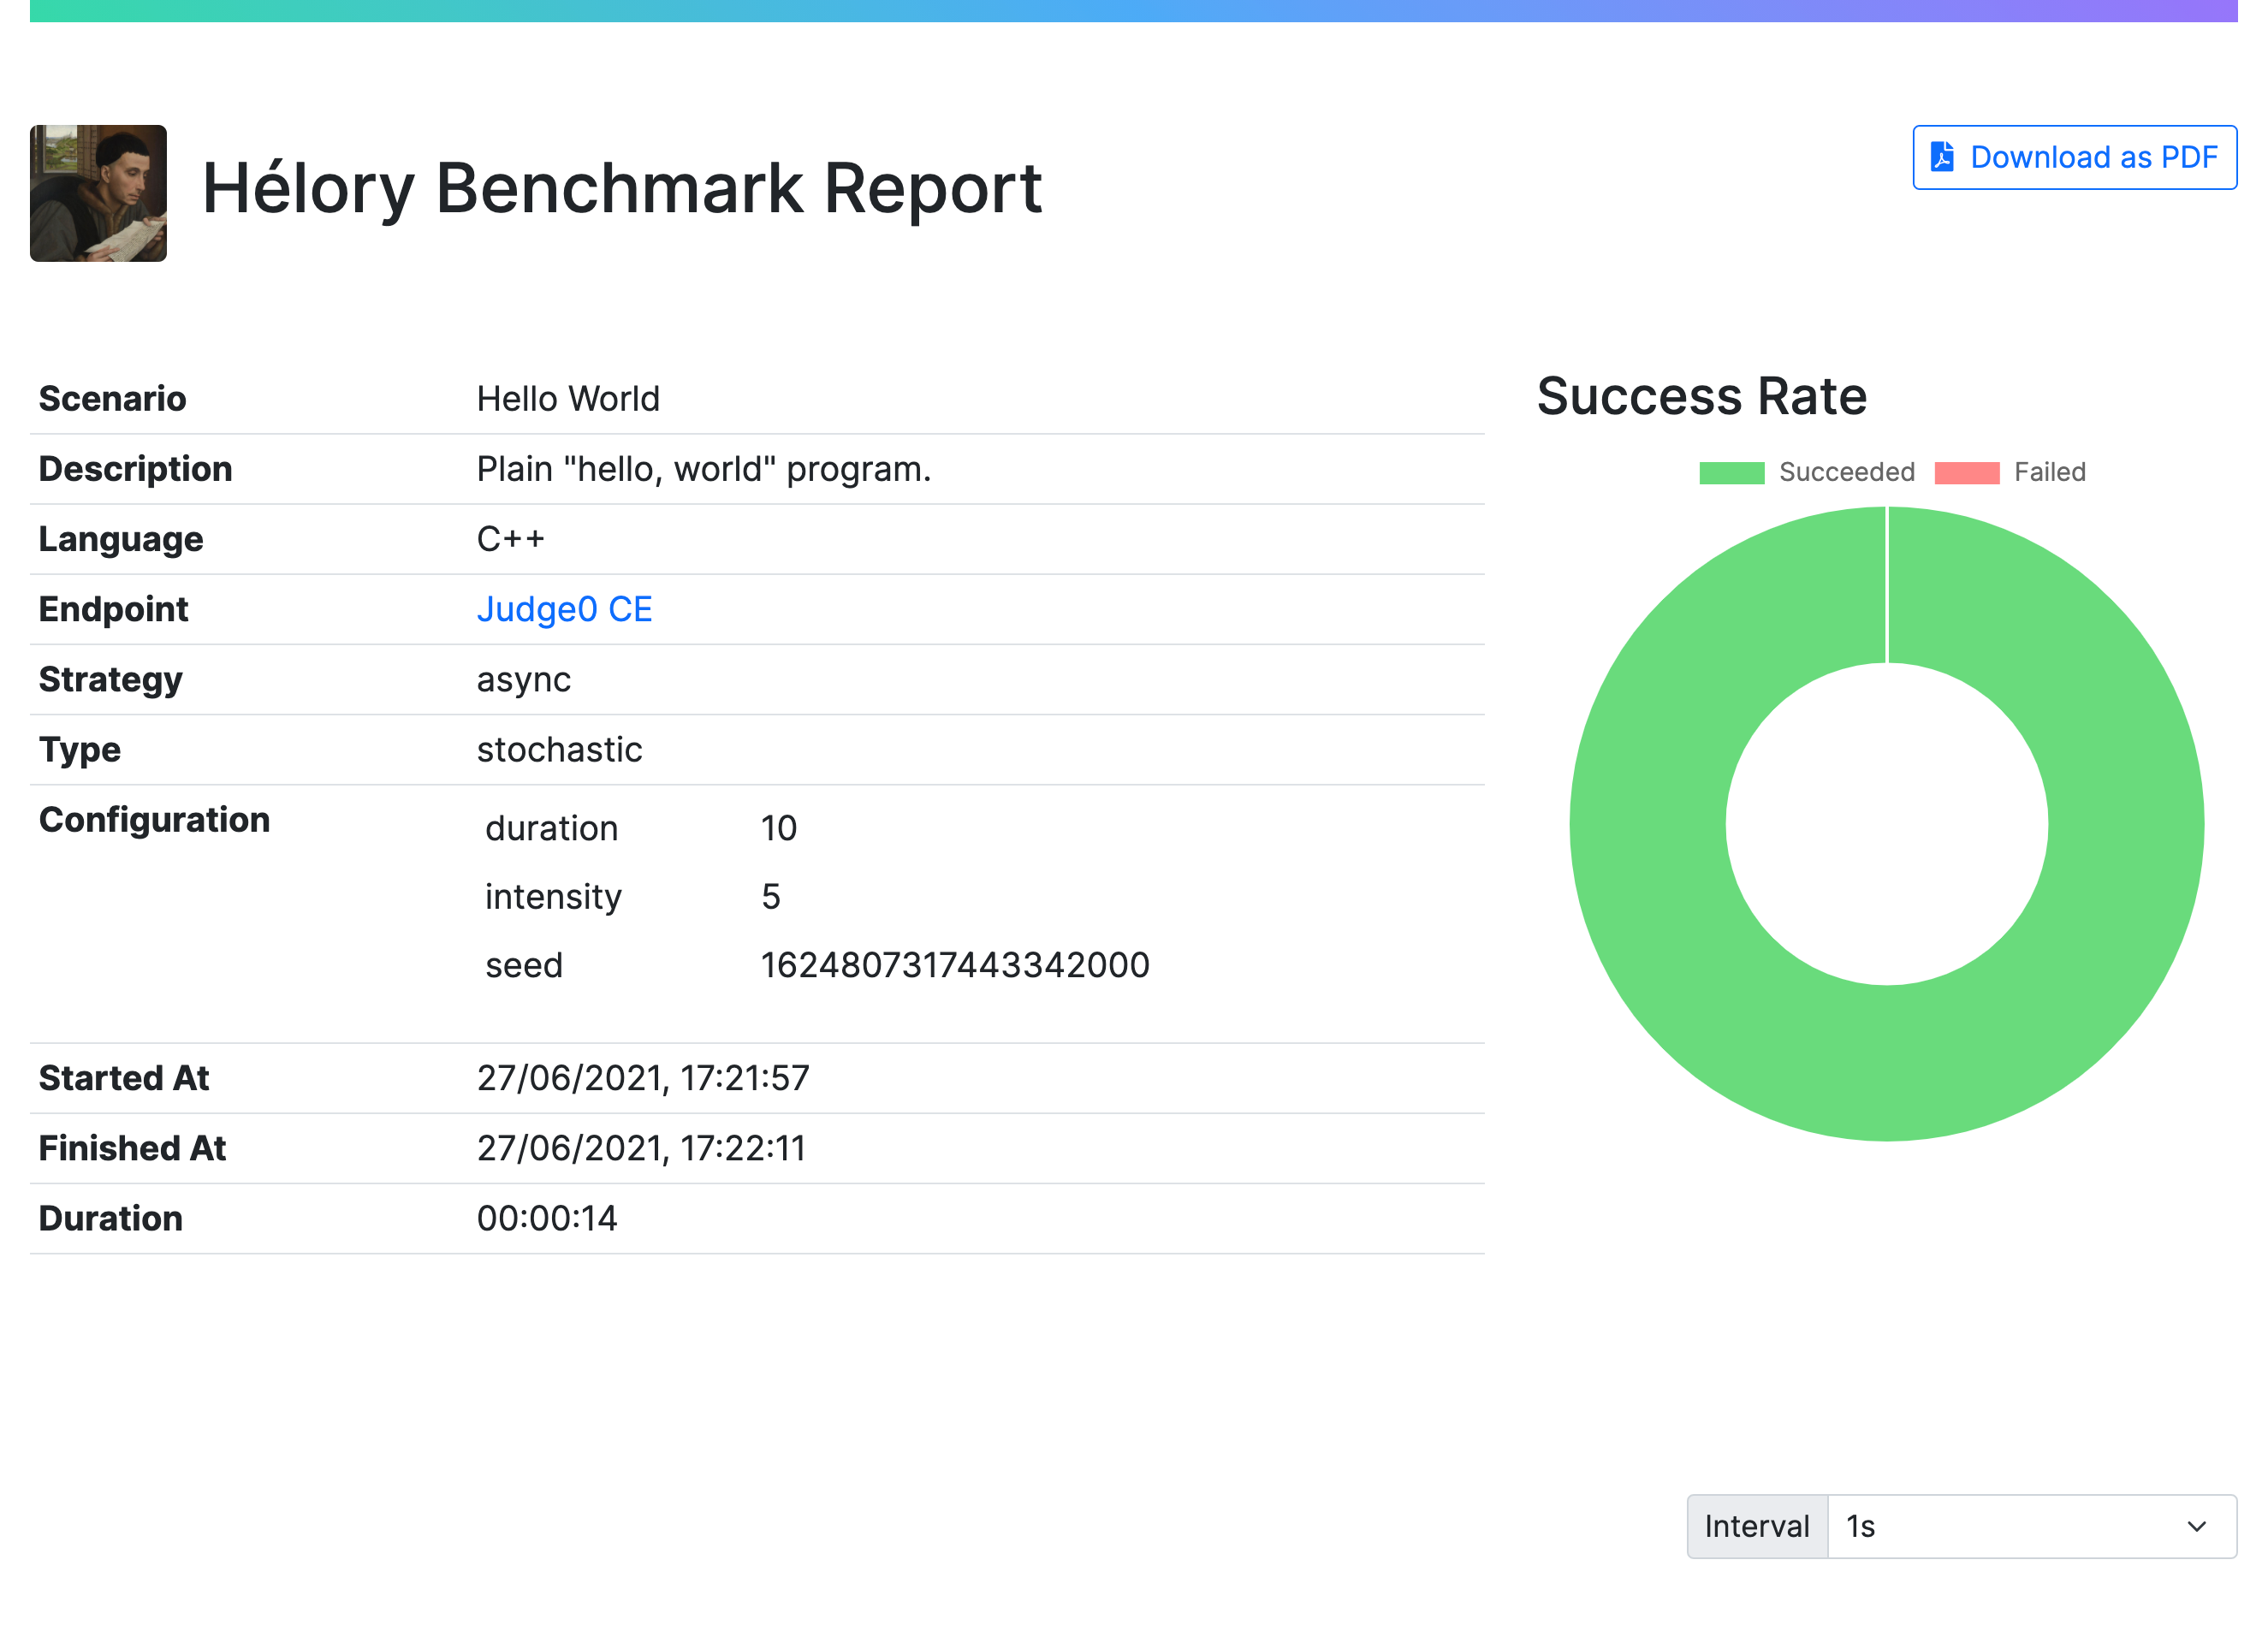
\includegraphics[width=\textwidth]{images/Report UI 1.png}
	\caption{
		Prikaz detalja o pokrenutom eksperimentu.
	}
	\label{fig:report-experiment-details}
\end{figure}

Slika \ref{fig:report-tat} prikazuje drugi dio grafičkog sučelja izvješća koji prikazuje kutijaste dijagrame \engl{box plots} vremena obrade zahtjeva grupiranih prema vremenu završetka slanja podataka u zahtjevu narudžbe koristeći odabrani korak jedinice vremena. U ovom slučaju odabrani korak jedinice vremena je 1 sekunda, što znači da će u isti kutijasti dijagram biti grupirani svi zahtjevi koji su u istoj sekundi završili slanje podataka u zahtjevu narudžbe. 

Sljedeći graf koji prikazuje izvještaj je graf prikazan na slici \ref{fig:report-requests} koji prikazuje koliko je zahtjeva u istom vremenskom trenutku odabranog koraka:
\begin{itemize}
    \item[$\bullet$] \textit{Started Orders} - započeo zahtjev narudžbe,
    \item[$\bullet$] \textit{Sent Orders} - poslao zahtjev narudžbe,
    \item[$\bullet$] \textit{Finished Orders} - završio zahtjev narudžbe,
    \item[$\bullet$] \textit{Started Probes} - započeo zahtjev ispitivanja,
    \item[$\bullet$] \textit{Finished Probes} - završio zahtjev ispitivanja, i
    \item[$\bullet$] \textit{Finished Executions} - završio zahtjev izvršavanja.
\end{itemize}

\pagebreak

\begin{figure}[htb]
	\centering
	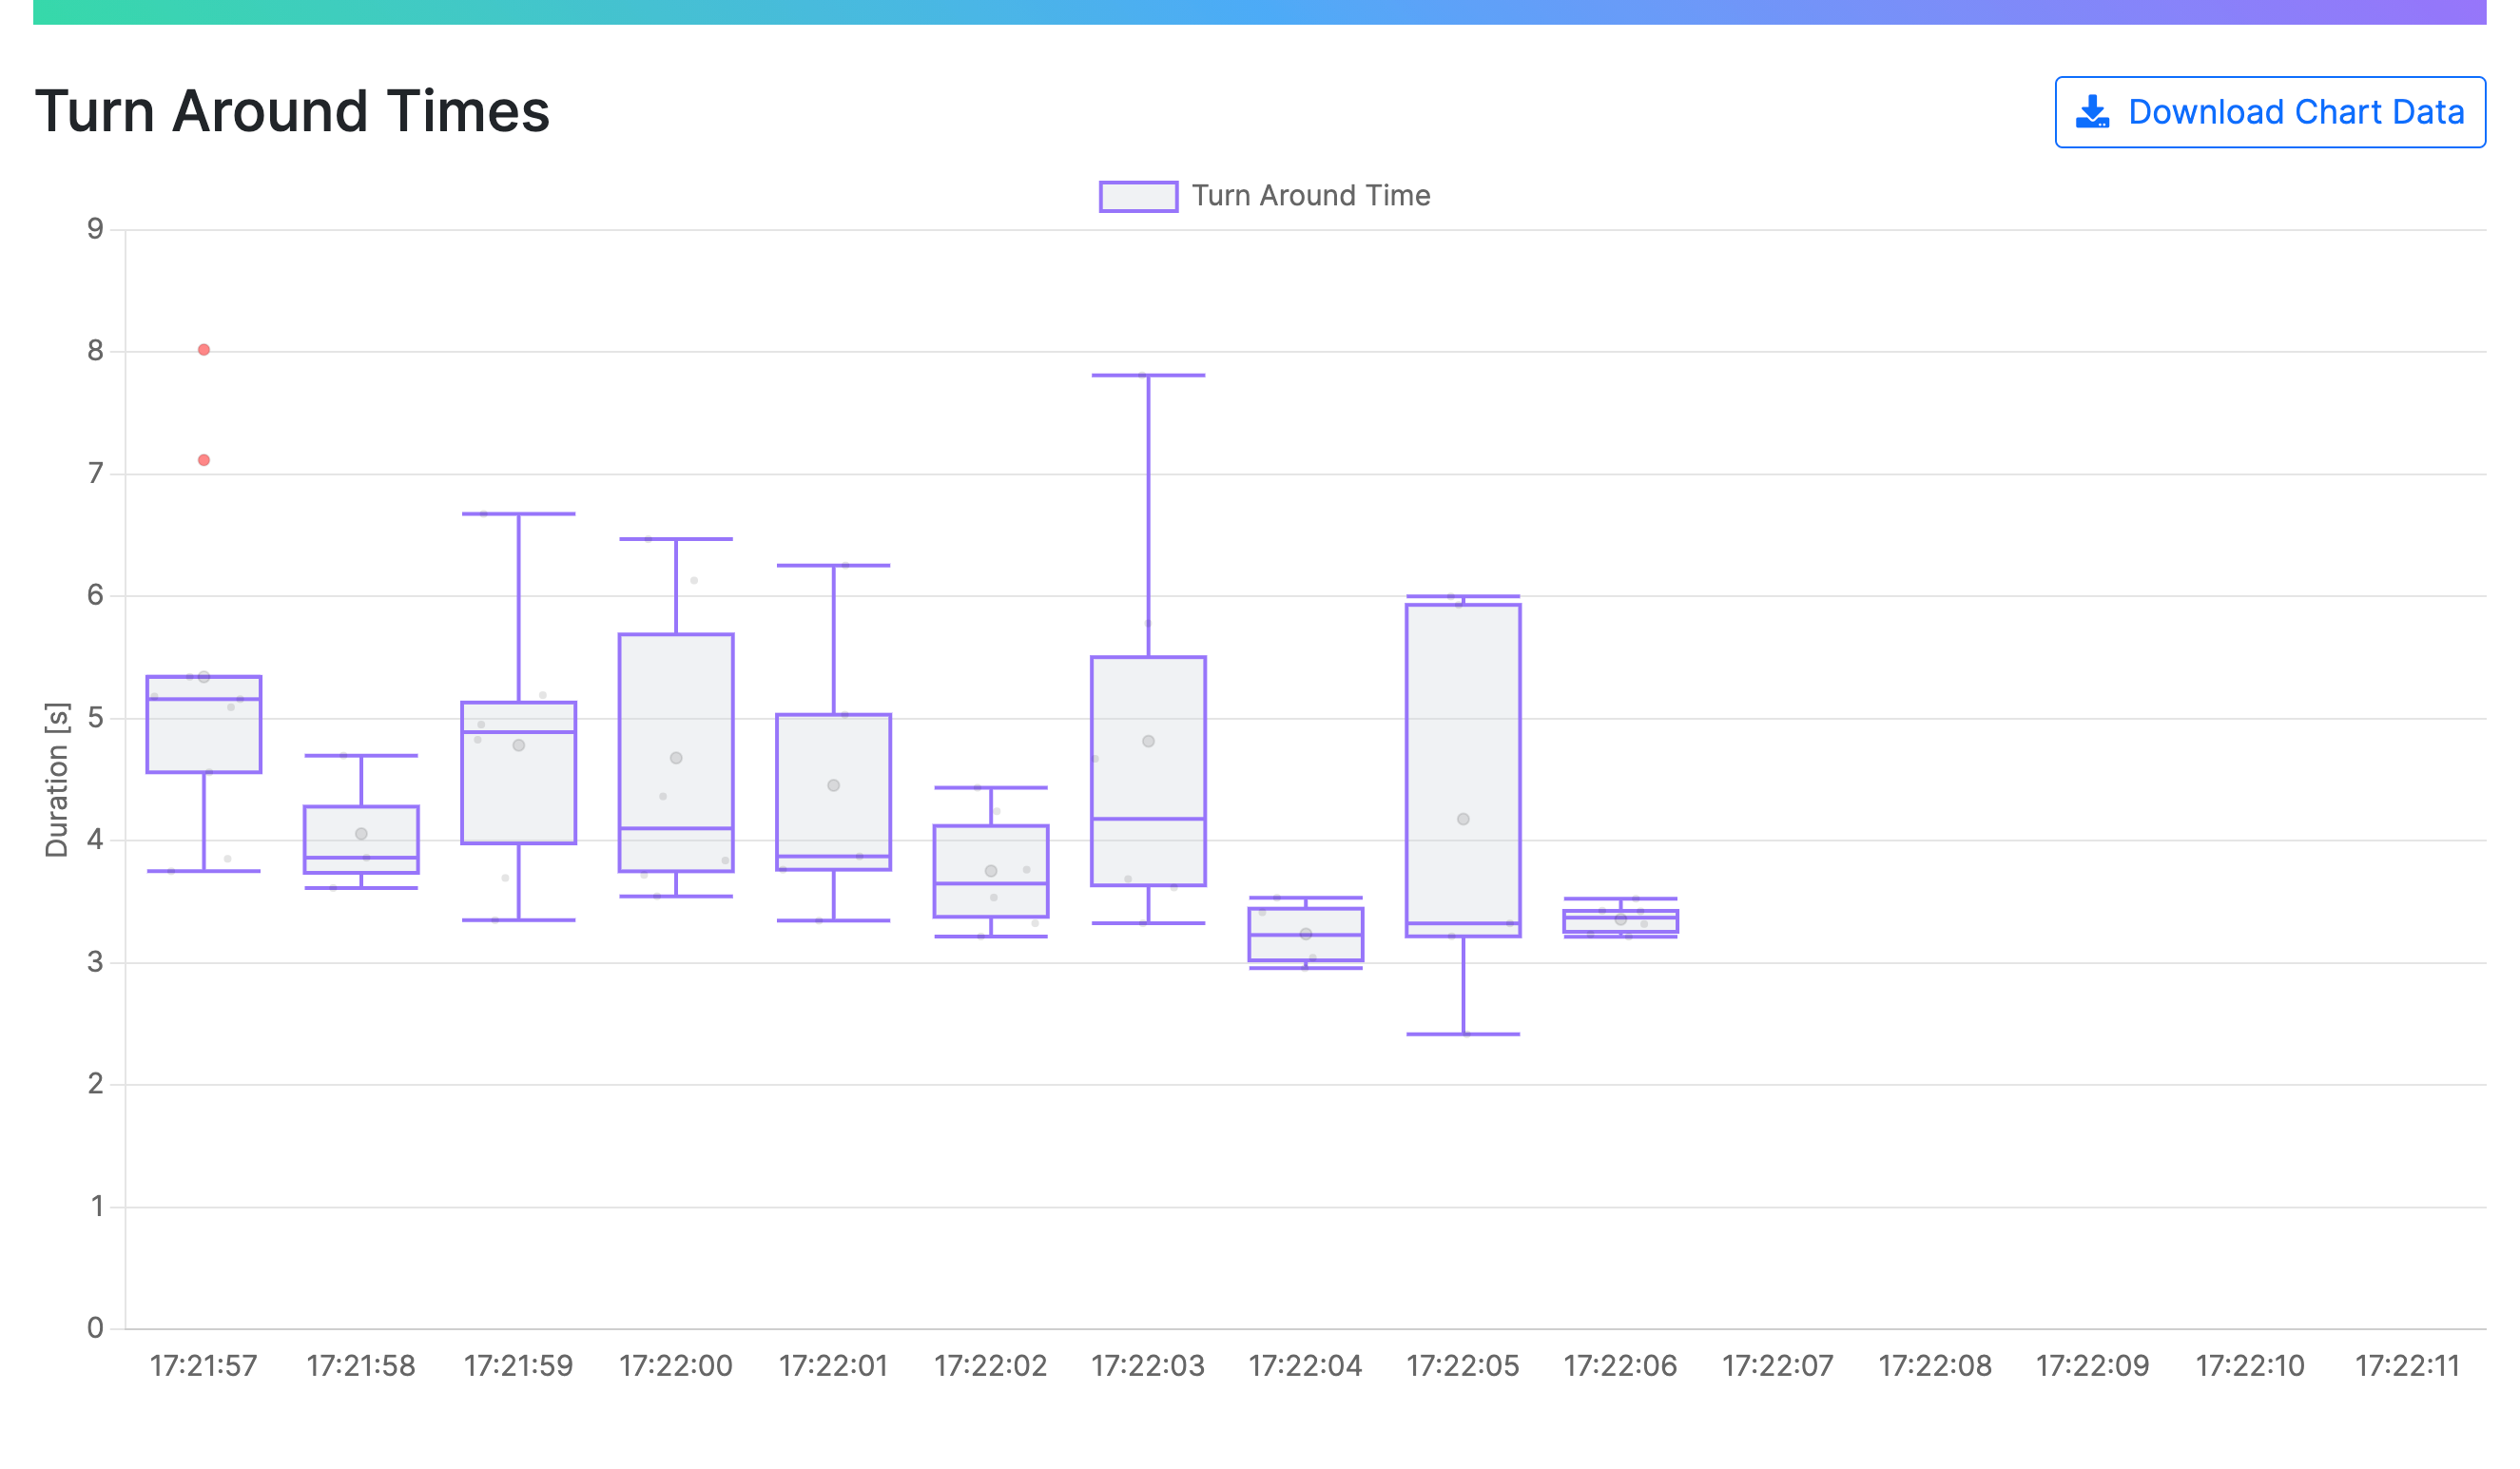
\includegraphics[width=0.91\textwidth]{images/Report UI 2.png}
	\caption{
		Prikaz dijagrama vremena obrade zahtjeva.
	}
	\label{fig:report-tat}
\end{figure}

\begin{figure}[htb]
	\centering
	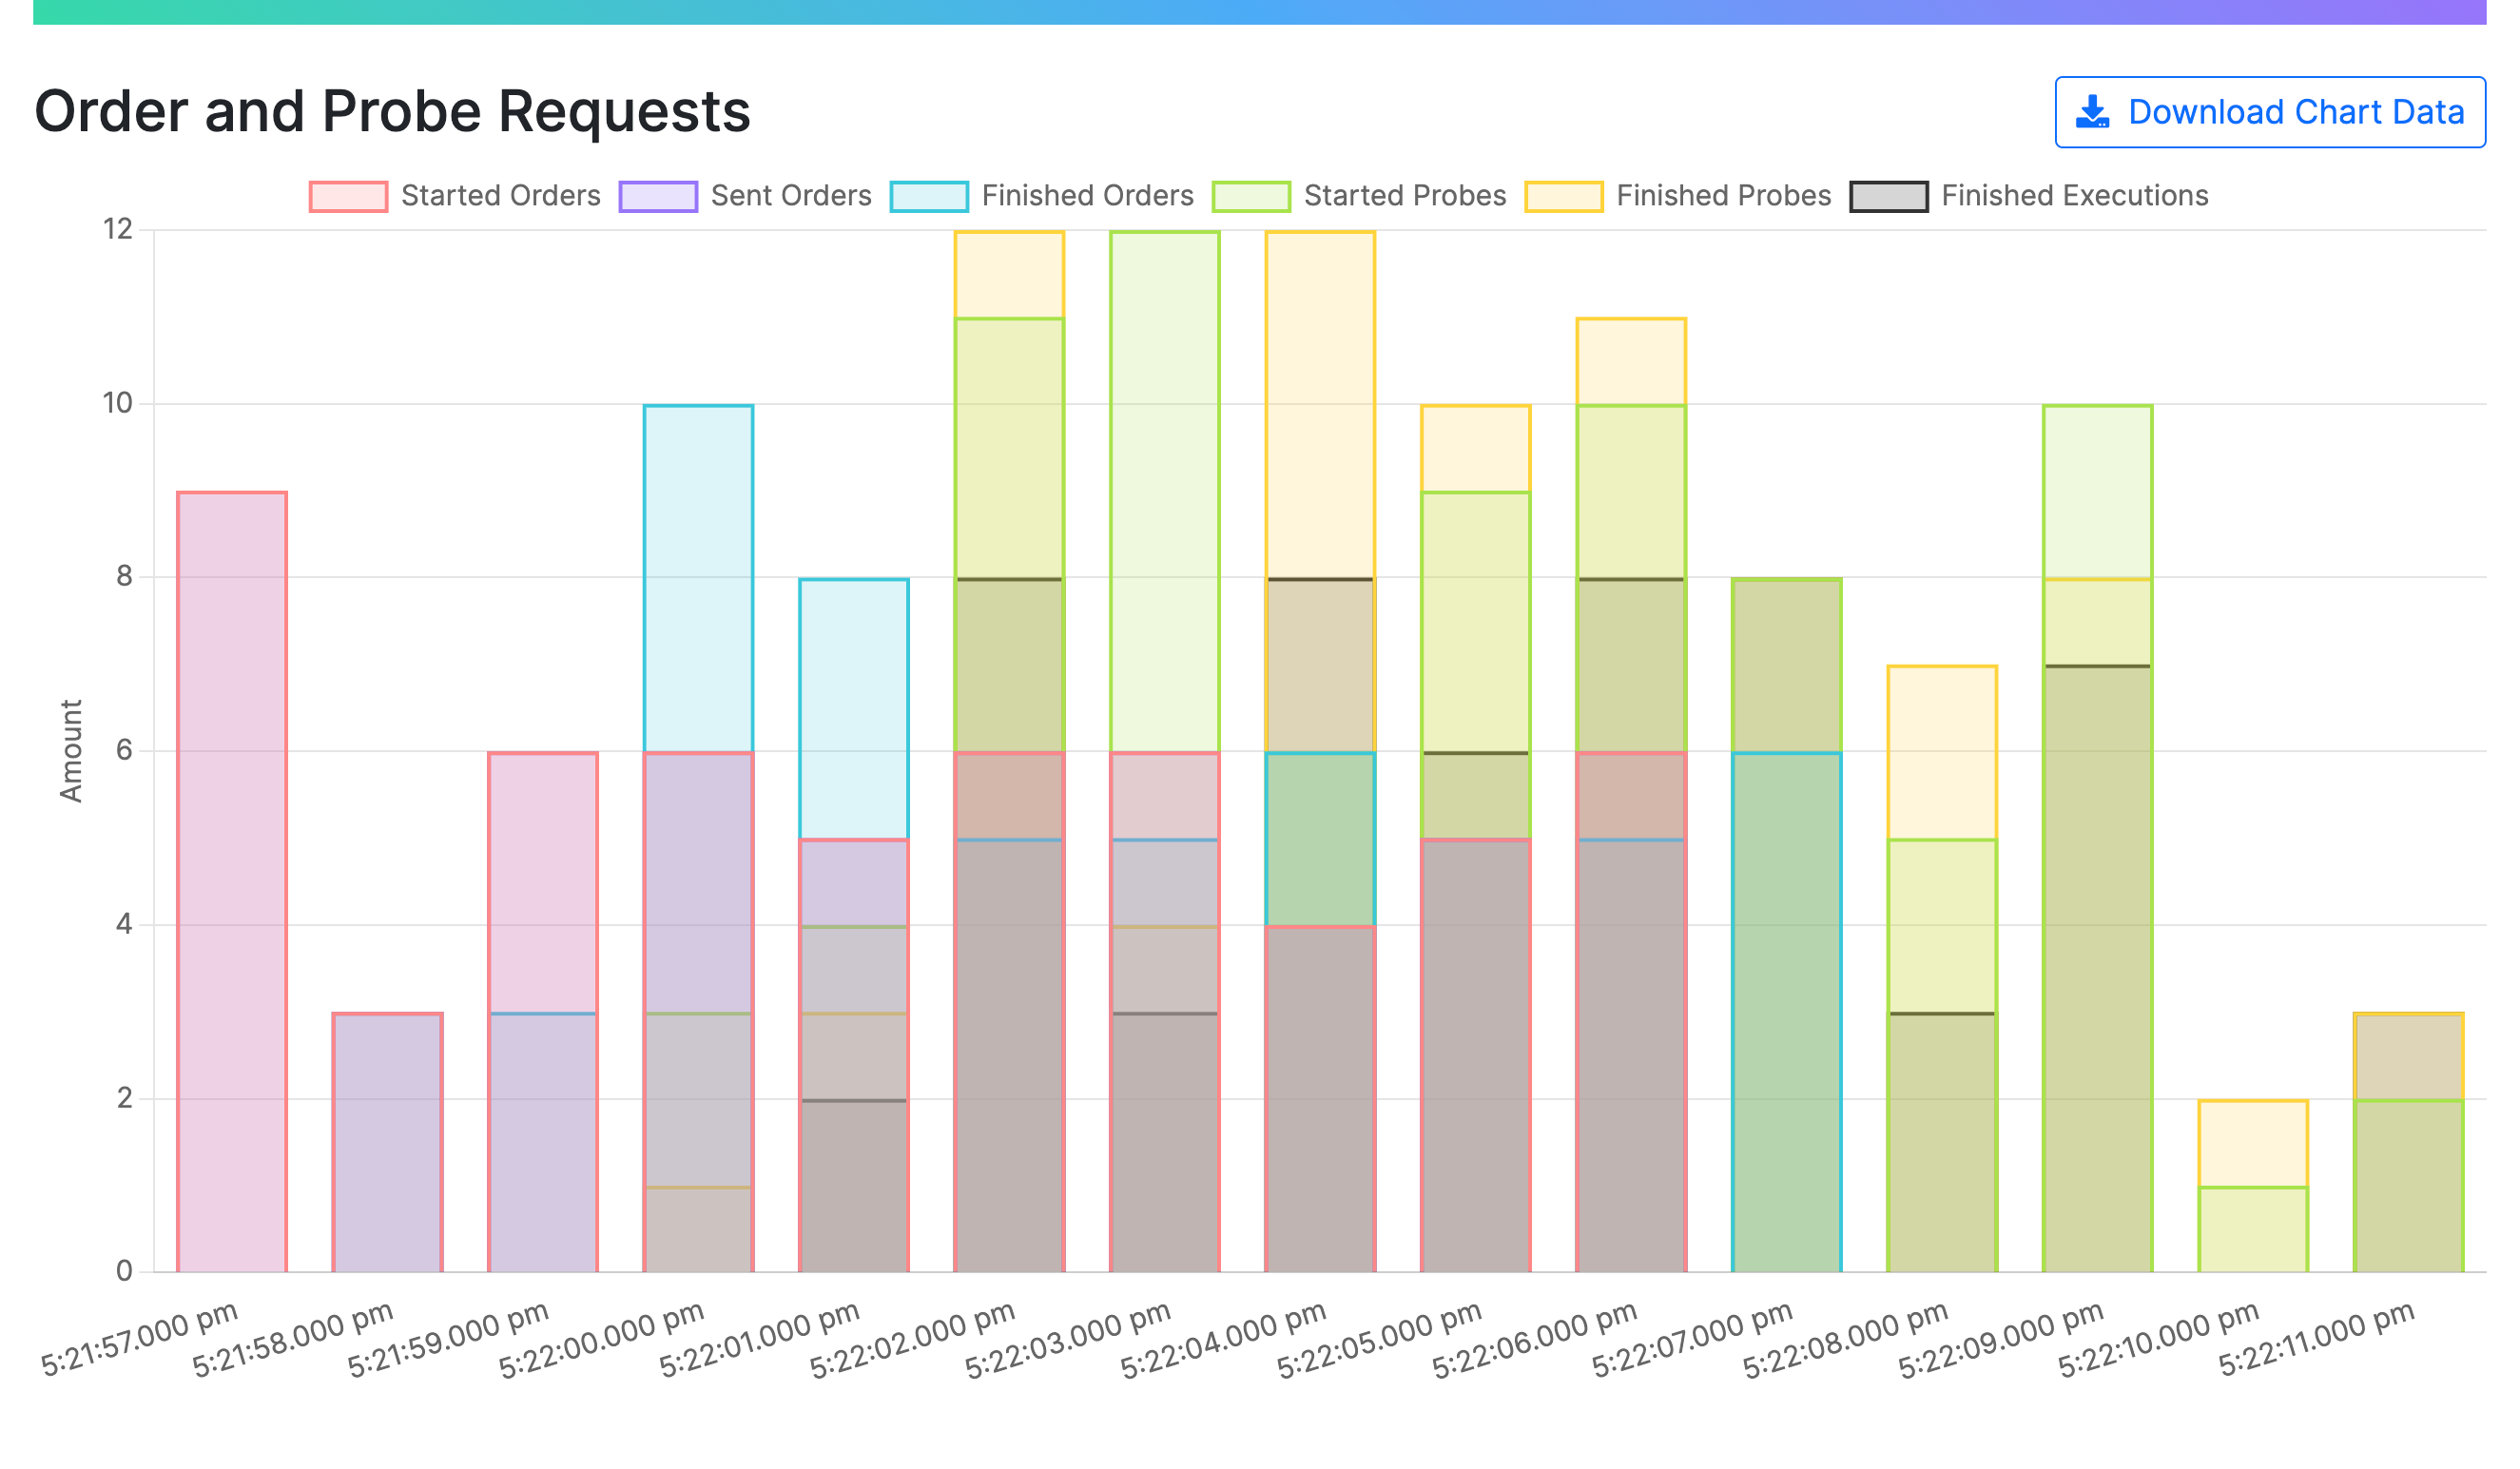
\includegraphics[width=0.91\textwidth]{images/Report UI 3.png}
	\caption{
		Prikaz grafa zahtjeva narudžbe i zahtjeva ispitivanja.
	}
	\label{fig:report-requests}
\end{figure}

\pagebreak

Konačno, slika \ref{fig:report-raw-data} prikazuje sirove podatke u formatu JSON koji su prikupljeni za vrijeme trajanja eksperimenta, a na temelju kojih su napravljeni prethnodno navedeni grafovi. Ove podatke moguće je preuzeti u formatu JSON i dodatno obraditi.

\begin{figure}[htb]
	\centering
	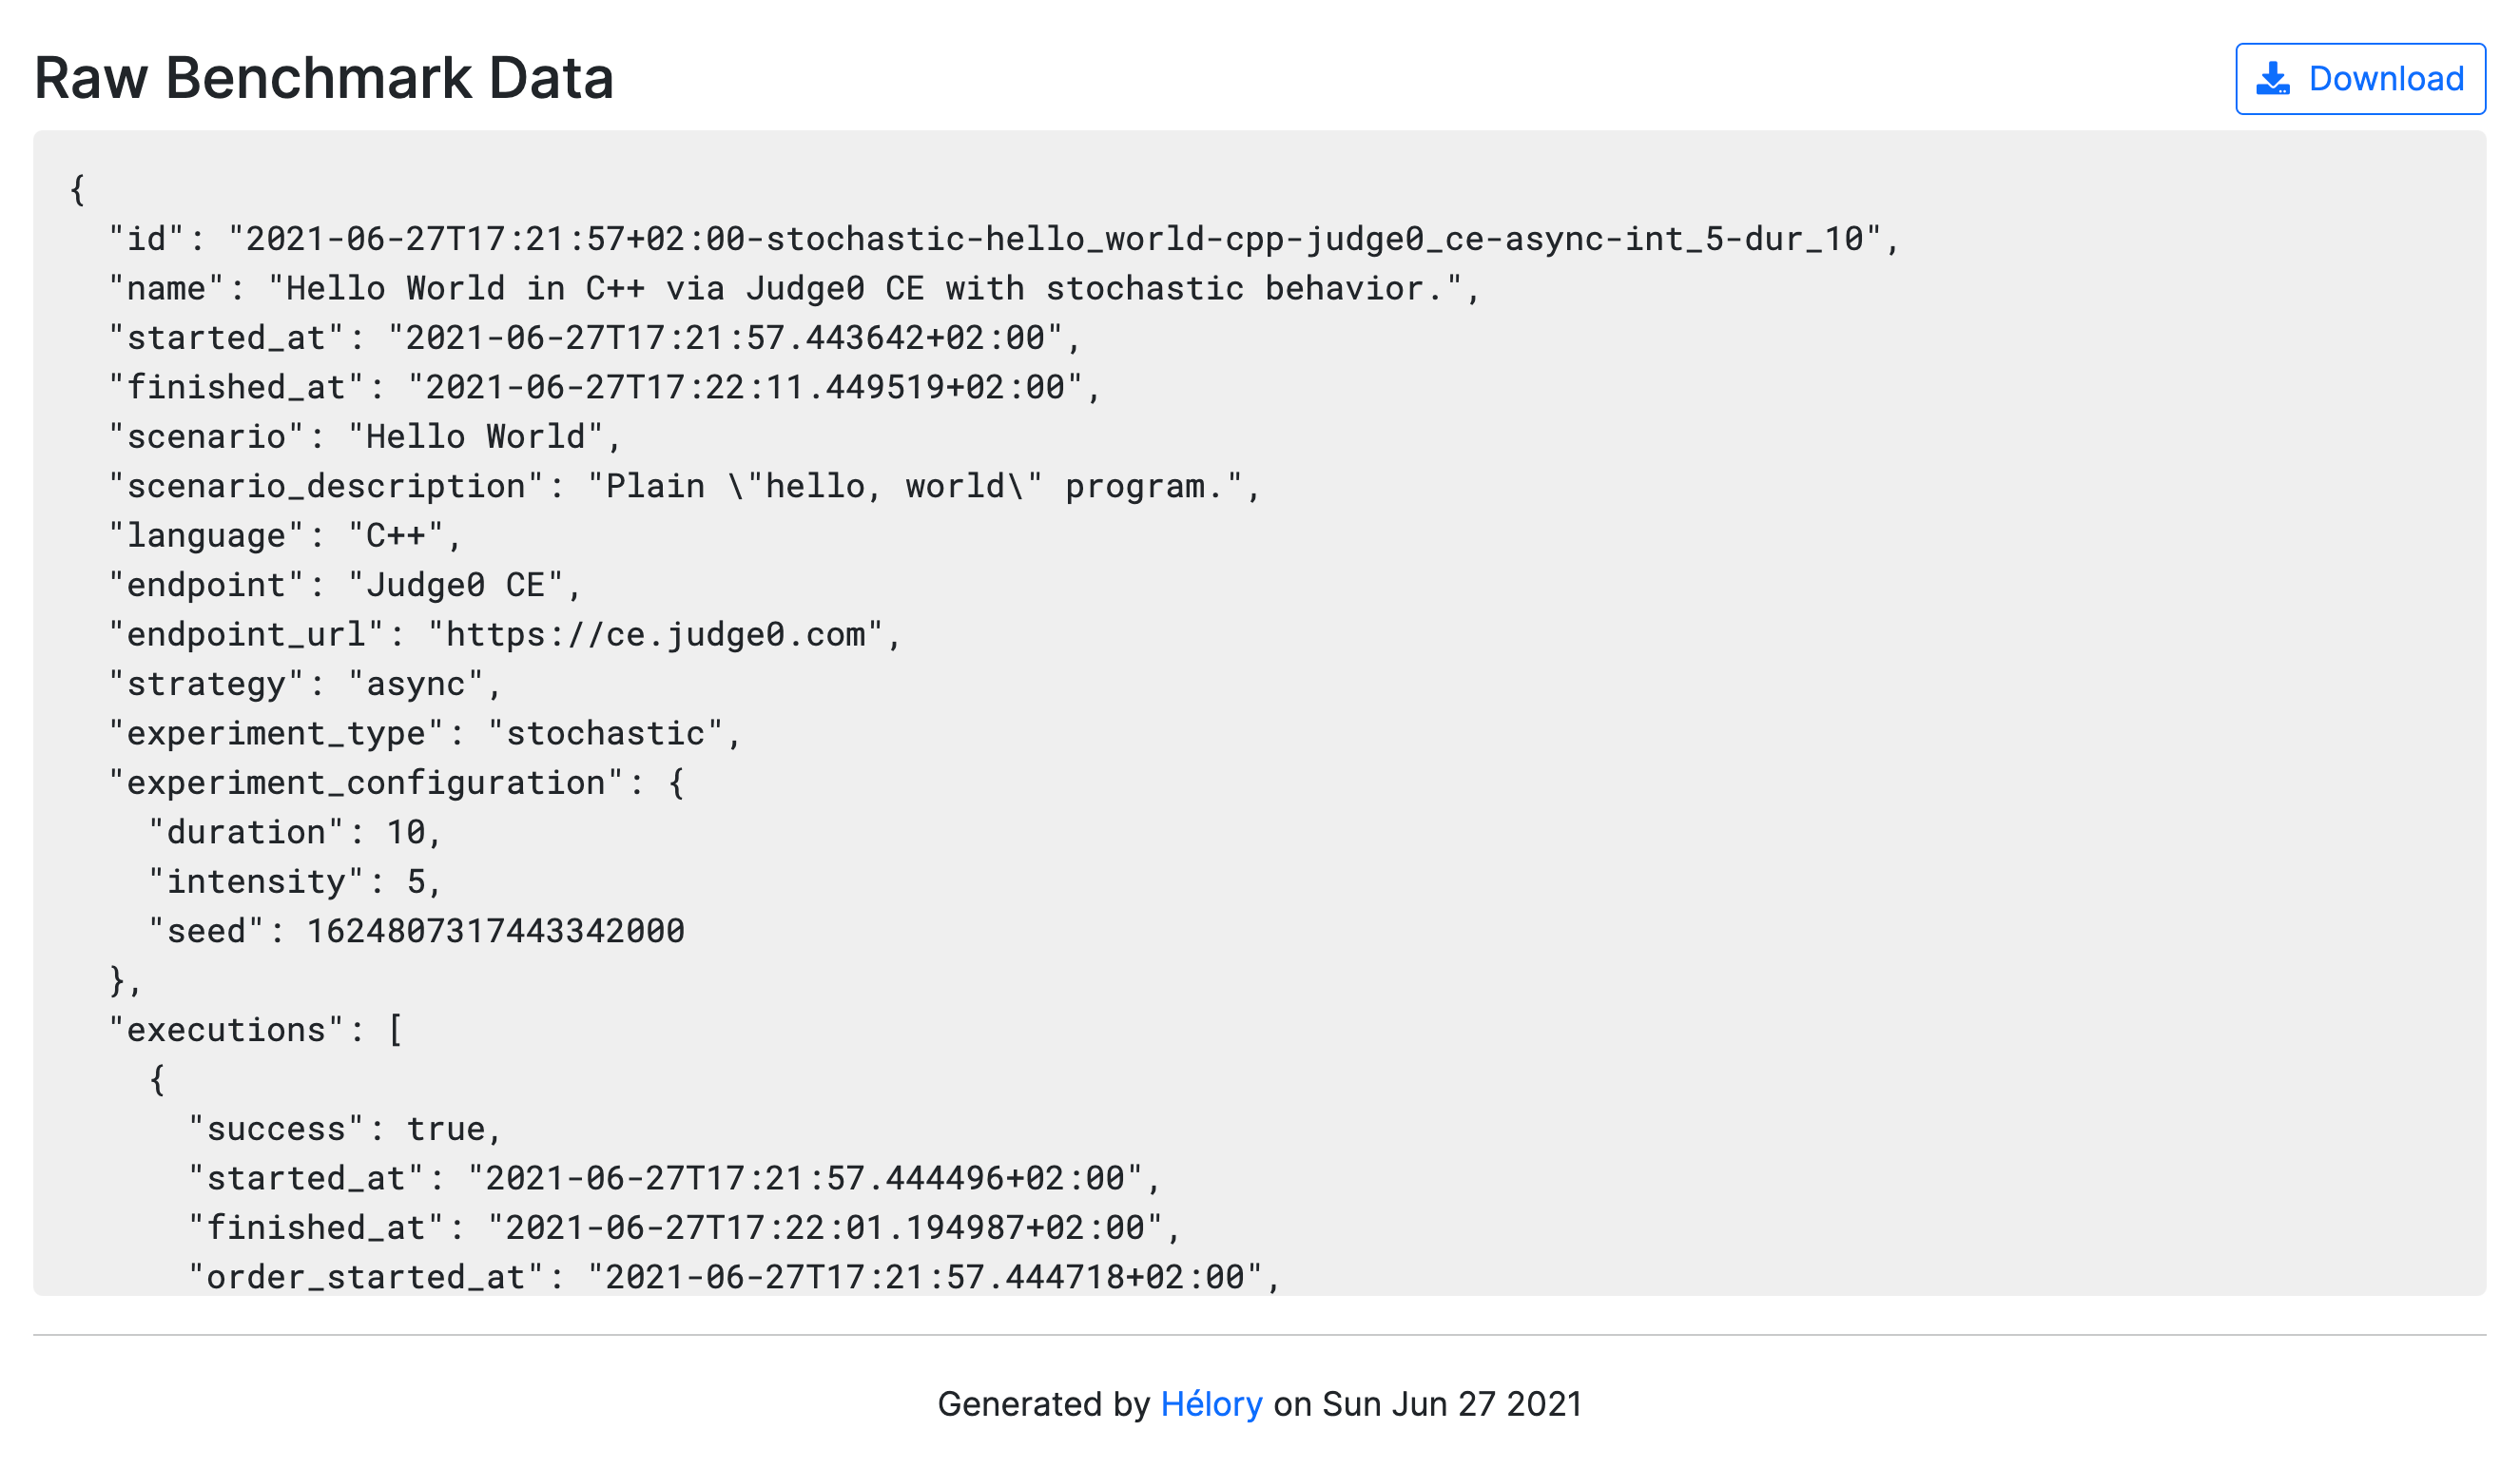
\includegraphics[width=\textwidth]{images/Report UI 4.png}
	\caption{
		Prikaz sirovih podatak prikupljenih za vrijeme eksperimenta.
	}
	\label{fig:report-raw-data}
\end{figure}

\chapter{Primjer korištenja aplikacije Hélory}
\label{chap:use}
U ovom poglavlju prikazan je primjer korištenja aplikacije Hélory u analizi performansi sustava Piston i Judge0 koji su postavljeni na dva različita poslužitelja istih resursnih kapaciteta (2 CPU-a i 8 GB radne memorije) kupljenih preko platforme Digital Ocean. Cilj eksperimenta je ocijeniti kvalitetu i pouzdanost usluge koju nude ova dva sustava, međutim, treba uzeti u obzir da kvaliteta i pouzdanost usluge također ovisi i resursima poslužitelja, ali i načinu na koji ih sustavi iskorištavaju. Također, važno je naglasiti da su sustavi na poslužitelje instalirani prema javno dostupnim uputama bez dodatnih modifikacija.

U analizi sustava promatrat će se jednostavan scenarij u \text{C++} implementaciji koristeći kontinuirano-stohastičku dinamiku s parametrima $N \in \left\{1,5,10\right\}$ i $M=60$. Budući da sustav Piston podržava isključivo sinkronu interakciju, u eksperimentima u kojima se koristi sustav Judge0 također će se koristiti sinkrona interakcija kako bi se ta dva sustava mogla pravedno usporediti.

Dodatno, na kraju je napravljena analiza performansi instance sustava Judge0 koja se koristi na Fakultetu elektrotehnike i računarstva Sveučilišta u Zagrebu.

Od nešto više od 500 eksperimentalnih rezultata, u ovom poglavlju napravljena je analiza nekoliko najznačajnijih rezultata za gore navedene instance.

\section{Analiza performansi sustava Piston}
Prvi eksperiment višekorisničkog opterećenja kontinuirano-stohastičke dinamike s parametrima $N=1$ i $M=60$ trajao je 60 sekundi i svi su zahtjevi uspješno obrađeni. Slika \ref{fig:piston-1} prikazuje vrijeme obrade zahtjeva grupiranih u intervale po 5 sekundi. Medijan vrijeme obrade svake grupe zahtjeve je između 0,5 i 1 sekunde što znači da sustav dobro podnosi opterećenje. 

Međutim, prilikom povećanja opterećenja na $N=5$ udio uspješno obrađenih zahtjeva pada na 82,98\%, a medijan vrijeme obrade zahtjeva raste i do 55 sekundi (slika \ref{fig:piston-2}). Sustav Piston još teže podnosi opterećenje za $N=10$ kada udio uspješno obrađenih zahtjeva dodatno padne na 42,44\%.

Dodatno provedeni eksperimenti pokazuju da sustav Piston ne obradi uspješno niti jedan zahtjev za opterećenje $N=1$ scenarija procesorskog opterećenja u \text{C++} implementaciji.

Daljnja analiza performansi sustava Piston nije potrebna budući da za jednostavan scenarij korištenja ne prikazuje dobre rezultate niti po pitanju performansi, niti pouzdanosti, a rezultati pokazuju da sustav Piston podnosi srednje opterećenje od jednog zahtjeva u sekundi jednostavnog scenarija korištenja u C++ implementaciji.

\begin{figure}[htb]
	\centering
	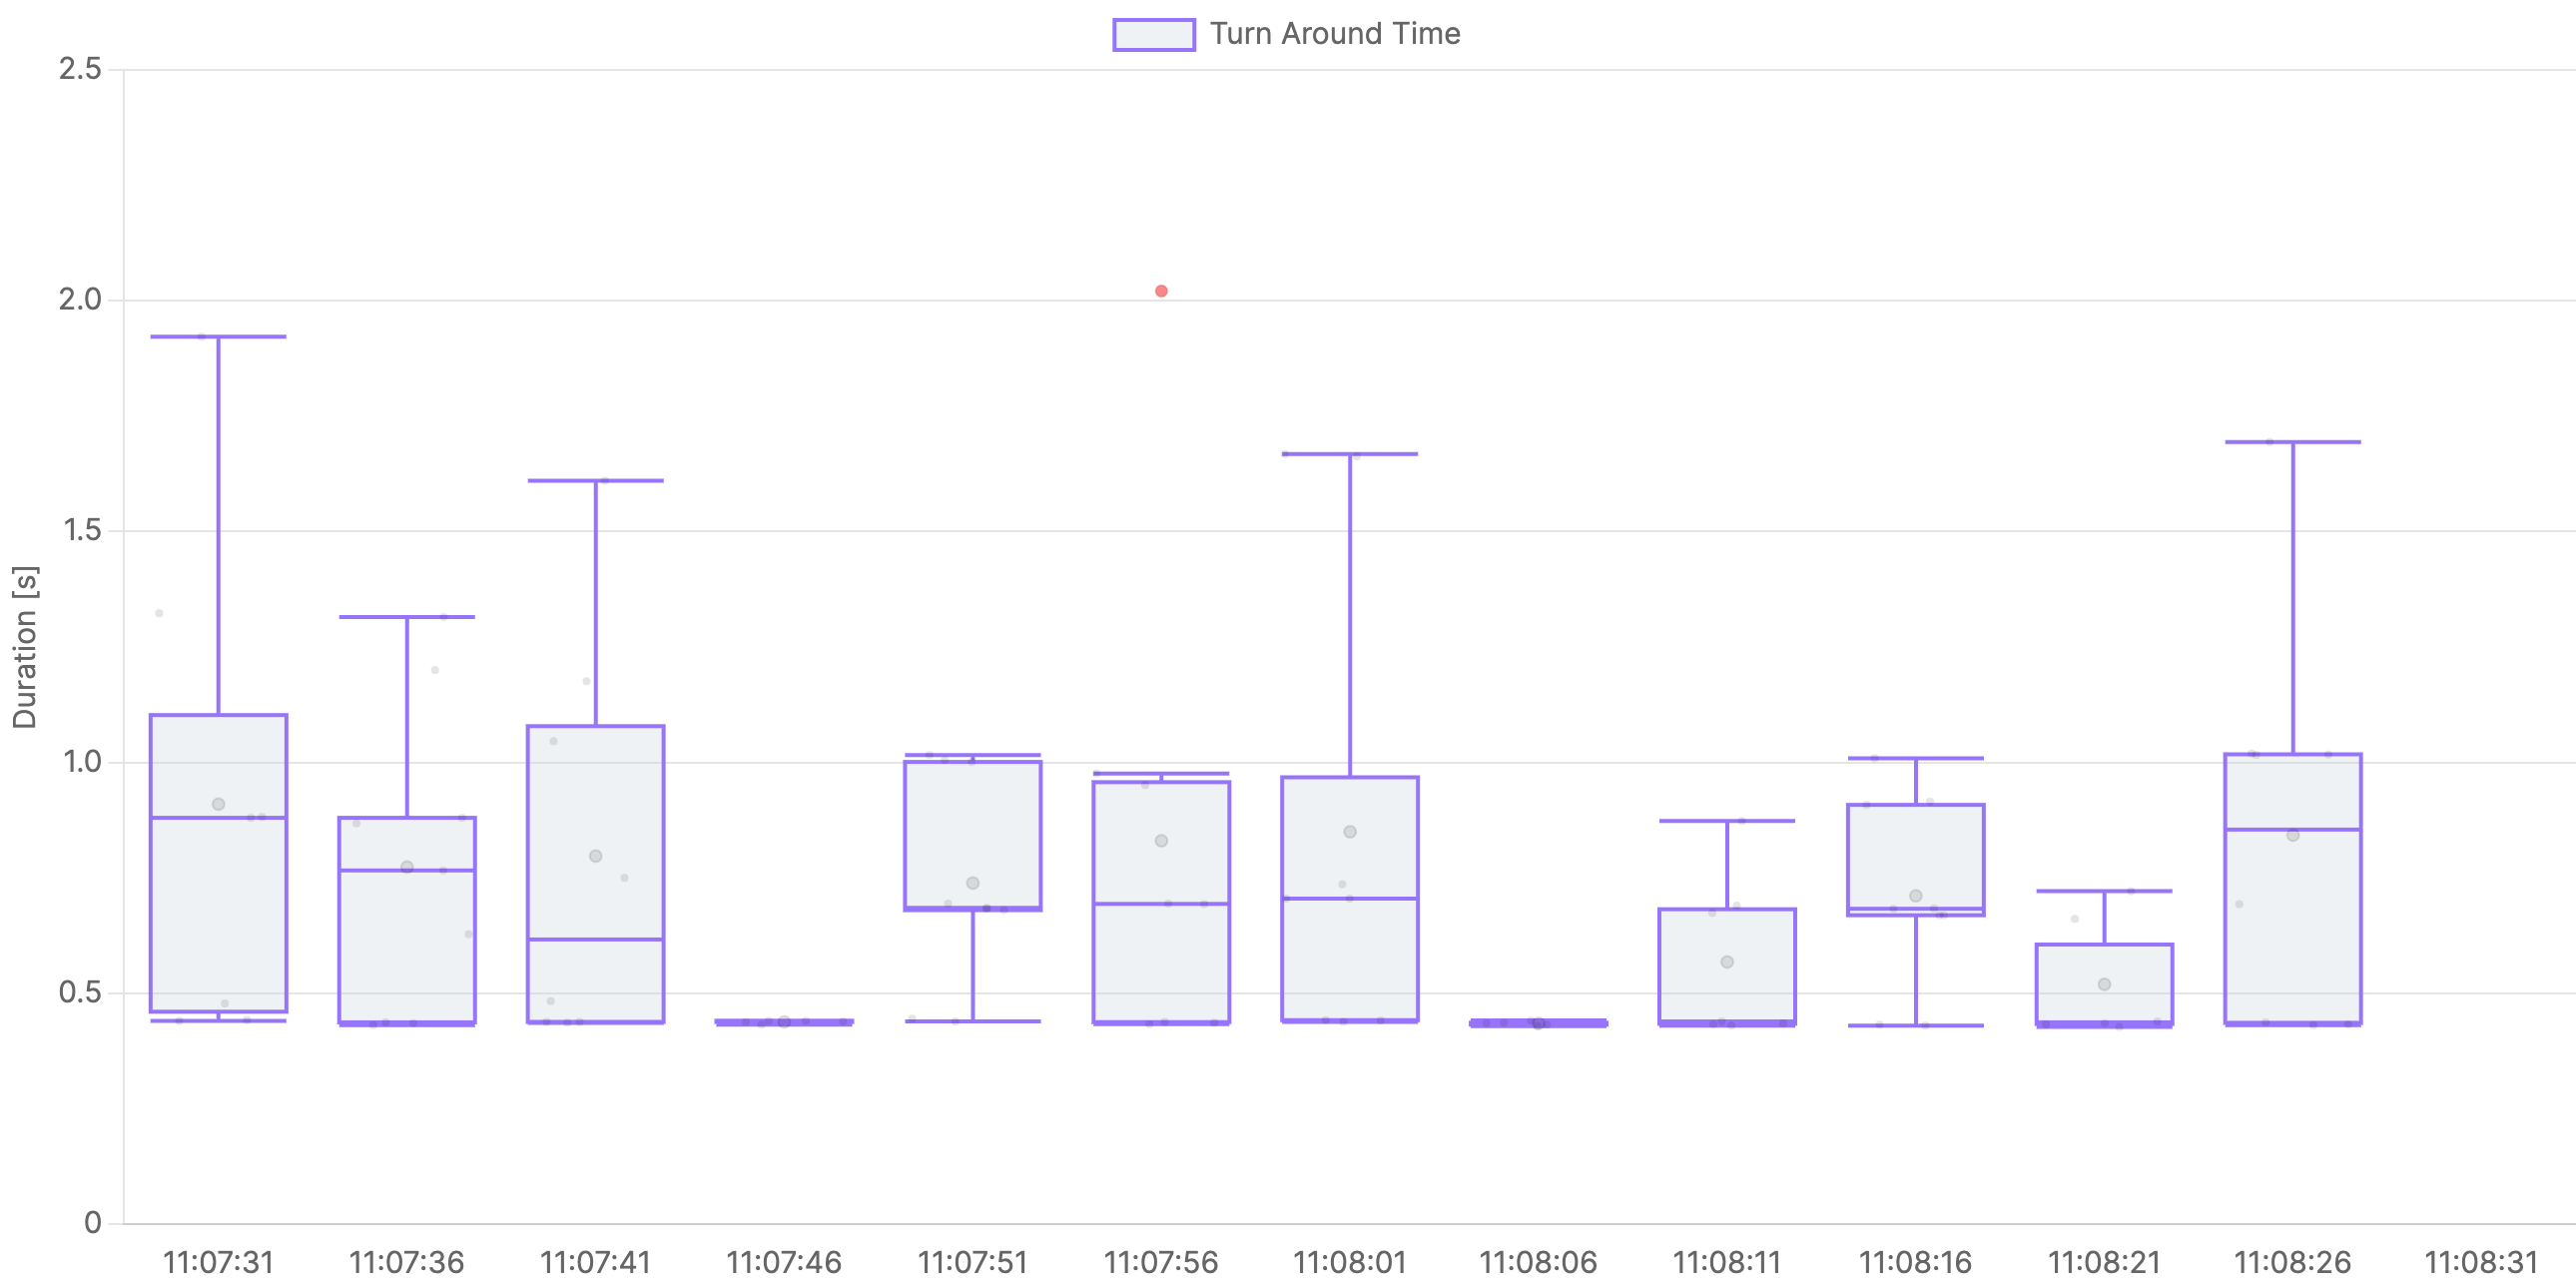
\includegraphics[width=\textwidth]{images/Piston TAT for 1 5s.png}
	\caption{
		Vrijeme obrade zahtjeva sustava Piston za $N=1$ i $M=60$.
	}
	\label{fig:piston-1}
\end{figure}

\begin{figure}[htb]
	\centering
	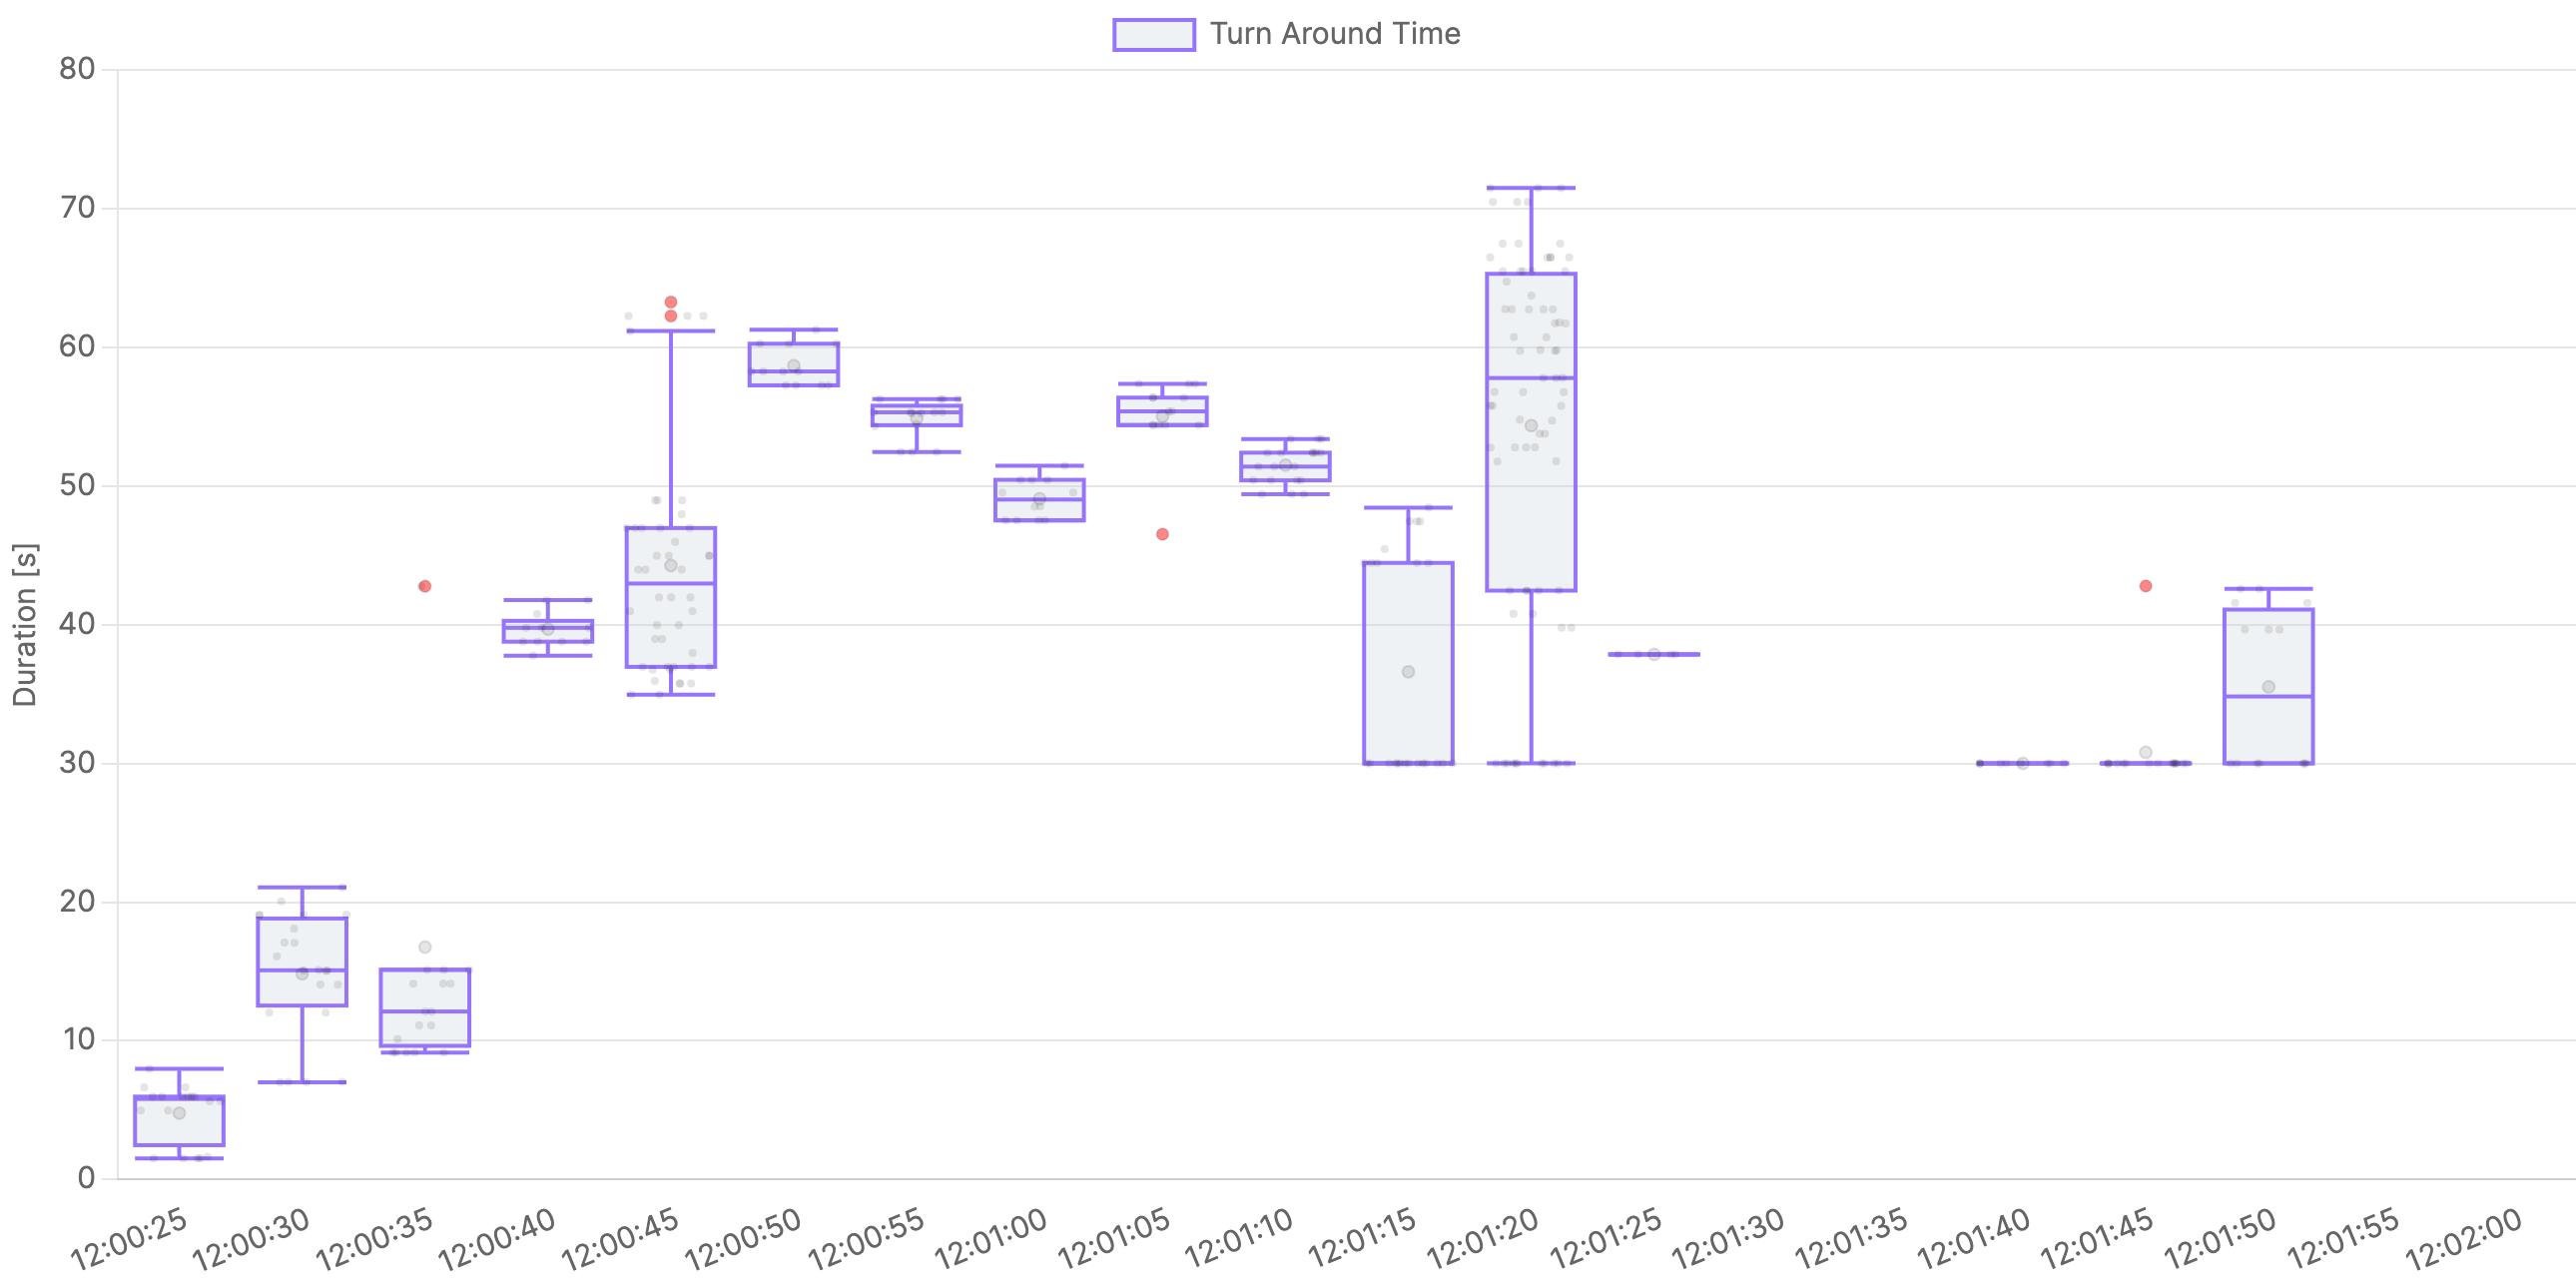
\includegraphics[width=\textwidth]{images/Piston TAT for 5 5s.png}
	\caption{
		Vrijeme obrade zahtjeva sustava Piston za $N=5$ i $M=60$.
	}
	\label{fig:piston-2}
\end{figure}

\pagebreak

\section{Analiza performansi sustava Judge0}
Sustavu Judge0 pri opterećenju $N=1$ treba 63 sekunde da uspješno obradi sve zahtjeve, međutim, medijan vrijeme obrade zahtjeva kreće se između 2 i 5 sekundi (slika \ref{fig:judge0-1}) što je nepovoljnije u odnosu na sustav Piston. 

Pri opterećenju $N=5$ Judge0 zadržava udio uspješno obrađenih zahtjeva, međutim, medijan vrijeme obrade zahtjeva linearno raste s vremenom trajanja eksperimenta kako prikazuje slika \ref{fig:judge0-2}.

Daljnjim povećanjem opterećenja na $N=10$ udio uspješno obrađenih zahtjeva pada na 81,79\%, a medijan vrijeme obrade zahtjeva i dalje linearno raste. Međutim, dodatnim eksperimentima utvrđeno je da pri asinkronoj interakciji istog opterećenja udio uspješno obrađenih zahtjeva 100\%, ali medijan vrijeme obrade zahtjeva opet linearno raste.

Na poslužitelju s istim resursnim kapacitetima, sustav Judge0 pokazuje bolju pouzdanost od sustava Piston uz uvjet da se koristi preporučena asinkrona interakcija, međutim, kao i sustav Piston, sustav Judge0 podnosi srednje opterećenje od jednog zahtjeva u sekundi jednostavnog scenarija korištenja u C++ implementaciji. 

\begin{figure}[htb]
	\centering
	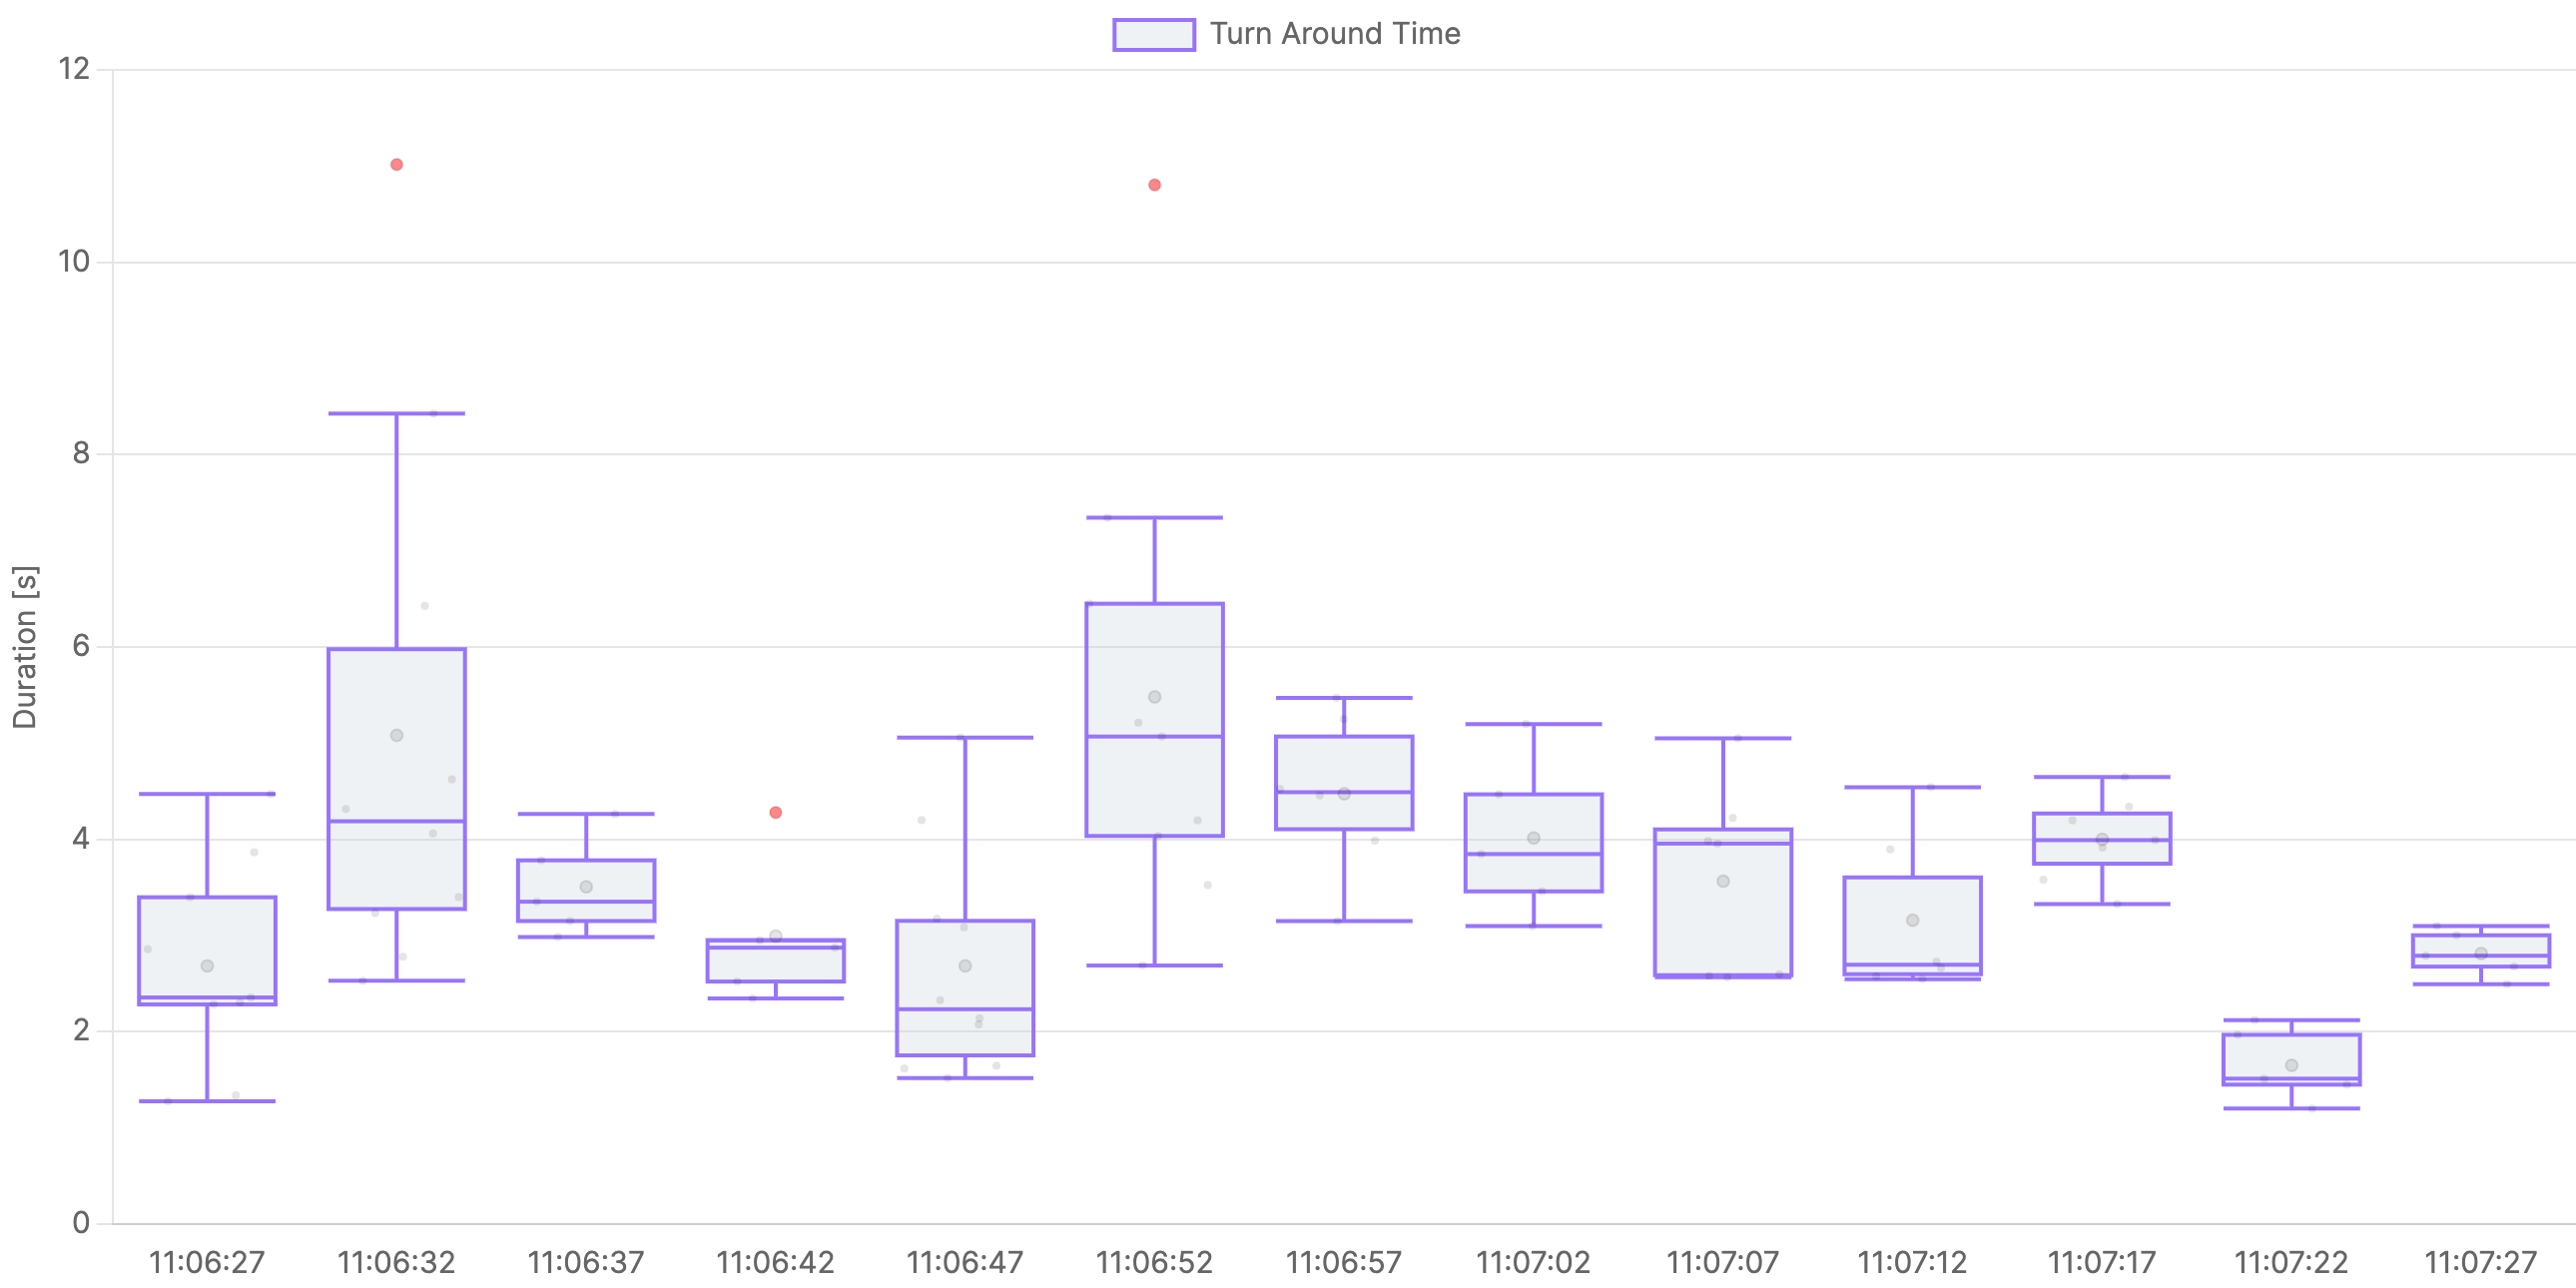
\includegraphics[width=\textwidth]{images/Judge0 TAT for 1 5s.png}
	\caption{
		Vrijeme obrade zahtjeva sustava Judge0 za $N=1$ i $M=60$.
	}
	\label{fig:judge0-1}
\end{figure}

\pagebreak

\begin{figure}[htb]
	\centering
	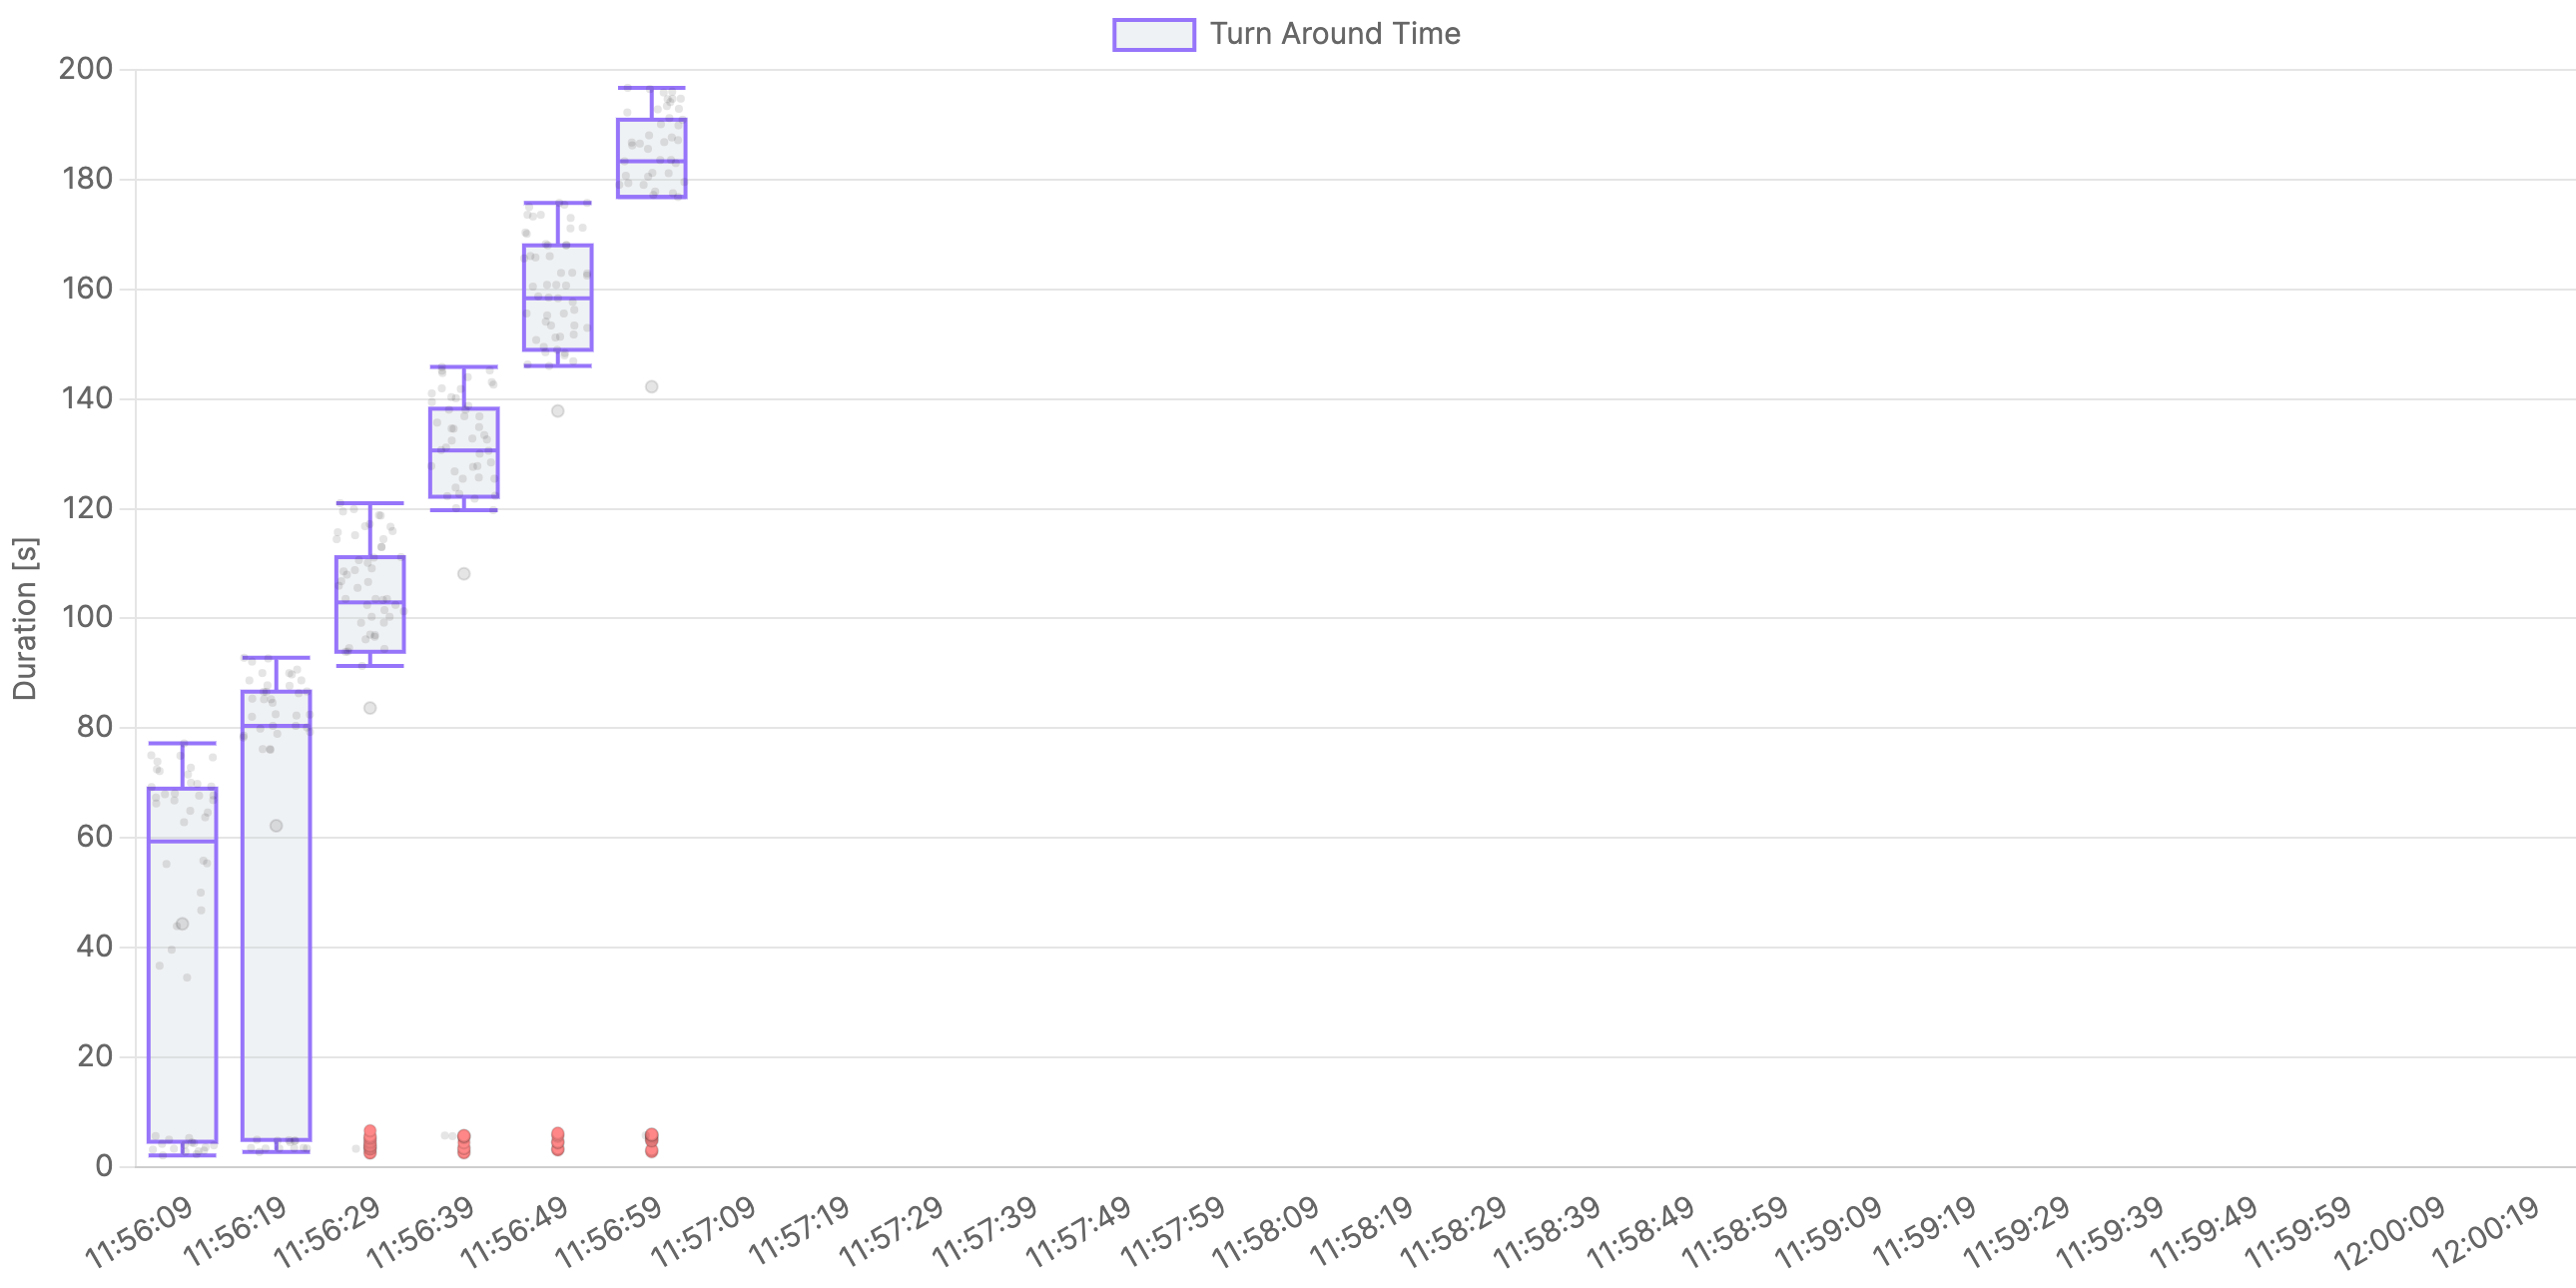
\includegraphics[width=\textwidth]{images/Judge0 TAT for 5 10s.png}
	\caption{
		Vrijeme obrade zahtjeva sustava Judge0 za $N=5$ i $M=60$.
	}
	\label{fig:judge0-2}
\end{figure}

\pagebreak

\subsubsection{Analiza performansi FER-ove instance sustava Judge0}

Instanca sustava Judge0 koja se koristi na Fakultet elektrotehnike i računarstva Sveučilišta u Zagrebu pokazuje zavidno stabilno medijan vrijeme obrade zahtjeva za kontinuirano-stohastičko opterećenje parametara $N=5$ i $M=60$ s asinkronom interakcijom za jednostavan scenarij korištenja u \text{C++} implementaciji. Slika \ref{fig:judge0-fer-1} prikazuje vrijeme obrade zahtjeva grupiranih u intervale duljine 5 sekundi. Svi zahtjevi uspješno su obrađeni. Povećanjem intenziteta na $N=20$ sustav zadržava stabilno medijan vrijeme obrade kao i u prethodnom slučaju, međutim, pri intenzitetu od $N=25$ medijan vrijeme obrade počinje rasti s vremenom trajanja eksperimenta (slika \ref{fig:judge0-fer-2}).

\begin{figure}[htb]
	\centering
	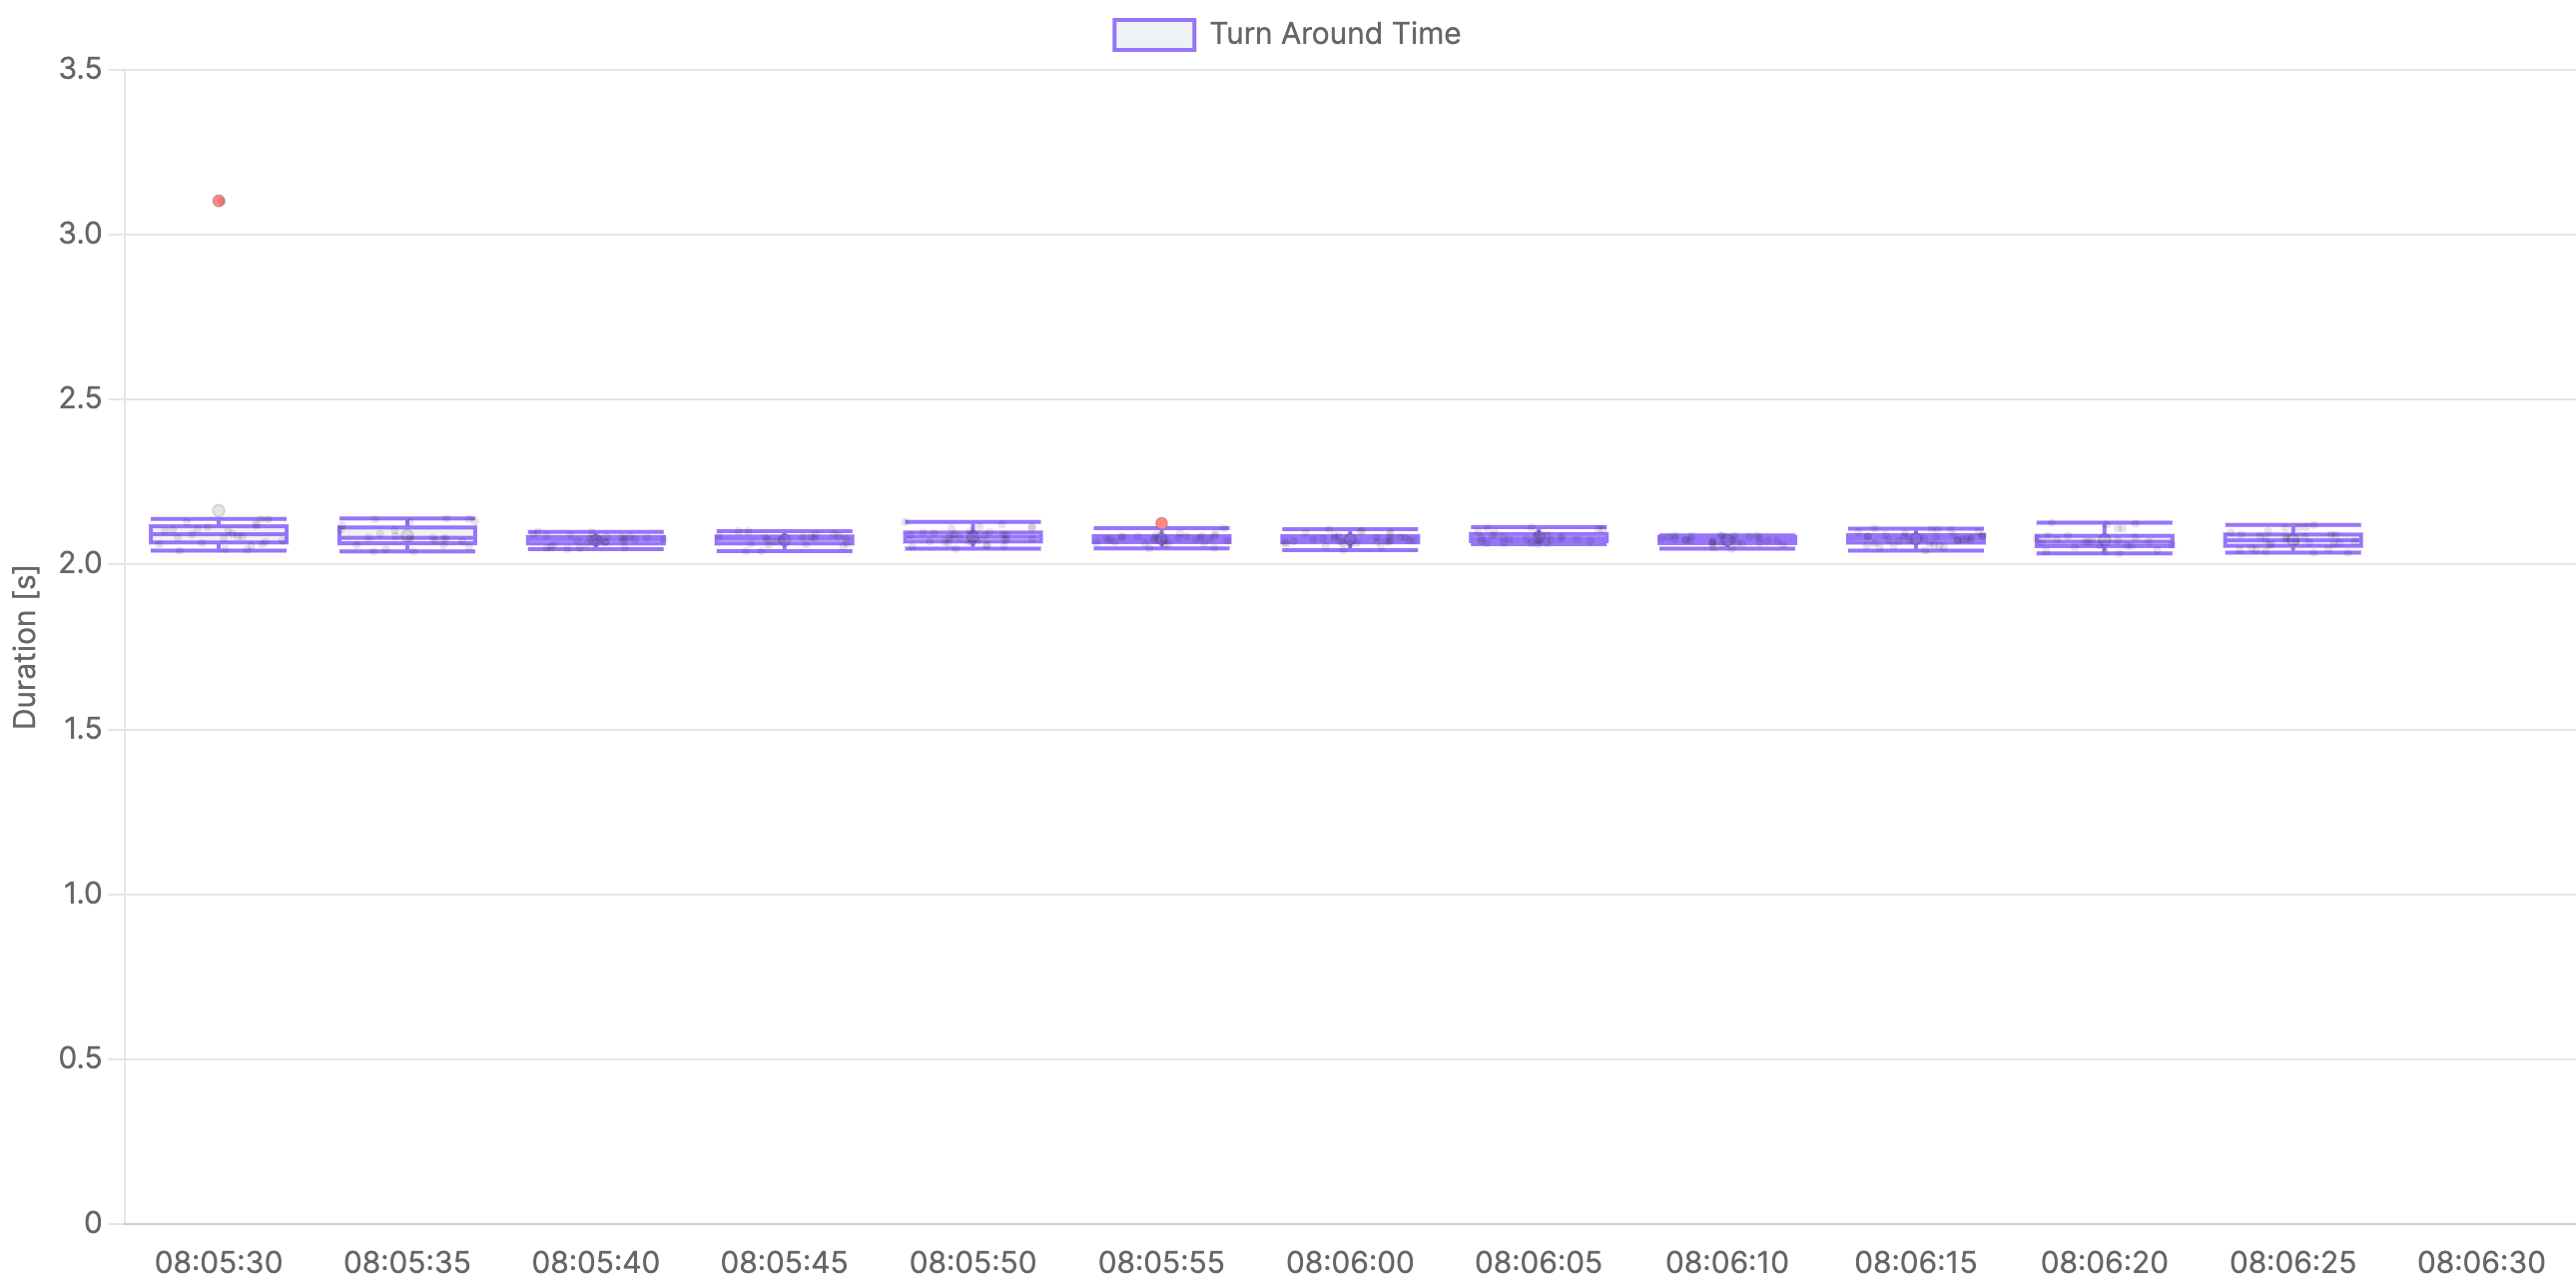
\includegraphics[width=0.89\textwidth]{images/Judge0 FER TAT for 5 5s.png}
	\caption{
		Vrijeme obrade zahtjeva FER-ove instance sustava Judge0 za $N=5$ i $M=60$ s asinkronom interakcijom.
	}
	\label{fig:judge0-fer-1}
\end{figure}

\begin{figure}[htb]
	\centering
	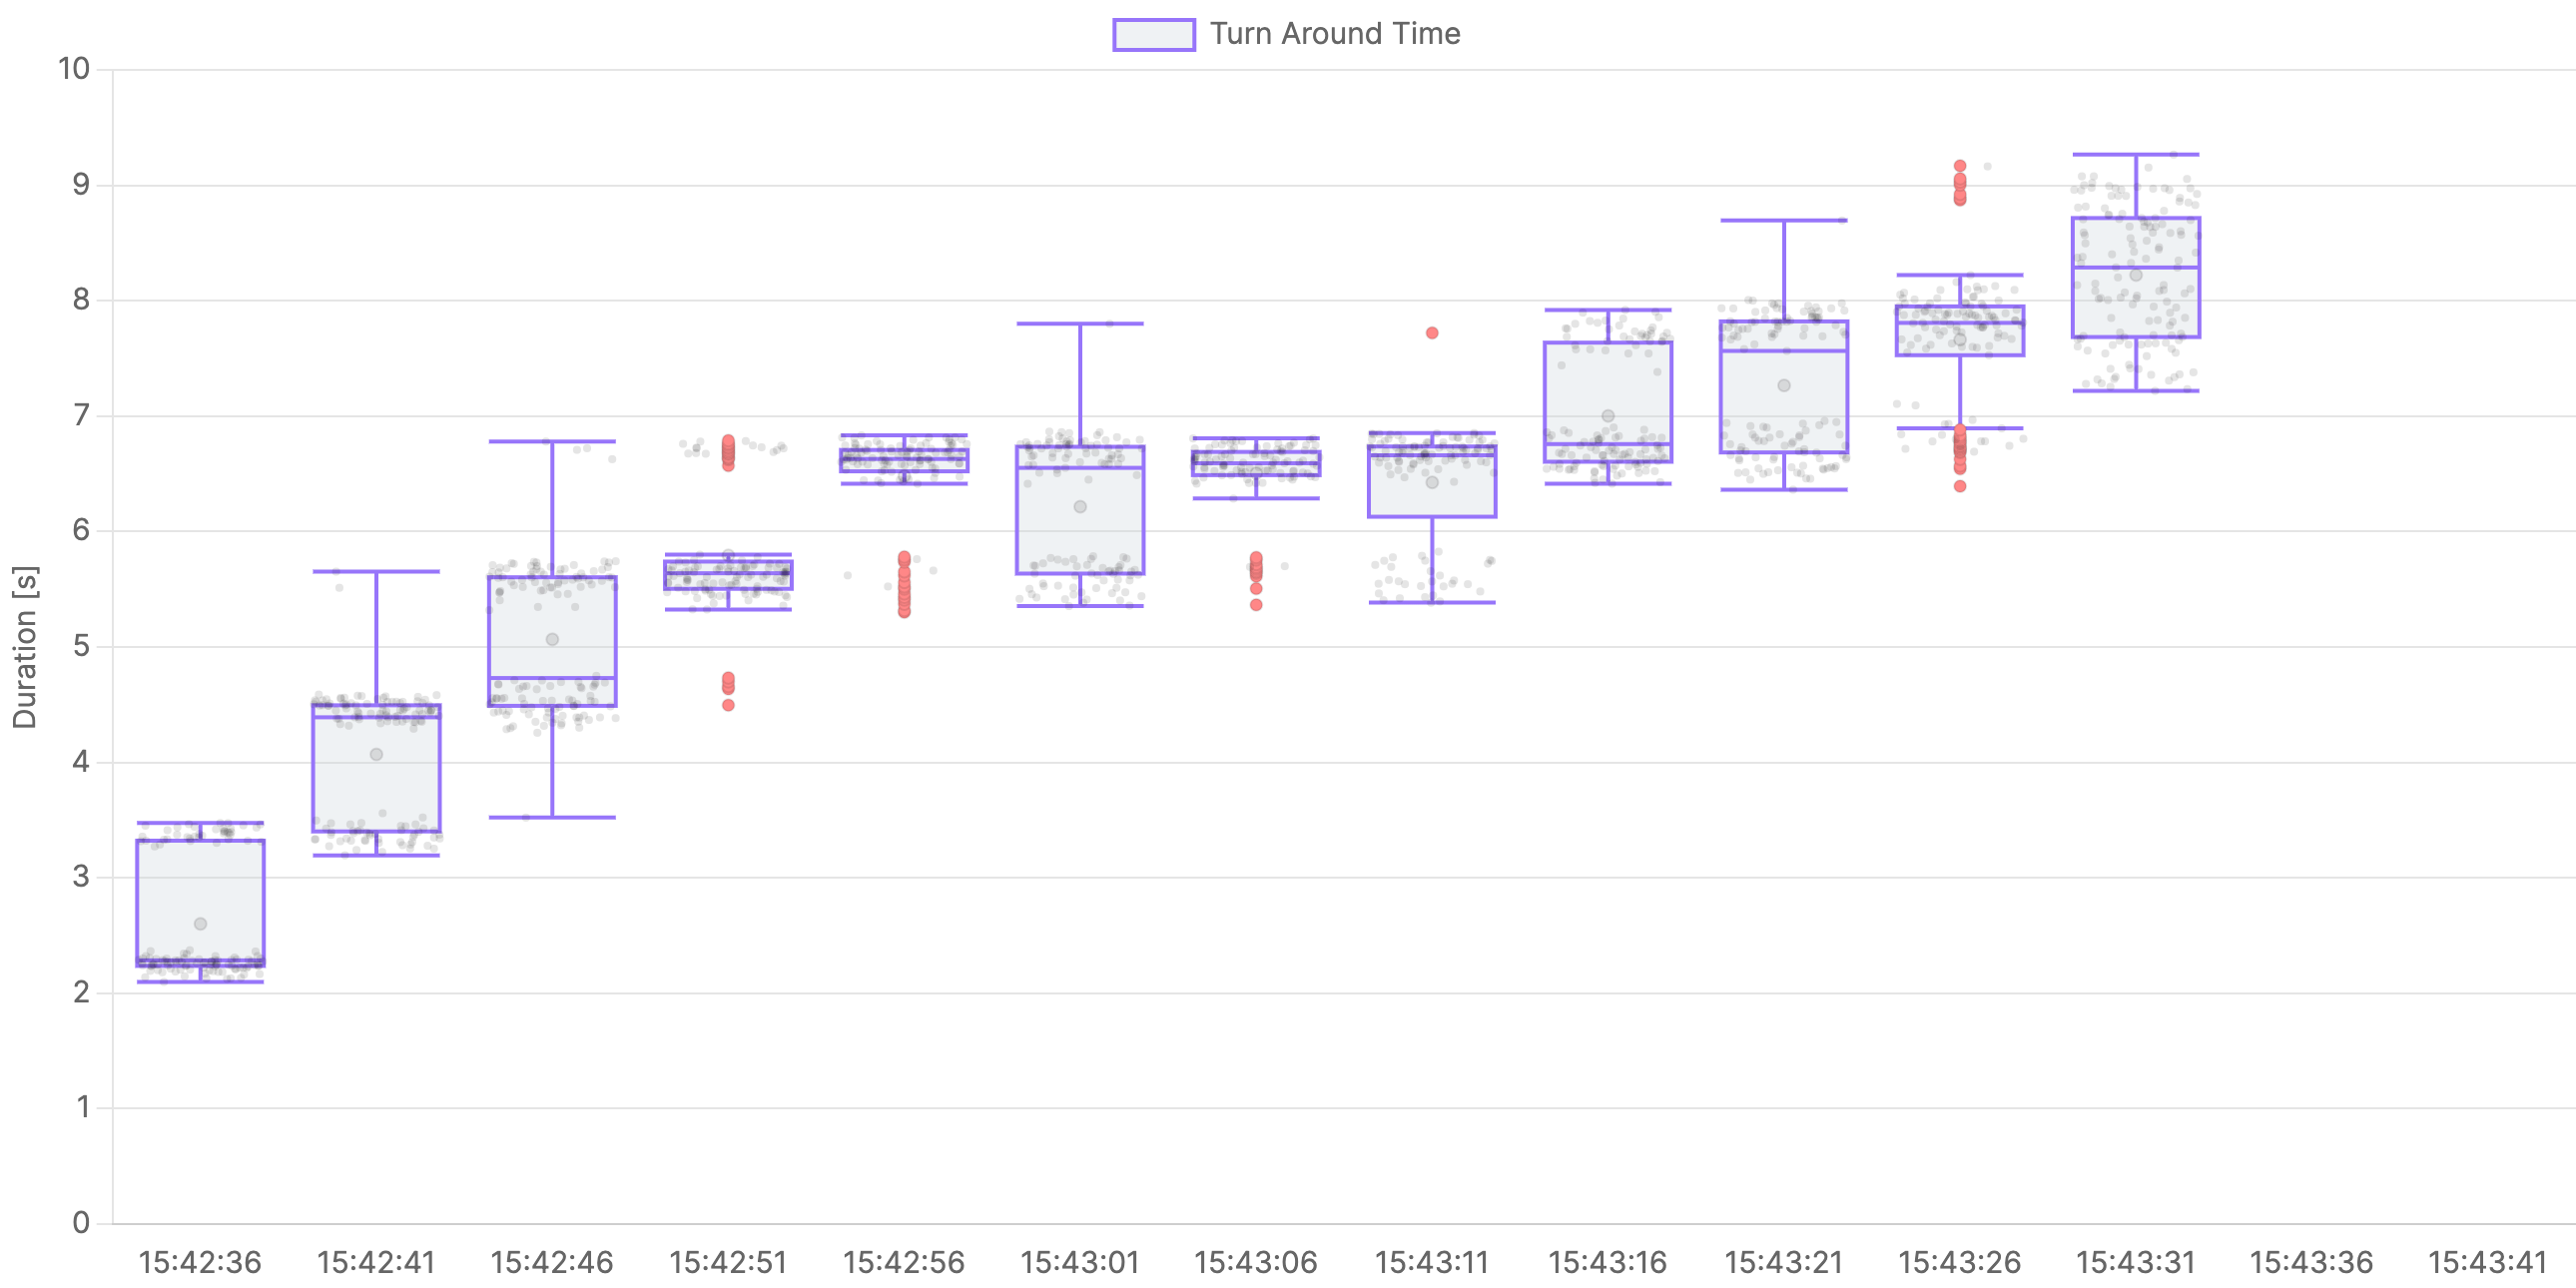
\includegraphics[width=0.89\textwidth]{images/Judge0 FER TAT for 25 5s.png}
	\caption{
		Vrijeme obrade zahtjeva FER-ove instance sustava Judge0 za $N=25$ i $M=60$ s asinkronom interakcijom.
	}
	\label{fig:judge0-fer-2}
\end{figure}

Dodatni eksperimenti napravljeni nad ovom instancom pokazuju kako je za sustav Judge0 uistinu nepovoljno koristiti sinkronu interakciju jer pri opterećenju od $N=5$ sustav uspješno obradi svega 70.21\% zahtjeva, dok medijan vrijeme obrade zahtjeva linearno raste s vremenom trajanja eksperimenta (slika \ref{fig:judge0-fer-3}). Službena, javno dostupna, instanca sustava Judge0 \citep{Judge0CE} nema problema sa rukovanjem ovog intenziteta opterećenja u sinkronoj interakciji. Njezino medijan vrijeme obrade zahtjeva ponaša se kao na slici \ref{fig:judge0-fer-1}, odnosno, kao i FER-ova instanca za asinkronu interakciju.

\begin{figure}[htb]
	\centering
	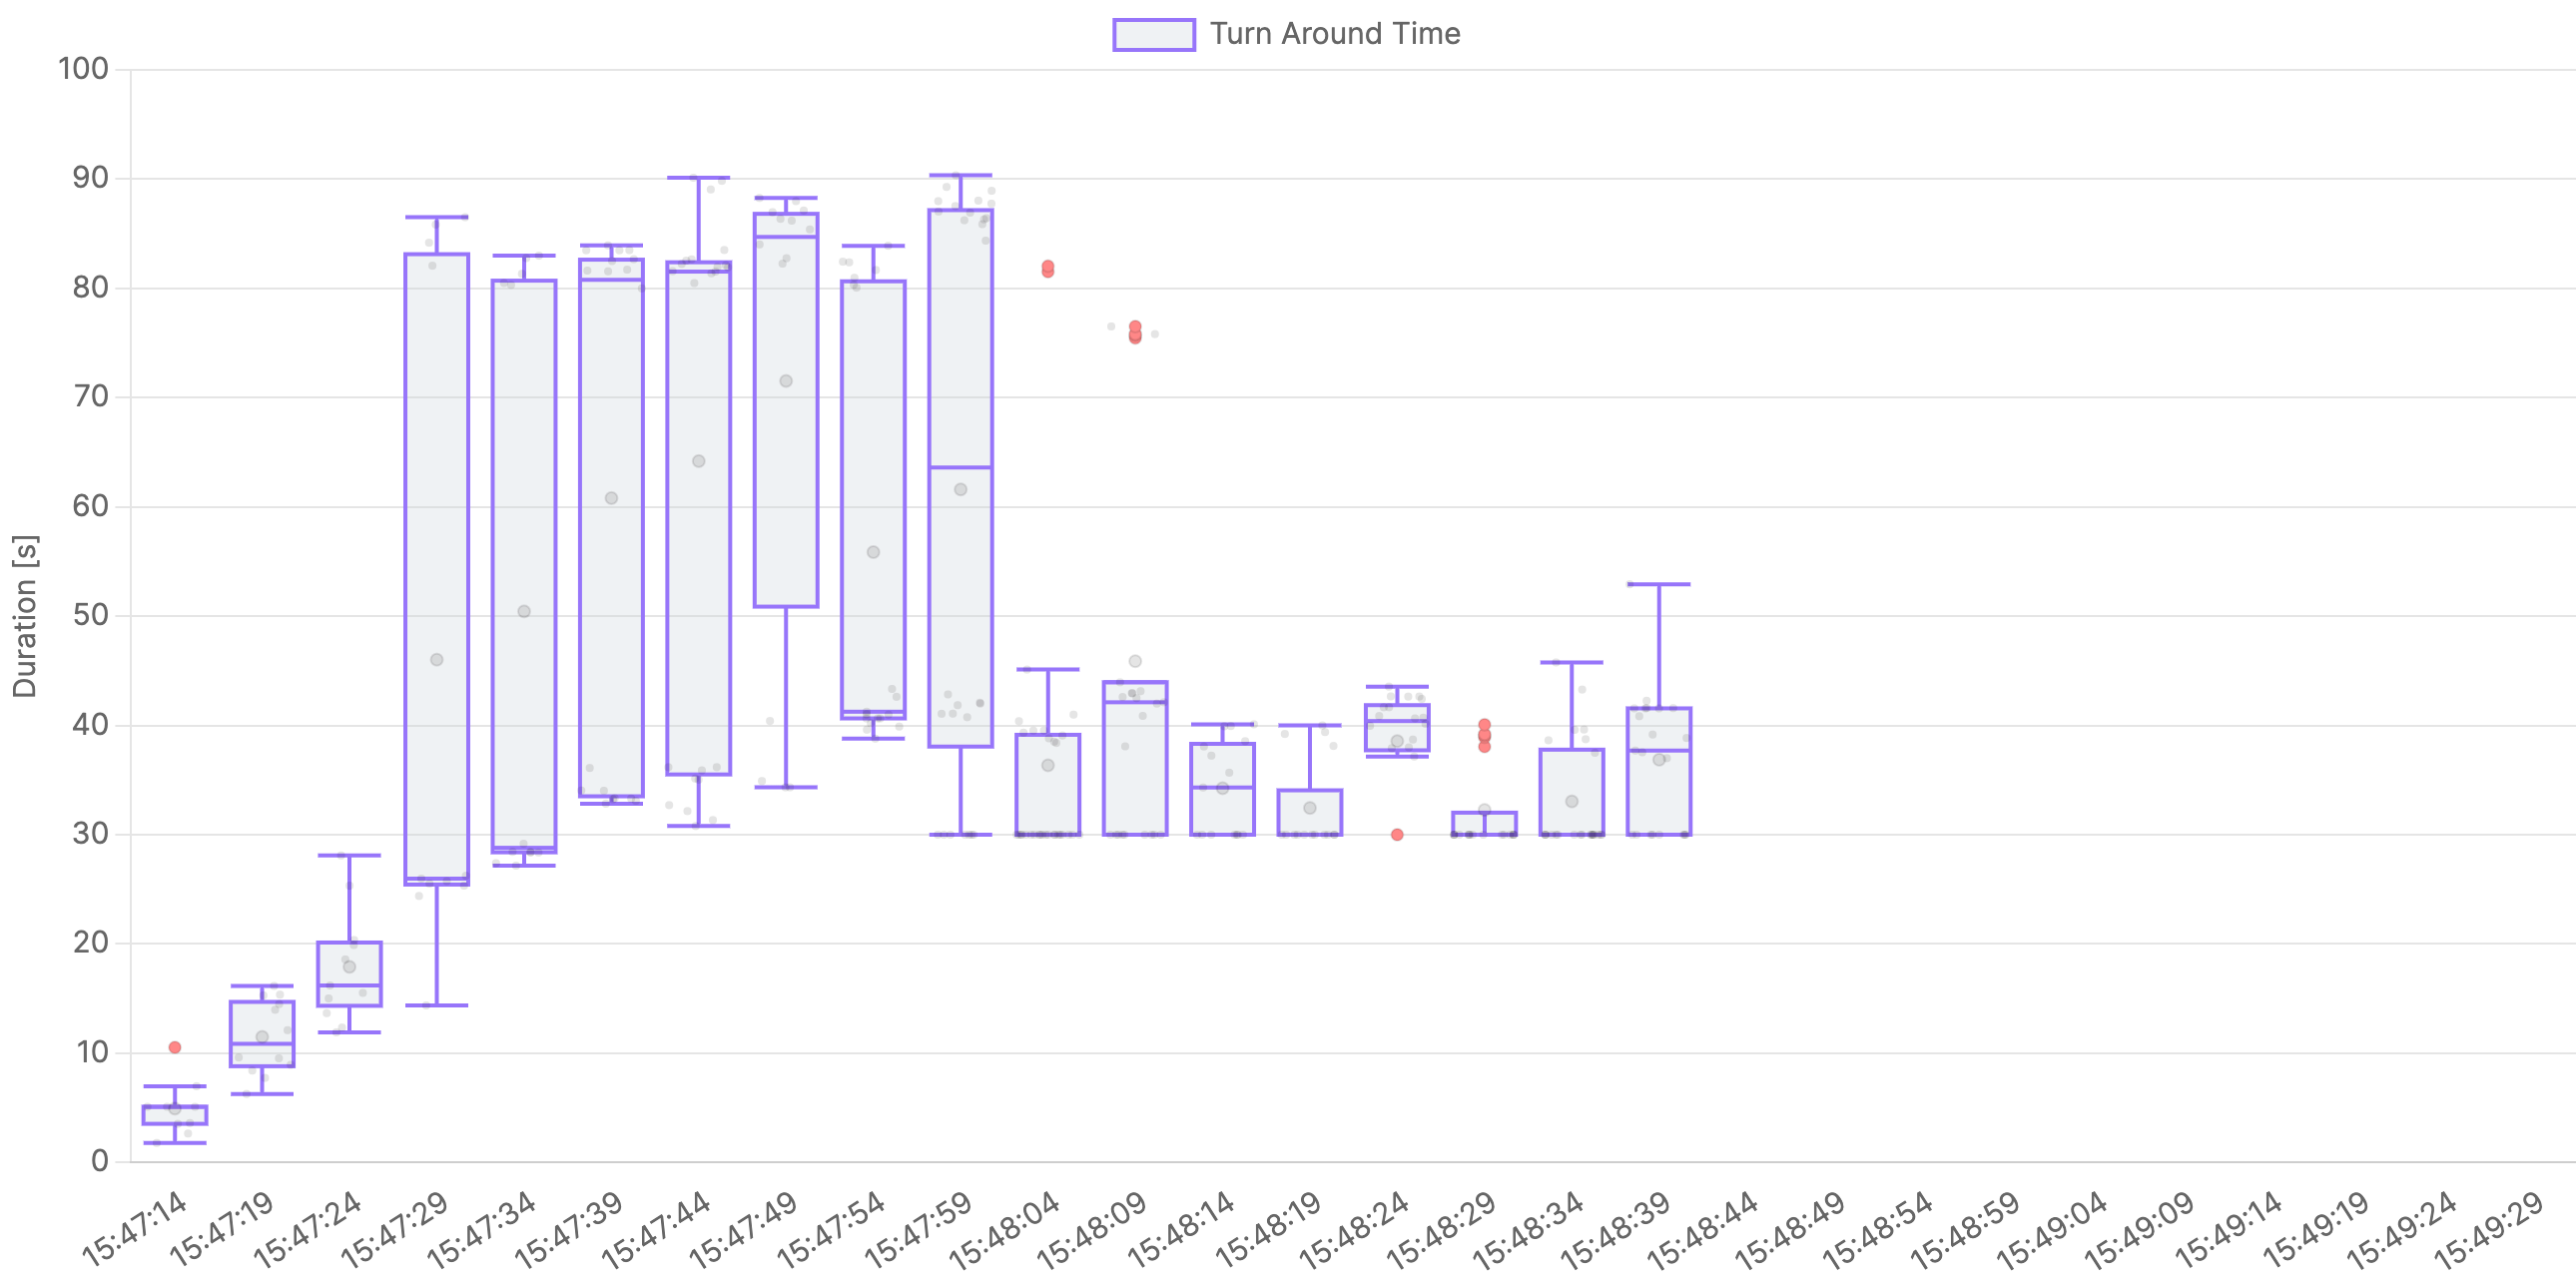
\includegraphics[width=\textwidth]{images/Judge0 FER TAT for sync 5 5s.png}
	\caption{
		Vrijeme obrade zahtjeva FER-ove instance sustava Judge0 za $N=5$ i $M=60$ sa sinkronom interakcijom.
	}
	\label{fig:judge0-fer-3}
\end{figure}

Eksperimenti pokazuju da FER-ova instanca sustava Judge0 podnosi srednje opterećenje od 20 zahtjeva u sekundi jednostavnog scenarija korištenja u \text{C++} implementaciji, dok za programski jezik Java ista instanca podnosi srednje opterećenje od 10 zahtjeva u sekundi, a za programski jezik Python čak 25 zahtjeva u sekundi.

Za razliku od jednostavnog scenarija korištenja, kod scenarija procesorskog opterećenja u \text{C++} implementaciji dolazi od rasta medijan vremena obrade već pri opterećenju od $N=5$ (slika \ref{fig:judge0-fer-4}), i isto ponašanje uočava se i u Java i Python implementaciji (slika \ref{fig:judge0-fer-5}).

\begin{figure}[htb]
	\centering
	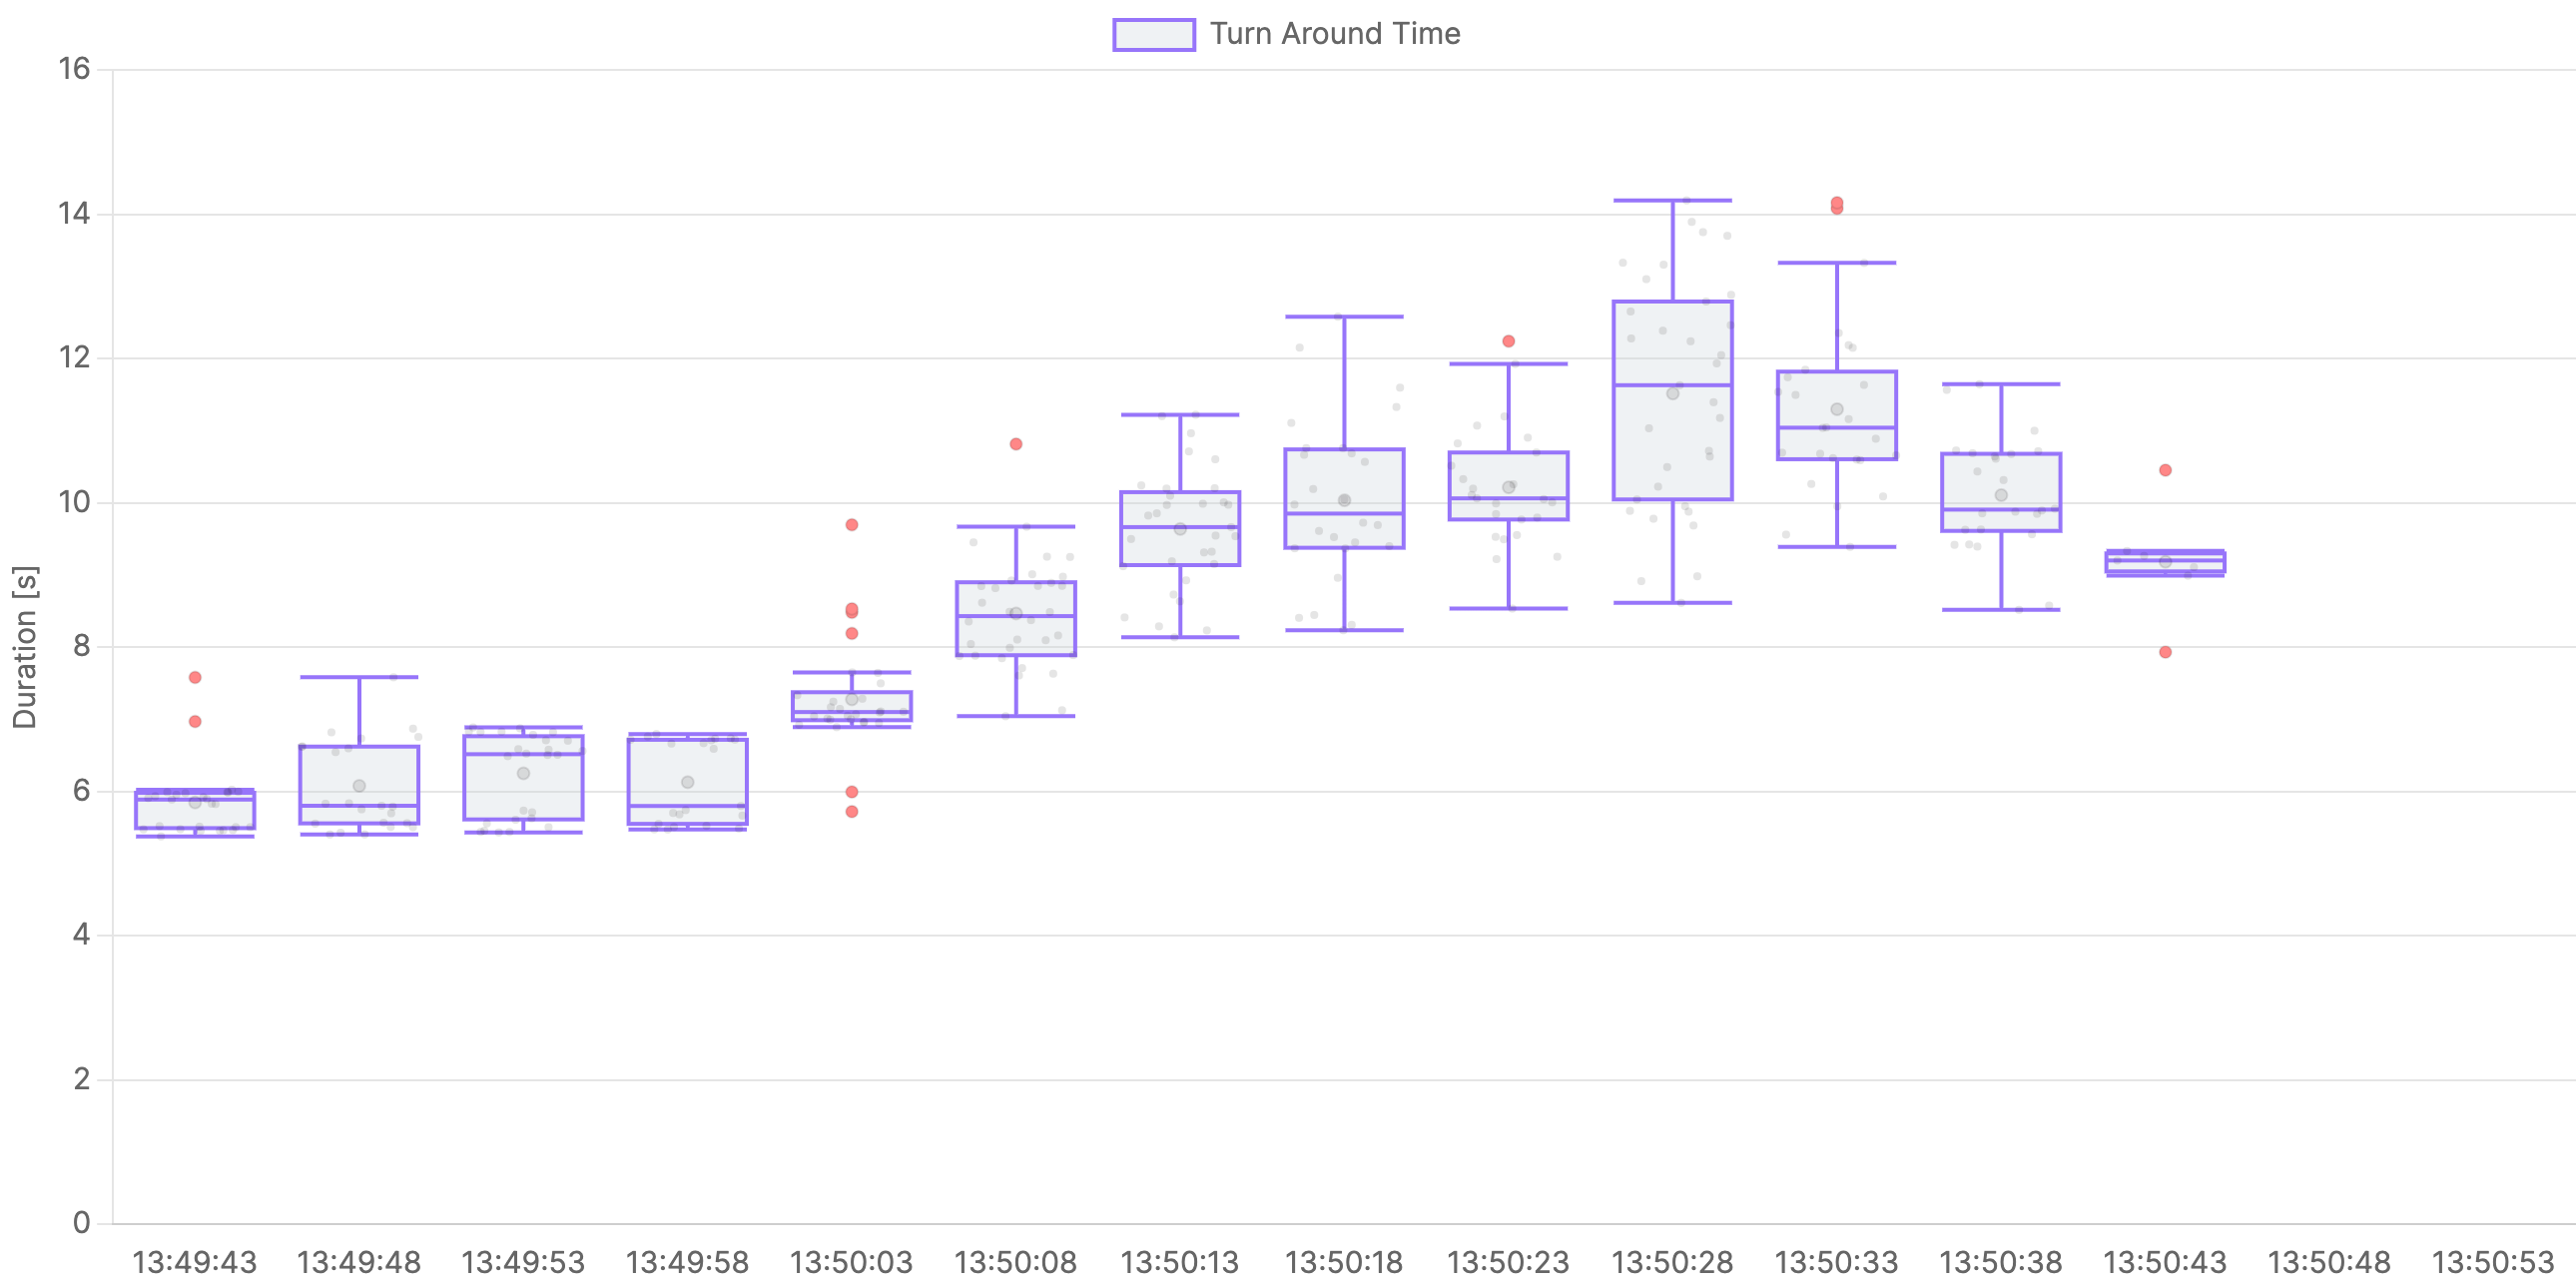
\includegraphics[width=\textwidth]{images/Judge0 FER TAT for CPU Intensive 5x60 5s.png}
	\caption{
		Vrijeme obrade zahtjeva FER-ove instance sustava Judge0 za $N=5$ i $M=60$ scenarija procesorskog opterećenja u \text{C++} implementaciji.
	}
	\label{fig:judge0-fer-4}
\end{figure}

\begin{figure}[htb]
	\centering
	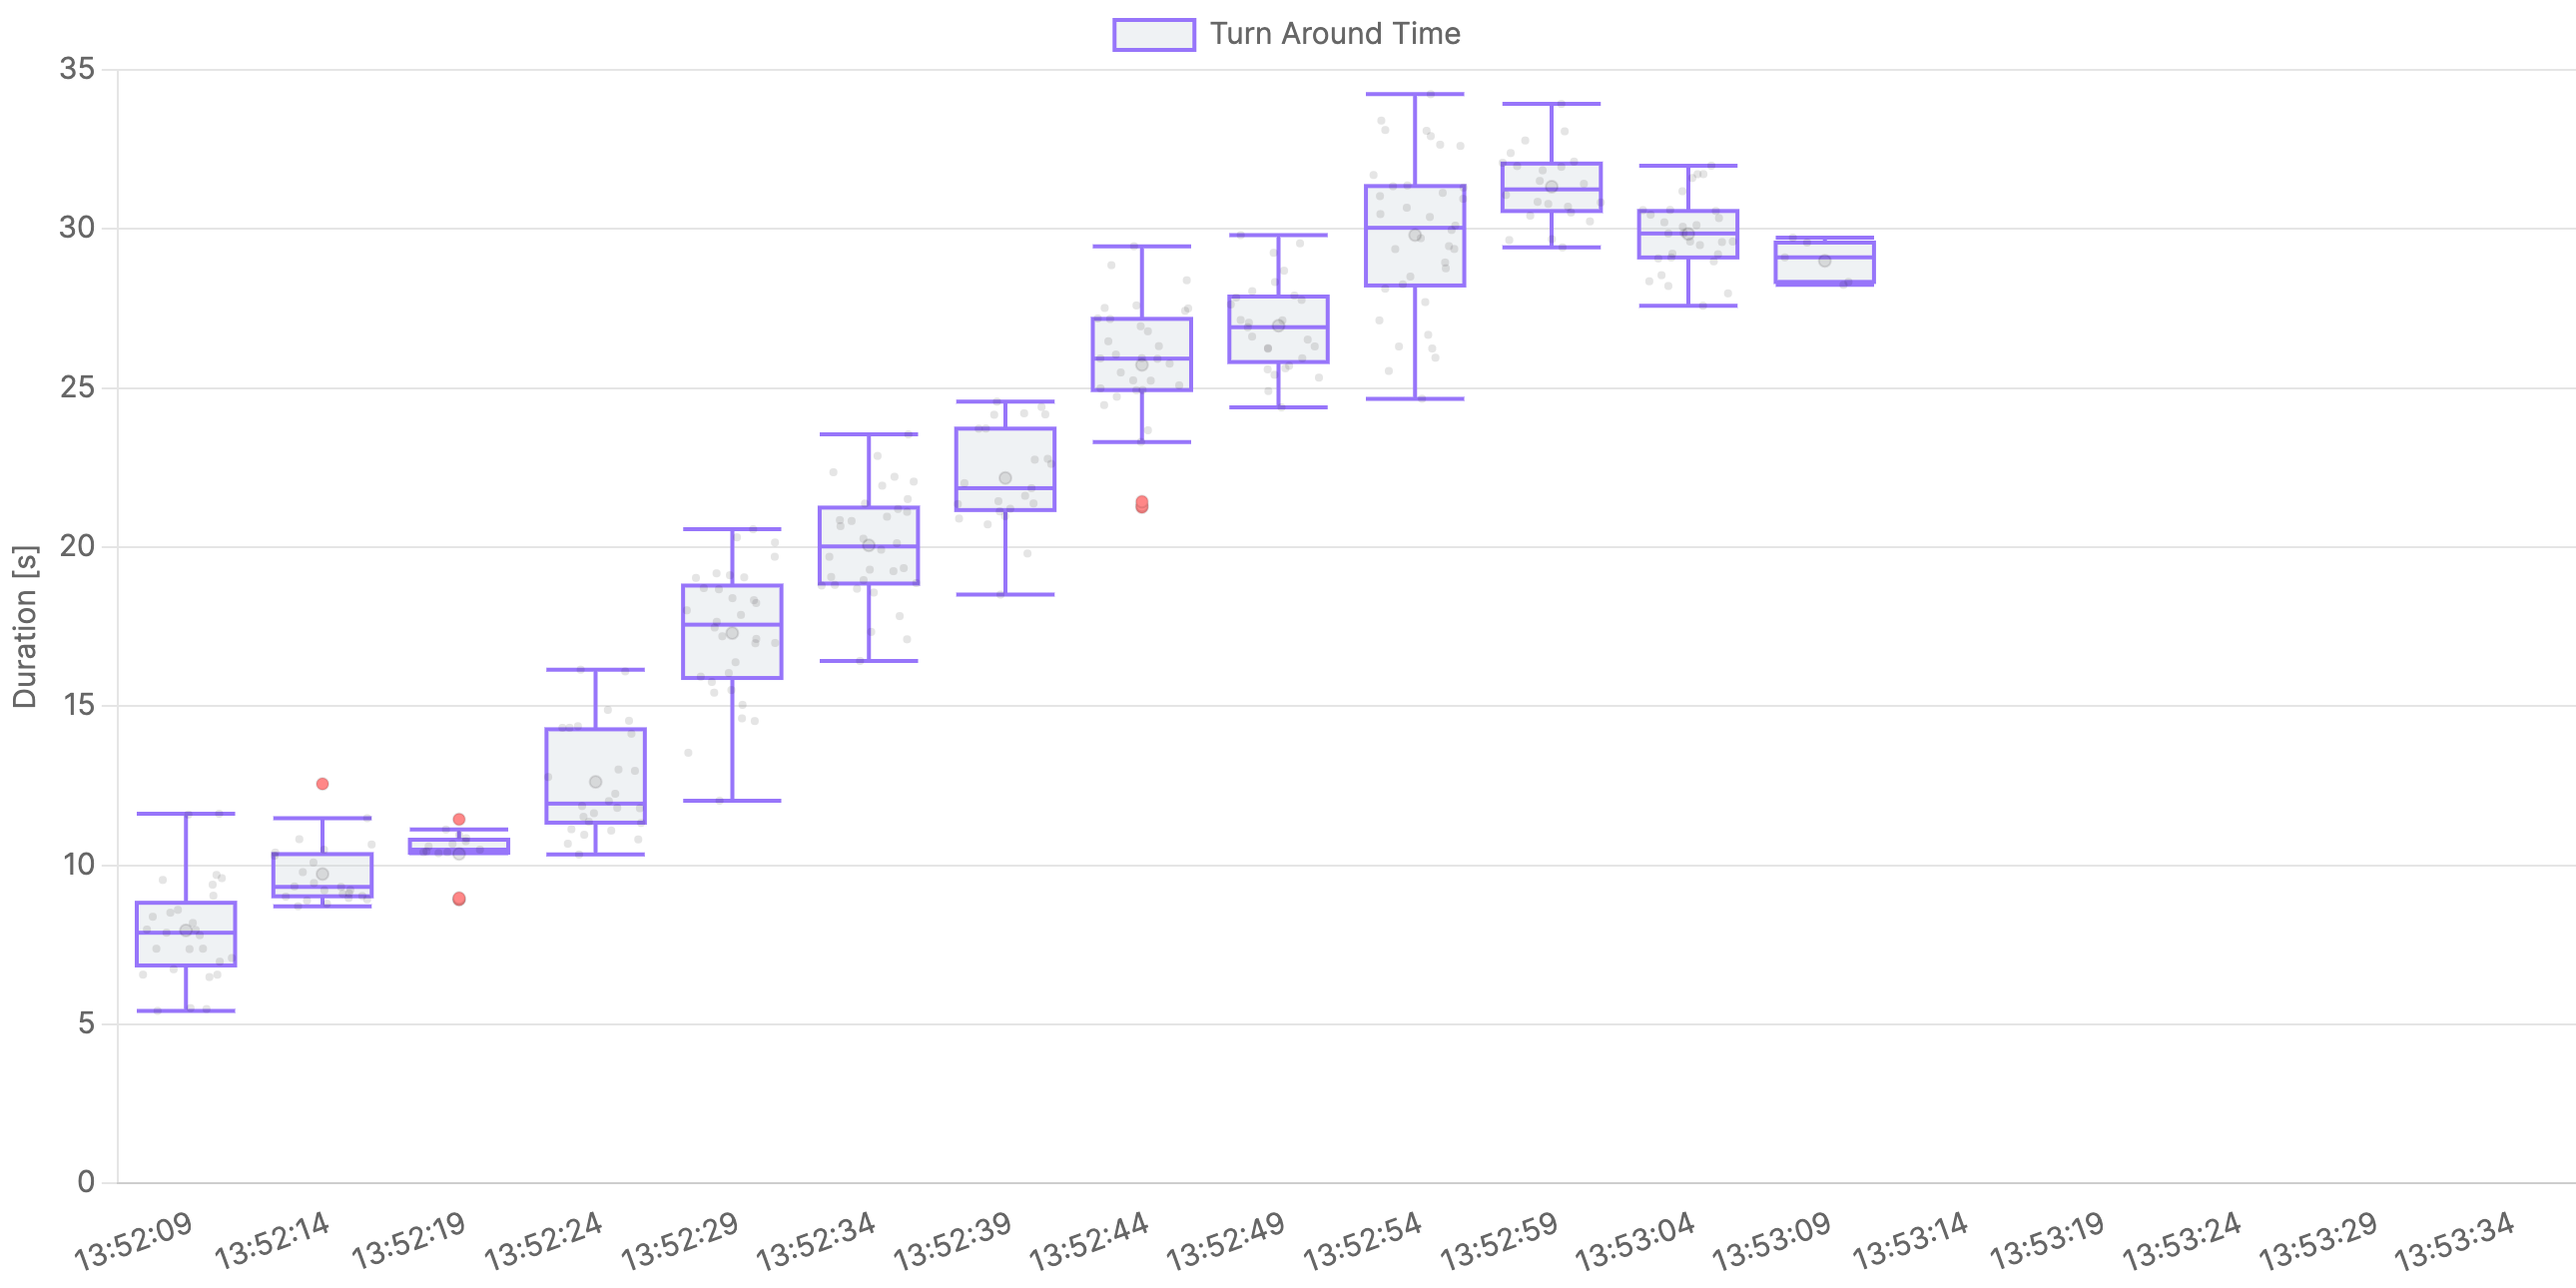
\includegraphics[width=\textwidth]{images/Judge0 FER TAT for CPU Intensive Java 5x60 5s.png}
	\caption{
		Vrijeme obrade zahtjeva FER-ove instance sustava Judge0 za $N=5$ i $M=60$ scenarija procesorskog opterećenja u Java implementaciji.
	}
	\label{fig:judge0-fer-5}
\end{figure}

\chapter{Budući razvoj}
\label{chap:future}
Za budući razvoj radnog okvira analize performansi i ocjene kvalitete i pouzdanosti preporučuje se razmatranje dodatnih metrika poput npr.\ trajanja slanja zahtjeva narudžbe. Za budući razvoj aplikacije Hélory preporuča se razvoj nove funkcionalnosti u grafičkom izvješću koja će omogućiti objedinjavanje i usporedbu rezultata više eksperimenata. Također, preporuča se implementacija automatskog traženja srednjeg opterećenja koje instanca podržava za odabrani scenarij korištenja i programski jezik. Za to je prije svega potrebno dobro definirati uvjet stabilne podrške nekog opterećenja. Dodatno, preporuča se detektiranje i implementacija dodatnih grafova koji se mogu dobiti koristeći sirove podatke prikupljene za vrijeme trajanja eksperimenta.

\chapter{Zaključak}
Sustav za udaljeno izvršavanje programskog kôda služe za sigurno i pouzdano izvršavanje korisničkog programskog kôda u sustavima za udaljeno ocjenjivanje koji se koriste u raznim slučajevima primjene među kojima su i \textit{web} aplikacije za e-učenje. U arhitekturi ekosustava sustava za udaljeno ocjenjivanje, sustavi za udaljeno izvršavanje programskog kôda promatraju se kao zasebne komponente u literaturi tek od \citep{9245310}. Budući da sustavi za udaljeno izvršavanje programskog kôda imaju ključni utjecaj na korisničko iskustvo, važno je da prilikom intenzivnog višekorisničkog opterećenja korisničko iskustvo ne pati zbog dugog vremena obrade zahtjeva za izvršavanje programskog kôda. Dosada u kontekstu sustava za udaljeno izvršavanje programskog kôda nisu postavljeni radni okviri za analizu njihovih performansi i ocjenu njihove kvalitete i pouzdanosti.

Ovaj rad predstavlja prvi radni okvir za analizu performansi i ocjenu kvalitete i pouzdanosti usluge koju nude sustavi za udaljeno izvršavanje programskog kôda. Ovaj rad također predstavlja i aplikaciju Hélory koja implementira predstavljeni radni okvir za analizu performansi i ocjenu kvalitete i pouzdanosti za tri sustava za udaljeno izvršavanje programskog kôda: Sphere Engine, Piston i Judge0. Razvijen u obliku komandno-linijske aplikacije, Hélory nudi jednostavno pokretanje višekorisničkog opterećenja na željenom sustavu, a nakon eksperimenta Hélory će generirati i pohraniti izvještaj o pokrenutom eksperimentu koji sadrži detaljne informacije o svakom pojedinom zahtjevu za izvršavanje i grafički prikaz metrika od interesa.

Koristeći aplikaciju Hélory eksperimentalno je dokazano da se pri korištenju sustava Judge0 preporuča koristiti asinkronu interakciju sa sustavom. Također provedeni eksperimenti nad instancom sustava Judge0 koja se koristi na Fakultetu elektrotehnike i računarstva Sveučilišta u Zagrebu pokazuju da instanca podnosi srednje opterećenje od 10 zahtjeva u sekundi jednostavnog scenarija korištenja u \text{C++} implementaciji, dok za programski jezik Java ista instanca podnosi srednje opterećenje od 5 zahtjeva u sekundi, a za programski jezik Python čak 20 zahtjeva u sekundi.

\bibliography{literatura}
\bibliographystyle{fer}

\begin{sazetak}
Sustavi za udaljeno izvršavanje programskog kôda imaju ključni utjecaj na korisničko iskustvo, i važno je da prilikom intenzivnog višekorisničkog opterećenja korisničko iskustvo ne pati zbog dugog vremena obrade zahtjeva za izvršavanje programskog kôda. Dosada u kontekstu sustava za udaljeno izvršavanje programskog kôda nisu postavljeni radni okviri za analizu njihovih performansi i ocjenu njihove kvalitete i pouzdanosti. Ovaj rad predstavlja prvi radni okvir za analizu performansi i ocjenu kvalitete i pouzdanosti usluge koju nude sustavi za udaljeno izvršavanje programskog kôda. Ovaj rad također predstavlja i aplikaciju Hélory koja implementira predstavljeni radni okvir za analizu performansi i ocjenu kvalitete i pouzdanosti za tri sustava za udaljeno izvršavanje programskog kôda: Sphere Engine, Piston i Judge0. Nakon pregleda osnovnih funkcionalnosti i sučelja aplikacije Hélory dan je primjer korištenja u analizi performansi sustava Piston i Judge0, ali i analiza performansi instance sustava Judge0 koja se aktivno koristi na Fakultetu elektrotehnike i računarstva Sveučilišta u Zagrebu. Konačno, na kraju se donose smjernice za budući razvoj radnog okvira i aplikacije.

\kljucnerijeci{analiza performansi, sustav za udaljeno izvršavanje programskog kôda, sustav za udaljeno ocjenjivanje, izvršavanje nepouzdanog programskog kôda, sphere engine, piston, judge0}
\end{sazetak}

\pagebreak

\engtitle{Performance analysis of online code execution systems}
\begin{abstract}
Online code execution systems have a crucial impact on the user experience, and it is essential that during intense multi-user workloads, the user experience does not suffer due to the long processing time of code execution requests. So far, in the context of online code execution systems, no framework has been made to analyze their performance and assess their quality and reliability. This paper presents the first framework for analyzing the performance and evaluating the quality and reliability of the service offered by online code execution systems. This paper also presents the Hélory application that implements the presented framework for performance analysis and quality and reliability assessment for three systems for online code execution: Sphere Engine, Piston, and Judge0. After reviewing the basic functionalities and interface of the Hélory application, an example of use in the performance analysis of the Piston and Judge0 systems is given, as well as the performance analysis of the Judge0 system instance actively used at the Faculty of Electrical Engineering and Computing, University of Zagreb. Finally, guidelines for the future development of the framework and application are given.

\keywords{performance analysis, online code execution system, online judge
system, untrusted code execution, sphere engine, piston, judge0}
\end{abstract}

\end{document}
